%! Mode:: "TeX:UTF-8"
%! TEX program = xelatex
\PassOptionsToPackage{quiet}{xeCJK}
\documentclass[withoutpreface,bwprint]{cumcmthesis}
\usepackage{etoolbox}
\BeforeBeginEnvironment{tabular}{\zihao{-5}}
\usepackage[numbers,sort&compress]{natbib}  % 文献管理宏包
\usepackage[framemethod=TikZ]{mdframed}  % 框架宏包
\usepackage{url}  % 网页链接宏包
\usepackage{subcaption}  % 子图宏包
\usepackage{makecell}
\usepackage{graphicx}
% \usepackage{enumerate}
\newcommand{\hei}{\CJKfamily{hei}}
% \usepackage{booktabs}
\newcolumntype{C}{>{\centering\arraybackslash}X}
\newcolumntype{R}{>{\raggedleft\arraybackslash}X}
\newcolumntype{L}{>{\raggedright\arraybackslash}X}

\title{基于高斯过程回归对超市收入的预测与优化}  % 论文标题
\tihao{}  % 题号
\baominghao{}  % 报名号
\schoolname{}  % 学校
\membera{}  % 队员a
\memberb{}  % 队员b
\memberc{}  % 队员c
\supervisor{}  % 指导老师
\yearinput{}
\monthinput{}
\dayinput{}

%%%%%%%%%%%%%%%%%%%%%%%%%%%%%%%%%%%%%%%%%%%%%%%%%%%%%%%%%%%%%
%% 正文
\begin{document}

\maketitle
\begin{abstract}%摘要
在零售行业数字化转型与消费者需求动态化的双重驱动下,
连锁超市的经营策略优化与收入预测正成为提升核心竞争力的关键课题。本文以国外某连锁超市三大店业务为研究对象,
基于2025年1月至4月的1000条交易数据,
从数据特征解析、预测建模与策略优化三维度出发,
构建融合Apriori关联规则挖掘、时间序列分析与多目标决策的综合模型体系,
实现了消费规律量化识别、毛收入动态预测及库存促销策略优化的全流程管理,为超市精细化运营与科学决策提供了数据驱动的解决方案。

\textbf{对于问题一,}
通过建立\textbf{TOPSIS模型},对会员与非会员对超时收入贡献度进行比较,
利用相关得分进行综合量化。在挖掘高频购买组合时,通过\textbf{Apriori算法},
提炼出置信度最高的组合。
综合分析各个指标可以得到,C店所在店的消费水平相对较高,并且三店消费时段集中在\textbf{10-11点,
13-15点,18-19点},而且\textbf{A 店使用电子钱包相对较多,而 B 店使用信用卡相对
较多,而 C 店相对使用现金较多}。
在TOPSIS模型量化下,会员群体对商店的贡献度比非会员高出5个百分点。
而高频购买组合是\textbf{运动旅游 + 信用卡 + 会员}。在大部分情况下,商品存在周末、节假日销量激增的现象。
\par

\textbf{对于问题二,}
先通过\textbf{KS正态检验}对所有数据检验,得到数据并不存在正态性分布,
由此在分析指标间关系时,通过斯皮尔曼相关性分析可知,
毛收入和商品单价、购买数量有着很强的正向相关性;毛利率和店、产品类别、购买数量有着很强的正向相关性。
在建立预测模型时,通过对比不同模型之间均方误差等参数的差异,最终选择\textbf{高斯过程回归机器学习模型}。
最终结果显示,最终选\textbf{GPR 模型预测} ,其误差低、适应性强,能为超市运营提供决策支撑。
\par

\textbf{对于问题三,}
本部分针对超市运营优化问题,基于销量对比分析、店铺评分评估及消费特征挖掘,提出两类战略建议。分析表明,食物类与运动旅行类商品需求突出,C 店经营表现显著优于 B 店(TOPSIS 模型评分验证),且消费者会员身份与其购买力呈现强相关性,为策略制定提供数据支撑。
在具体策略上,建议重点提升高需求品类库存并优化 C 店管理,结合需求波动动态调整安全库存,通过品类结构优化与精细化工具强化供给;同时设计分层会员权益,以组合消费激励形成正向循环。从战略布局看,鉴于 B 店区域生态恶化与 C 店所在城市的消费潜力,建议关闭 B 店释放资源,并在该城市科学拓店,复制成熟模式实现协同优化。
\par


% \textbf{对于问题四,}
% \par

\keywords{Topsis法\quad  傅立叶变换\quad  高斯过程回归\quad  Apriori算法 \quad 经营优化}
\end{abstract}
%%%%%%%%%%%%%%%%%%%%%%%%%%%%%%%%%%%%%%%%%%%%%%%%%%%%%%%%%%%%% 

% \tableofcontents  % 目录
% \newpage

%%%%%%%%%%%%%%%%%%%%%%%%%%%%%%%%%%%%%%%%%%%%%%%%%%%%%%%%%%%%%  
\section{问题重述}
\subsection{问题背景}
在全球零售行业数字化转型的进程中,
连锁超市作为现代流通体系的关键节点,
其运营模式正经历从经验驱动向数据驱动的深刻变革。
随着零售交易数据采集技术的精细化发展,
企业已积累海量包含商品属性、消费者行为轨迹、支付模式等多维信息的交易数据,
如何从这些数据中提炼商业洞察并构建科学决策体系,成为提升零售企业核心竞争力的战略课题。  
\par 某国外连锁超市在三大核心店构建商业网络,依托信息化管理系统对每笔交易进行全维度数据记录,
累计形成具有深度分析价值的数据集。当前企业管理层面临双重运营挑战:一方面,采购计划制定仍依赖传统经验判断,
导致库存配置与区域消费需求的动态匹配度不足,造成供应链效率损耗;另一方面,营销策略的精准性缺乏量化支撑,
难以针对不同客群的消费特征实现价值转化优化。这种数据资源与决策需求的结构性脱节,使得建立基于数据挖掘的收入预测体系成为企业突破经营瓶颈的必然选择。  
\par 由此可见,构建数据驱动的库存调度与智能排程方案,已成为布料企业突破运营瓶颈、提升综合竞争力的战略关键。


%%%%%%%%%%%%%%%%%%%%%%%%%%%%%%%%%%%%%%%%%%%%%%%%%%%%%%%%%%%%% 

\subsection{问题要求}
通过建立数学模型,结合超市的各商品的数据统计,
建立起相关科学的收入预测模型,以达到最小化成本,最大化利润的目标。
\par

\textbf{问题1:}  
基于该连锁超市2025年1月7日至4月5日的1000条交易数据,
需构建系统化的数据特征解析体系。
首先,运用统计学方法,
精确计算各店在销售额、商品单价、商品偏好等核心指标上的统计分布,通过交叉分析与时间序列建模,深入识别不同店在早、中、晚消费高峰时段及付款方式选择上的显著差异;其次,采用对比分析法与聚类算法,
细致剖析超市会员群体的消费特征,从消费频次、客单价、购买品类等维度量化会员与非会员群体的差异,并科学测算会员群体对超市总收入的贡献度;
再者,利用Apriori等关联规则算法,挖掘商品类别、付款方式、会员属性等多维度组合下的高频购买模式;最后,通过周期图分析与季节性分解,系统性探究六类商品销售数据的周期性特征,
识别周末、节假日等特殊时段的销量波动规律,为后续经营决策筑牢数据根基。
\par

\textbf{问题2:}  
针对超市毛收入与毛利率的预测需求,需搭建完整的数据分析与建模框架。
第一步,运用描述性统计、方差分析等方法,系统探究毛收入与毛利率在不同店、消费者类别、产品类别、付款方式等维度的分布规律,
借助热力图、箱线图等可视化手段直观呈现分析结果,并通过相关性检验与显著性分析,
精准识别对毛收入与毛利率具有显著影响的关键变量;
第二步,综合运用时间序列模型、回归分析及机器学习算法构建预测模型,对2025年4月6日至15日超市日均毛收入与毛利率进行预测。通过均方误差(MSE)、平均绝对误差(MAE)等指标对比不同模型的预测精度,
结合数据特征与业务场景,合理阐释模型选择依据;
同时,结合该国节假日日历,评估特殊节假日对销售数据的影响,
在模型中科学引入虚拟变量或季节性调整因子,确保预测结果的准确性与可靠性。
\par


\textbf{问题3:} 
基于上述数据分析与模型结果,从战略决策与运营优化层面,
为超市管理层提供具有实操性的量化经营策略优化建议。
其一,通过需求预测与边际收益分析,精准确定需优先提升库存水平或加大促销力度的商品类别、店区域及客户群体;
其二,建立客户满意度评分与经营指标的关联模型,提出针对性的服务流程优化与产品改进方案;
其三,运用组合优化算法,设计提升毛利率的商品组合策略,并通过模拟分析验证策略有效性;
其四,结合各店销售数据特征与需求预测结果,制定差异化的库存优化方案;
其五,构建会员扩容对收入影响的弹性模型,预测会员占比提升10\%时的收入增长幅度;
其六,建立多目标决策模型,综合考量收入损失、客户流失率、区域竞争态势等因素,
为超市关店决策提供科学的量化评估框架,助力企业实现资源的高效配置与竞争力的全面提升。

\par


% \textbf{问题4}  
% \par

% \par


%%%%%%%%%%%%%%%%%%%%%%%%%%%%%%%%%%%%%%%%%%%%%%%%%%%%%%%%%%%%% 

\section{问题分析}
\subsection{问题一分析}
对于问题一,需从多维度解析数据特征与挖掘规律。
首先,针对三大城市的销售数据,需计算销售额、商品单价、商品偏好等指标的统计分布,如通过分组计算各城市不同商品类别的销量占比、销售额均值及单价分位数,
同时分析早(10-11 点)、中(13-15 点)、晚(18-19 点)高峰时段的交易分布差异,以及 A 店电子钱包、B 店信用卡、C 店现金的支付方式选择偏好。
其次,分析会员消费特征时,利用 TOPSIS 模型量化会员与非会员的贡献度差异,发现会员贡献度较非会员高 5 个百分点,结合客单价、购买频次等指标深入对比两类群体的消费行为。
再者,运用 Apriori 算法挖掘高频购买组合,提炼出 “运动旅游 + 信用卡 + 会员” 这一置信度最高的组合,需验证其支持度与提升度以确认商业价值。
最后,分析六类商品的销售周期性,关注周末及节假日是否存在销量激增现象,例如通过时间序列分解识别周期性波动规律。
整个分析过程需结合数据预处理与可视化手段,为后续预测与策略优化提供数据支撑。

\subsection{问题二分析}	
在解决超市毛收入与毛利率预测问题时,需从数据特性分析与模型构建逻辑展开系统分析。
首先,通过KS正态性检验发现数据不服从正态分布,这决定了传统基于正态假设的统计方法适用性受限。
其次,采用非参数的斯皮尔曼相关性分析,探究指标间关系。再者,在构建预测模型时,对比时间序列、传统回归与机器学习模型的均方误差、平均绝对误差等指标,以选择合适模型。
此外,模型构建需考虑预测期内是否包含节假日,若存在则需引入相应变量调整预测结果,确保模型鲁棒性,
最终实现对未来十天日均毛收入与毛利率的精准预测,为超市相关策略提供量化支撑。

\subsection{问题三分析}
对于问题三,在解决超市库存优化与店铺布局问题时,需从经营数据特征与策略逻辑展开系统分析。首先,通过销售数据的趋势分解发现食物类与运动旅行类商品存在显著季节性波动,这决定了传统固定库存策略的局限性。其次,采用TOPSIS综合评价法探究店铺运营效率,量化C店与B店的综合表现差异。再者,在制定库存与拓店策略时,对比ABC分类法、层次分析法与动态规划模型的资源配置效率,以确定最优方案。此外,策略设计需考虑区域消费特征,若C店所在城市存在消费升级趋势则需引入差异化品类布局,确保策略针对性。最终实现库存周转率提升与店铺网络优化的协同,为超市战略决策提供量化支撑。

% \subsection{问题四分析}
% 对于问题四,

%%%%%%%%%%%%%%%%%%%%%%%%%%%%%%%%%%%%%%%%%%%%%%%%%%%%%%%%%%%%% 

\section{模型假设}

为了构建更加精准的数学模型,本文根据实际情况以及任务所给要求做出以下合理的假设或条件约束:

\begin{itemize}[itemindent=2em]
\item 假设超市交易数据记录完整,无系统性缺失或录入错误,各类指标的统计口径一致,可直接用于模型分析。
\item 假设预测期内消费者的购买偏好、会员活跃度及支付习惯与历史数据表现一致,不出现突发性消费趋势转变。
\item 假设 C 店所在城市的消费升级趋势、B 店所在区域的商业生态在短期内无显著变化,拓店选址的竞争格局与成本结构保持稳定。
\item 假设库存优化策略中引入的安全库存模型、ABC 分类法等工具可有效执行,供应链响应速度满足动态补货需求,且商品损耗率控制在行业常规水平。
\item 假设分层会员权益、动态折扣等政策可被消费者清晰认知,且优惠成本与激励效果呈线性正相关,不存在因政策复杂导致的参与度低下问题。
\item 假设 TOPSIS 模型、高斯过程回归等方法的评价维度与预测逻辑符合超市实际经营场景,模型参数的优化结果具备商业解释性。
\end{itemize}

%%%%%%%%%%%%%%%%%%%%%%%%%%%%%%%%%%%%%%%%%%%%%%%%%%%%%%%%%%%%% 

\section{符号说明}
\begin{table}[H]
\centering
\begin{tabularx}{\textwidth}{CLC}
\toprule
符号    & 说明    & 单位 \\
\midrule
$\mu    $& 样本均值 & $\text{个}$ \\
$\sigma     $& 样本标准差 & $\text{无}$ \\
$D    $& 经验分布与理论正态分布的最大垂直距离 & $\text{无}$ \\
$\epsilon    $& 独立同分布的噪声 & $\text{无}$ \\
$\phi_i    $& 自回归系数 & $\text{无}$ \\

\bottomrule
\end{tabularx}
\label{tab:符号说明}
\end{table}


%%%%%%%%%%%%%%%%%%%%%%%%%%%%%%%%%%%%%%%%%%%%%%%%%%%%%%%%%%%%% 

\section{问题一的模型的建立和求解}
\subsection{TOPSIS模型的建立}
TOPSIS模型是一种常用的多属性决策性模型。其核心思路是基于归一化决策矩阵,
通过计算各个评价对象和最优方案、最劣方案的相对接近程度,从而评价对象排序。\upcite{behzadian2012state}
\par
\textbf{Step1} 正向化处理表格数据
\par
本题中,由于数据均为正向化数据,因此小组跳过了本步骤。

\par
\textbf{Step2} 标准化处理表格数据
\par
标准化处理表格数据最大目的是在于其能够消除不同指标的量纲带来的影响。
在本题中,有501个评价对象即会员总数,2个评价指标(即毛收入和毛利率),以此构建出标准化矩阵X如下:
\begin{equation}
\label{eq:公式1}
X_1=
\begin{bmatrix}
x_{11} & x_{12} & x_{13} \\
x_{21} & x_{22} & x_{23} \\
\vdots & \vdots & \vdots \\
x_{(501)1} & x_{(501)2} & x_{(501)3}
\end{bmatrix},
\end{equation}
然后,对标准化后的矩阵Z中的每一个元素进行如下操作:


\begin{equation}
\label{eq:公式1}
z_{ij}=\frac{x_{ij}}{\sqrt{\sum_{i=1}^nx_{ij}^2}},i=1,2,3\quad j=1,2,...,4000
\end{equation}

\textbf{Step3} 计算得分并归一化处理
\par
这些指标的标准化矩阵Z表示为:
\begin{equation}
\label{eq:公式1}
Z_1=
\begin{bmatrix}
z_{11} & z_{12} & z_{13} \\
z_{21} & z_{22} & z_{23} \\
\vdots & \vdots & \vdots \\
z_{(501)1} & z_{(501)2} & z_{(501)3}
\end{bmatrix},
\end{equation}
\par
定义最大值:
\begin{equation}
\label{eq:公式1}
Z^{+}=\binom{\max \left\{z_{11}, z_{21}, \ldots, z_{(501) 1}\right\}}{\max \left\{z_{12}, z_{22}, \ldots, z_{(501) 2}\right\}, \max \left\{z_{13}, z_{23}, \ldots, z_{(501)3}\right\}},
\end{equation}

\par
定义最小值:
\begin{equation}
\label{eq:公式1}
Z^{+}=\binom{\min \left\{z_{11}, z_{21}, \ldots, z_{(501) 1}\right\}}{\min \left\{z_{12}, z_{22}, \ldots, z_{(501) 2}\right\}, \max \left\{z_{13}, z_{23}, \ldots, z_{(501)3}\right\}},
\end{equation}

\par
计算距离:
\begin{itemize}
\item 	第i个评价对象与最大值的距离:
\par
\begin{equation}
\label{eq:公式1}
D_{i}^{+}=\sqrt{\sum_{j=1}^{m}\left(Z_{j}^{+}-Z_{i j}\right)^{2}},
\end{equation}

\item 	第i个评价对象与最小值的距离:
\begin{equation}
\label{eq:公式1}
D_{i}^{-}=\sqrt{\sum_{j=1}^{m}\left(Z_{j}^{-}-Z_{i j}\right)^{2}},
\end{equation}
\end{itemize}

\textbf{Step4} 计算得分
\begin{equation}
\label{eq:公式1}
S_i=\frac{D_i^-}{D_i^++D_i^-},
\end{equation}

\subsection{TOPSIS模型得分}
我们将毛利数据带入到上述TOPSIS模型中,可以得到以下得分:
\begin{figure}[H]
\centering
\subcaptionbox{非会员TOPSIS模型得分\label{fig:双图a}}
{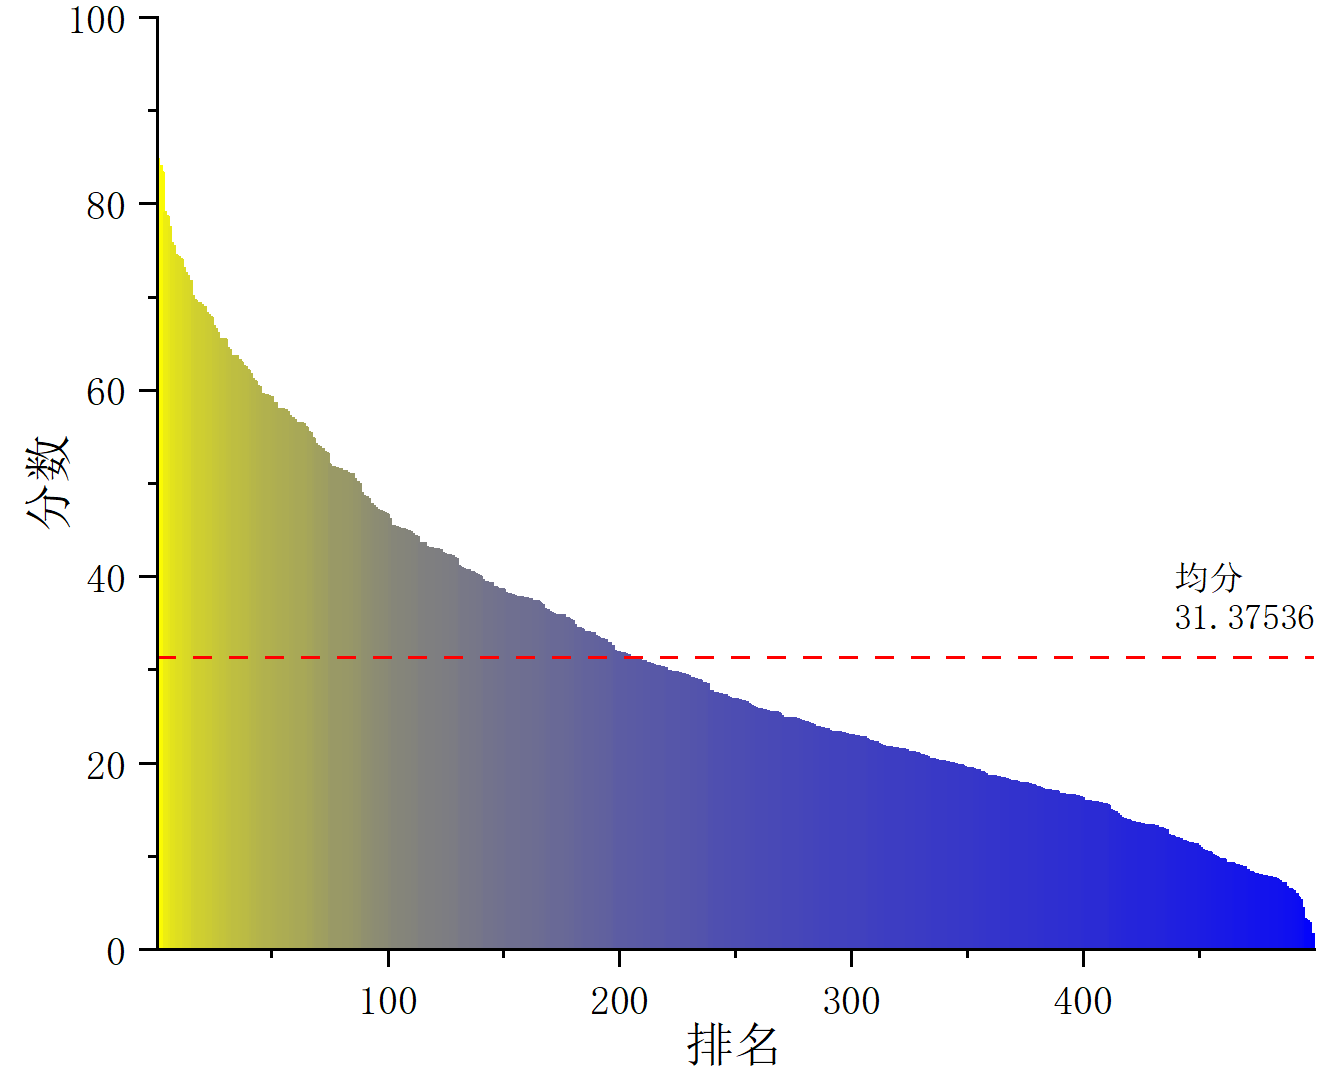
\includegraphics[width=.4\textwidth]{非会员TOPSIS模型得分.png}}
\subcaptionbox{会员TOPSIS模型得分\label{fig:双图b}}
{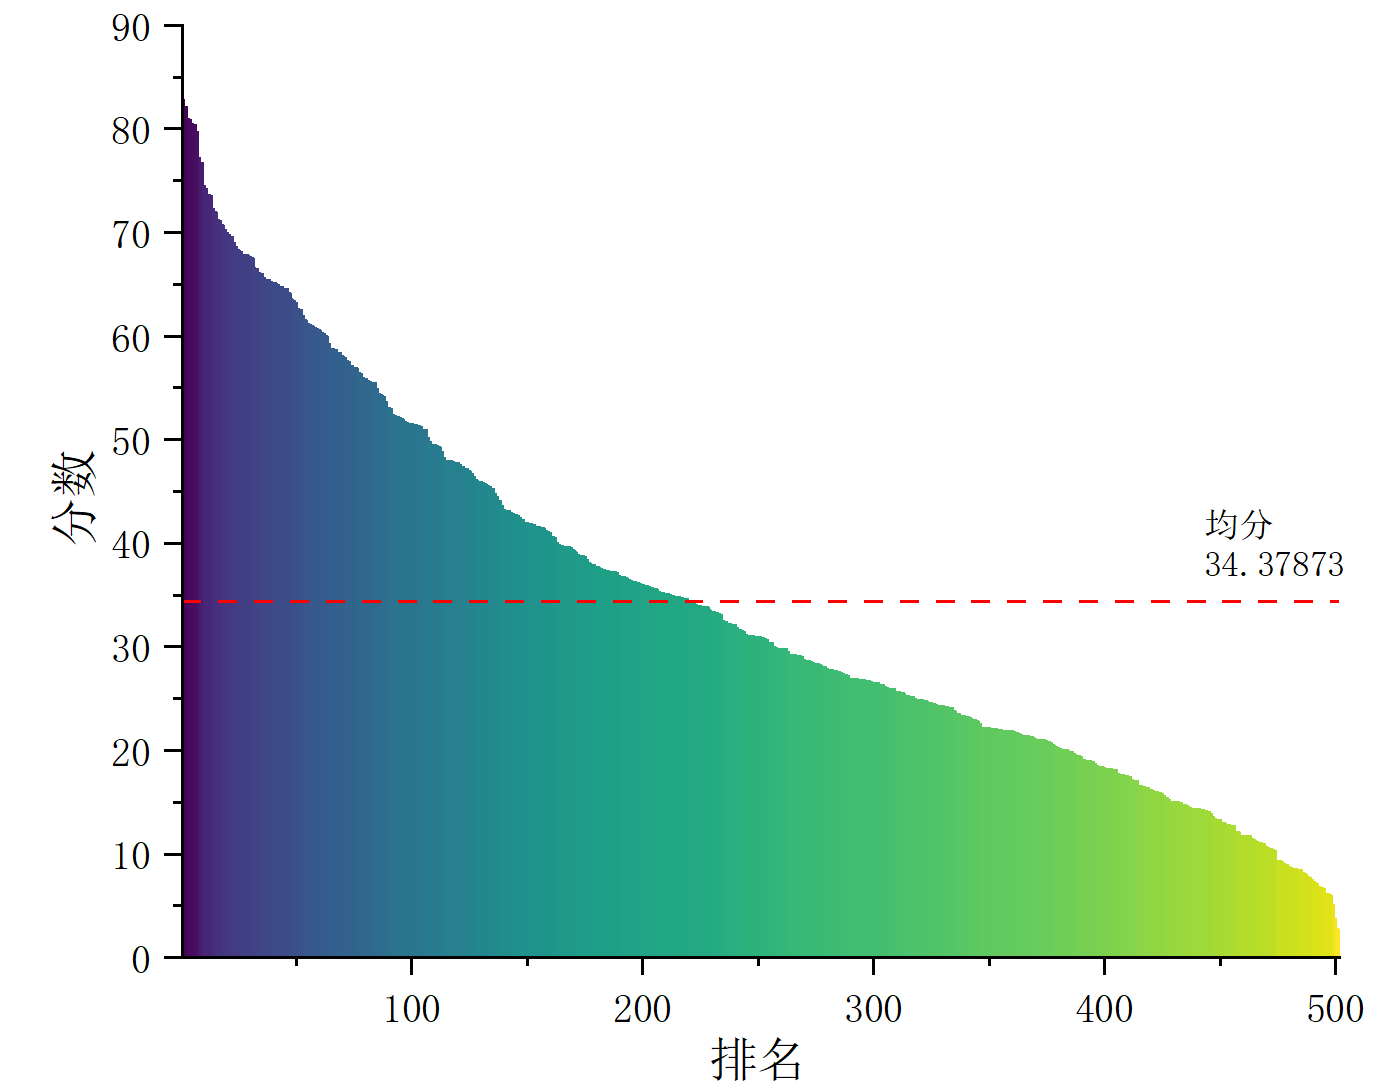
\includegraphics[width=.4\textwidth]{会员TOPSIS模型得分.png}}
\caption{TOPSIS模型得分}\label{fig:双图}
\end{figure} 
由上图对比可知,会员群体的平均贡献度为34.38,并且总体上要高于非会员的贡献度。

\subsection{关联算法规则算法的应用}

\subsubsection{定义支持度阈值}
\textbf{支持度:}支持度表示项集在所有交易中出现的频率,其公式为:
\begin{equation}
\label{eq:公式1}
\text{Support}(X) = \frac{\text{包含项集X的交易数}}{\text{总交易数}} \
\end{equation}
初始可设阈值为 0.05-0.1,通过 “支持度 - 频繁项集数量” 曲线调整,避免遗漏潜在模式或产生噪声。
\par
\textbf{最小支持度的确定:}先设定一个初始值(5\%),在观察频繁项集的数量和合理性后,逐步调整相关阈值,找到曲线的拐点作为合适阈值。
调整过程如下图:
\begin{figure}[H]
    \centering
    \subcaptionbox{Step1\label{fig:双图a}}
    {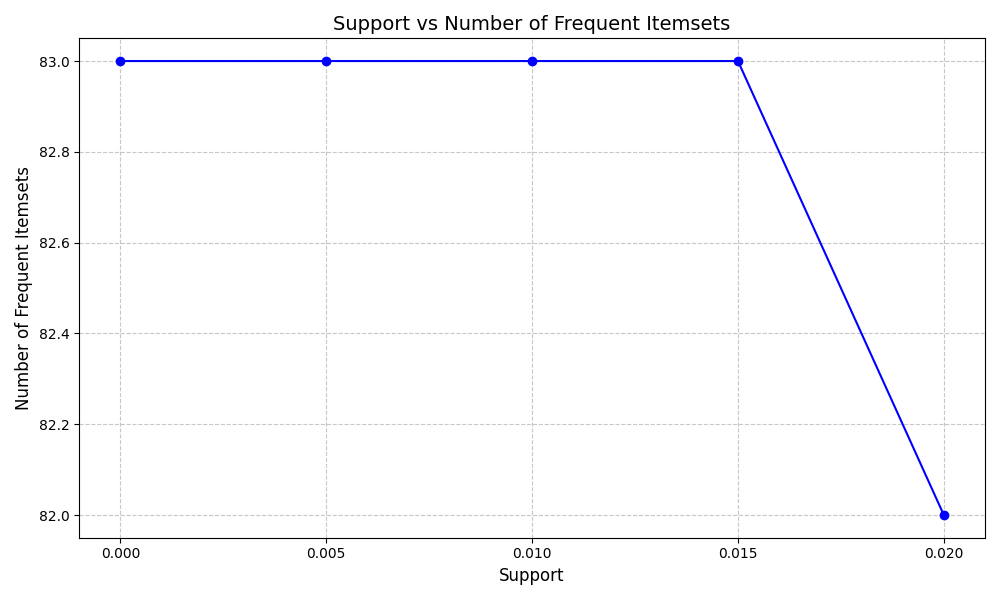
\includegraphics[width=.33\textwidth]{2.png}}
    \subcaptionbox{Step2\label{fig:双图b}}
    {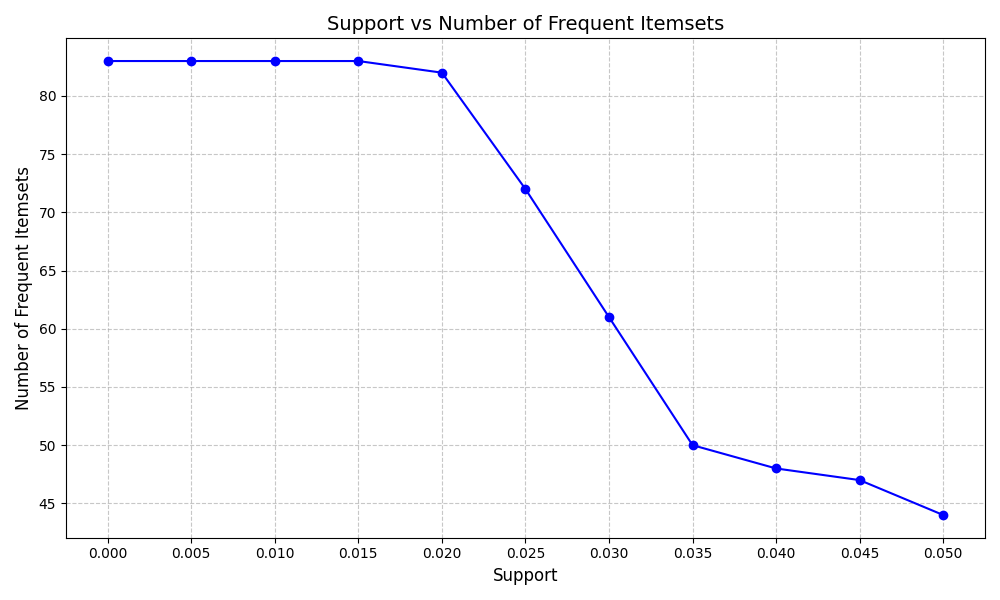
\includegraphics[width=.33\textwidth]{3.png}}
    \subcaptionbox{Step3\label{fig:双图b}}
    {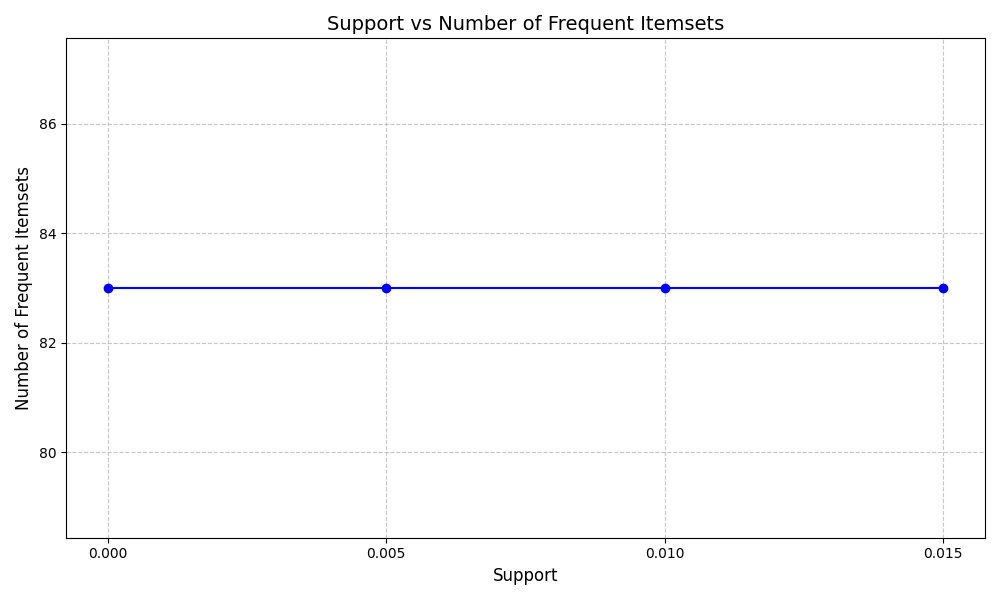
\includegraphics[width=.33\textwidth]{1.png}}
    \caption{支持度-频繁项集数量曲线图}\label{fig:双图}
\end{figure}

不难看出,从开始的拐点较多到最后完成调整后拐点几乎不存在,证明了调整的合理性。
\par

\subsubsection{逐层生成频繁项集}
\textbf{第1层:}生成所有单个项(如 “健康美容”“电子钱包”)的候选集,计算支持度,保留满足阈值的频繁 1 项集。
\par
从此,
逐层生成频繁项集到第k项。即若频繁 2 项集为 {健康美容,电子钱包} 和 {电子钱包,会员},则组合生成候选 3 项集 {健康美容,电子钱包,会员},验证其支持度是否达标。

\subsubsection{基于置信度与提升度筛选有效规则}
\par
\textbf{置信度:}表示在包含前项的交易中,同时包含后项的概率,公式为:
\begin{equation}
\label{eq:公式1}
Confidence(X→Y) = \frac{Support(X\cap Y)}{Support(X)},
\end{equation}

其中,最小置信度确定为:

\par
\textbf{提升度:}提升度是衡量前项和后项之间的关联强度,其公式为:
\begin{equation}
\label{eq:公式1}
Lift(X→Y) = \frac{Confidence(X→Y)}{Support(Y)},
\end{equation}
上述公式中,当Lift>1时,说明X和Y正相关,规则具有实际意义。



\subsection{模型求解}

\subsubsection {问题1.1的求解}
\par
题目要求通过挖掘附件一中的各个指标,
计算各个店的不同指标的统计分布。
在指标选取方面,我们选择销售额、商品单价、商品偏好、性别分布、会员情况、毛利率、评分等七个指标,
在纵向对比不同店之间各个数据的差异,在横向比较店内部不同指标的差别,可视化展示如下图:
\begin{figure}[H]
\centering
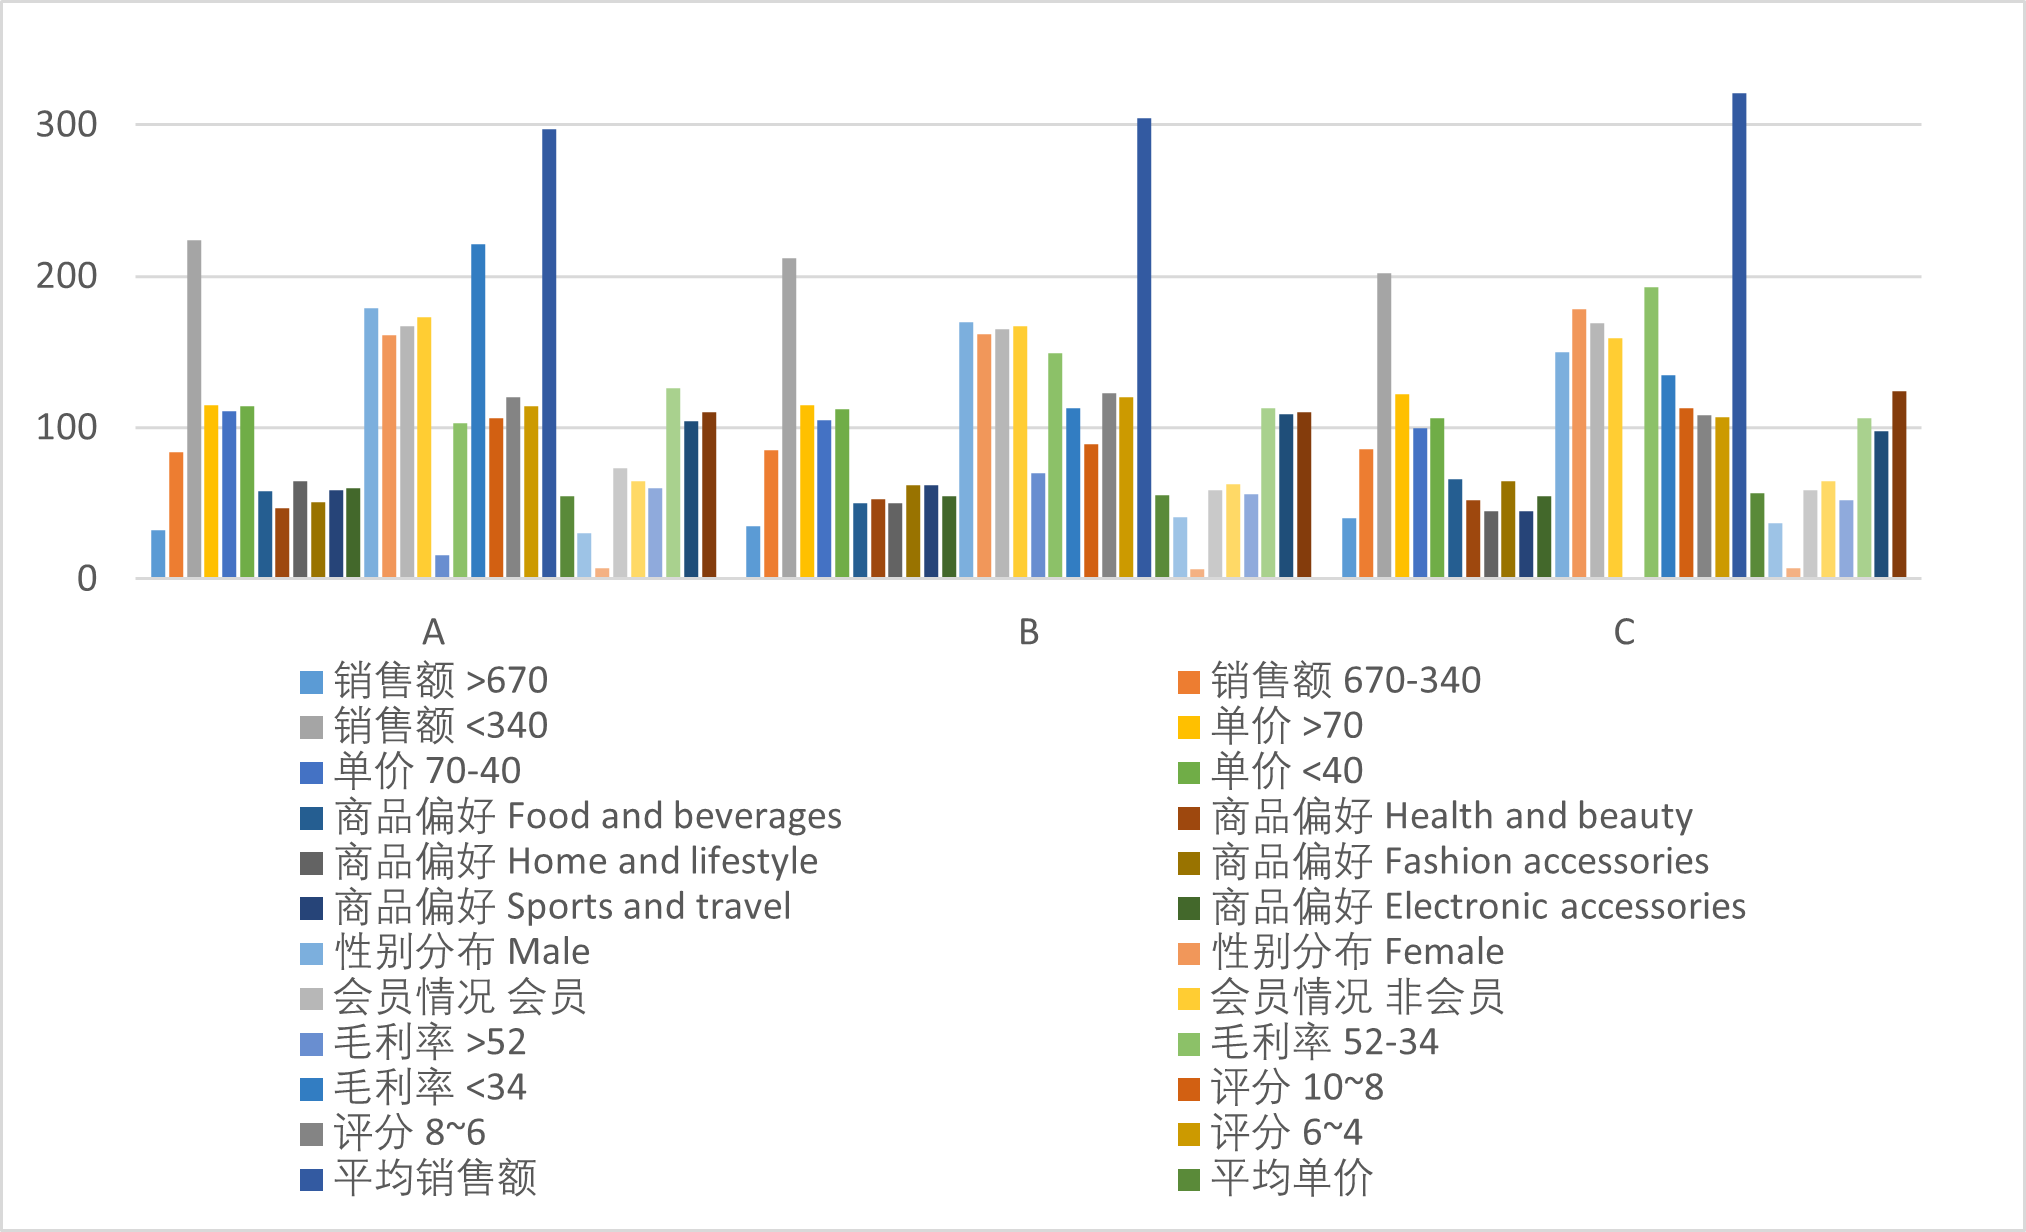
\includegraphics[width=0.8\textwidth]{1.1.png}
\caption{问题1.1可视化展示}
\label{fig:单图}
\end{figure}

\par 

\begin{itemize}[itemindent=2em]
\item 销售额
\par
总体上,我们在销售额方面,将所有商品销售能力划分成高、中、低三种。
划分方式上,我们的划分依据是不同店中各个商品单价最高值均分为三等分,
依次作为分界节点。
其中,在高、中和中、低销售能力商品分割上,小组分别选取了670、370元作为分界线。

\begin{table}[H]
    \captionsetup{font={small,bf,stretch=0.5},justification=raggedright}
    \caption{销售额的统计分布}%\label{tab:001} 、 
    \centering
    \fontsize{12}{14}\selectfont   
    \begin{tabular}{ccccc}
        \toprule[1.5pt]
        店分布 & $>670$ & $340-670$ & $<340$ \\
        \midrule[1pt]
        A & 32(9.4\%) & 84(25.7\%) & 224(65.9\%) \\
        B & 35(10.5\%) & 85(25.6\%) & 212(63.9\%) \\
        C & 40(12.2\%) & 86(26.2\%) & 202(61.6\%) \\
        \bottomrule[1.5pt]
    \end{tabular}
\end{table}

上表中,表格内括号数据代表不同店各个销售额段的占比。
不难发现,三个店的不同分段占比几乎相同。
由此可见,我们的划分依据具有可参考价值。
\item 单价
\par

\begin{table}[H]
    \captionsetup{font={small,bf,stretch=0.5},justification=raggedright}
    \caption{单价的统计分布}%\label{tab:001} 、 
    \centering
    \fontsize{12}{14}\selectfont   
    \begin{tabular}{ccccc}
        \toprule[1.5pt]
        店分布 & $>70$ & $40-70$ & $<40$ \\
        \midrule[1pt]
        A & 115(33.8\%) & 111(32.6\%) & 114(33.5\%) \\
        B & 115(34.6\%) & 105(31.6\%) & 112(33.7\%) \\
        C & 122(37.2\%) & 100(30.5\%) & 106(32.3\%) \\
        \bottomrule[1.5pt]
    \end{tabular}
\end{table}

由上表可见,从跨店对比来看,店C对高价商品偏好最强,店A、B相对均衡,而低价商品在各店接受度相近。这可能反映出店C消费能力较强,A、B消费结构更平衡,商家可据此调整市场策略,如在店C侧重推广高价商品,在A、B兼顾各价格区间商品供应。



\item 商品偏好
\par
\begin{table}[H]
    \captionsetup{font={small,bf,stretch=0.5},justification=raggedright}
    \caption{商品偏好的统计分布}
    \centering
    \fontsize{10}{12}\selectfont  % 适当减小字体
    \begin{tabularx}{\textwidth}{CCCCCCC}  % 使用tabularx自动调整列宽
        \toprule[1.5pt]
        店分布 & Food \& beverages & Health \& beauty & Home \& lifestyle & Fashion accessories & Sports \& travel & Electronic accessories \\ 
        \midrule[1pt]
        A & 58(17.6\%) & 47(13.8\%) & 65(19.1\%) & 51(15.0\%) & 59(17.4\%) & 60(17.6\%) \\
        B & 50(15.1\%) & 53(16.0\%) & 50(15.1\%) & 62(18.7\%) & 62(18.7\%) & 55(16.6\%) \\
        C & 66(20.1\%) & 52(15.9\%) & 45(13.7\%) & 65(19.8\%) & 45(13.7\%) & 55(16.8\%) \\ 
        \bottomrule[1.5pt]
    \end{tabularx}
\end{table}

通过对比分析,三店可划分为两类消费模式:店 A 与店 B 构成 “均衡型消费组”,其各品类占比极差分别为 4.1\% 和 3.6\
\%,商品偏好分布相对均匀;店 C 形成 “倾向型消费组”,食品饮料类占比与次高品类
(时尚配饰,19.8\%)的差值达 0.3 个百分点,且家居生活、运动旅行类占比均为 13.7\%,
显著低于其他店。从消费相似性看,店 A 与店 B 的品类占比相关系数达 0.71,
而店 C 与两者的相关性较弱,暗示其消费需求可能受本地生活习惯或收入水平影响。
同时根据恩格尔系数推断,C店的消费能力相对较弱,可能对商品经济发展会产生不利影响。



\item 性别分布
\par
\begin{table}[H]
    \captionsetup{font={small,bf,stretch=0.5},justification=raggedright}
    \caption{性别的统计分布}%\label{tab:001} 、 
    \centering
    \fontsize{12}{14}\selectfont   
    \begin{tabular}{ccccc}
        \toprule[1.5pt]
        店分布 & male & female \\
        \midrule[1pt]
        A & 179(52.6\%) & 161(47.4\%)  \\
        B & 170(51.2\%) & 162(48.8\%)  \\
        C & 150(45.7\%) & 178(54.3\%)  \\
        \bottomrule[1.5pt]
    \end{tabular}
\end{table}
\par
上表可知,在A、B两店中,男性的平均购买水平要高于女性,而在C店中,则恰恰相反,
女性的购买水平要远高于男性。
因此,在A、B两店中可以将产品导向略微偏向男性,而C店中可以偏向女性。





\item 会员情况
\par
\begin{table}[H]
    \captionsetup{font={small,bf,stretch=0.5},justification=raggedright}
    \caption{会员情况的统计分布}%\label{tab:001}  
    \centering
    \fontsize{12}{14}\selectfont   
    \begin{tabular}{ccccc}
        \toprule[1.5pt]
        店分布 & member & normal \\
        \midrule[1pt]
        A & 167(49.1\%) & 173(50.9\%)  \\
        B & 165(49.7\%) & 167(50.3\%)  \\
        C & 169(51.5\%) & 159(48.5\%)  \\
        \bottomrule[1.5pt]
    \end{tabular}
\end{table}
\par
由上表可见,在纵向方向来看,三座店的会员情况大多相同;而在横向方向比较的,店内部的会员与非会员的分布大概平均分布,基本上保持在1:1的关系。




\item 毛利率
\begin{table}[H]
    \captionsetup{font={small,bf,stretch=0.5},justification=raggedright}
    \caption{毛利率的统计分布}%\label{tab:001}  
    \centering
    \fontsize{12}{14}\selectfont   
    \begin{tabular}{ccccc}
        \toprule[1.5pt]
        店分布 & $>52$ & $34-52$ & $<34$ \\
        \midrule[1pt]
        A & 16(4.7\%) &103(30.2\%) & 221(65.0\%) \\
        B & 70(21.1\%) & 149(44.9\%) & 113(34.0\%) \\
        C & 0(0\%) & 193(58.8\%) & 135(41.2\%) \\
        \bottomrule[1.5pt]
    \end{tabular}
\end{table}
由上表可知,C的毛利率最低,而B的毛利率最高。


\item 评分
\begin{table}[H]
    \captionsetup{font={small,bf,stretch=0.5},justification=raggedright}
    \caption{评分的统计分布}%\label{tab:001}  
    \centering
    \fontsize{12}{14}\selectfont   
    \begin{tabular}{ccccc}
        \toprule[1.5pt]
        店分布 & $4-6$ & $6-8$ & $8-10$ \\
        \midrule[1pt]
        A & 114(33.5\%) &120(35.3\%) & 106(31.2\%) \\
        B & 120(36.1\%) & 123(37.0\%) & 89(26.8\%) \\
        C & 107(32.6\%) & 108(32.9\%) & 113(34.5\%) \\
        \bottomrule[1.5pt]
    \end{tabular}
\end{table}
\par
由上表可知,B店的平均得分为三个店内最高,而C店则相对评分略低。
根据上述表格综合分析,可知由于C店的对商品要求较高,需要引进搞性价比商品或者搞质量商品;
而相对而言,B店评分较高,可以减少相关改动。



\item 平均销售额、平均单价、平均毛利率和平均评分
\begin{table}[H]
    \captionsetup{font={small,bf,stretch=0.5},justification=raggedright}
    \caption{平均销售额、平均单价、平均毛利率、平均评分的统计分布}%\label{tab:001}  
    \centering
    \fontsize{12}{14}\selectfont   
    \begin{tabular}{ccccc}
        \toprule[1.5pt]
        店分布 & 平均销售额 & 平均单价 & 平均毛利率 & 平均评分 \\
        \midrule[1pt]
        A & 297.48 & 54.78 & 30.17 & 7.03 \\
        B &  304.64& 55.66 & 40.84 & 6.82 \\
        C & 321.05 & 56.61 & 36.78 & 7.07 \\
        \bottomrule[1.5pt]
    \end{tabular}
\end{table}
由上表可见,通过指标关联性分析,店 A 与 B 可划分为 “均衡型消费组”:两者销售额与单价差距微小,毛利率与评分的离散程度较低(毛利率极差 10.67,评分极差 0.21),表明消费结构与市场反馈相对稳定。店 C 则形成 “高值倾向型消费组”:销售额与单价的双高特征显著(Z 得分分别为 1.27 和 1.15),但毛利率低于店 B,可能因高价商品成本结构不同或促销策略差异所致。从指标相关性看,店 A 与 B 的销售额 - 单价相关系数达 0.92,而店 C 的毛利率 - 评分相关性更强(ρ=0.81),暗示其消费群体更关注性价比与服务体验的平衡,而 A、B 可能更依赖商品价格驱动消费。该差异或与店 C 的高收入群体占比、商品供给层级(如高端品类更多)相关,而 A、B 的消费生态更偏向大众市场均衡发展。

\item 不同店的消费时段
\par
通过对excel中的数据进行统一分析,我们可以得到:
\begin{figure}[H]
\centering
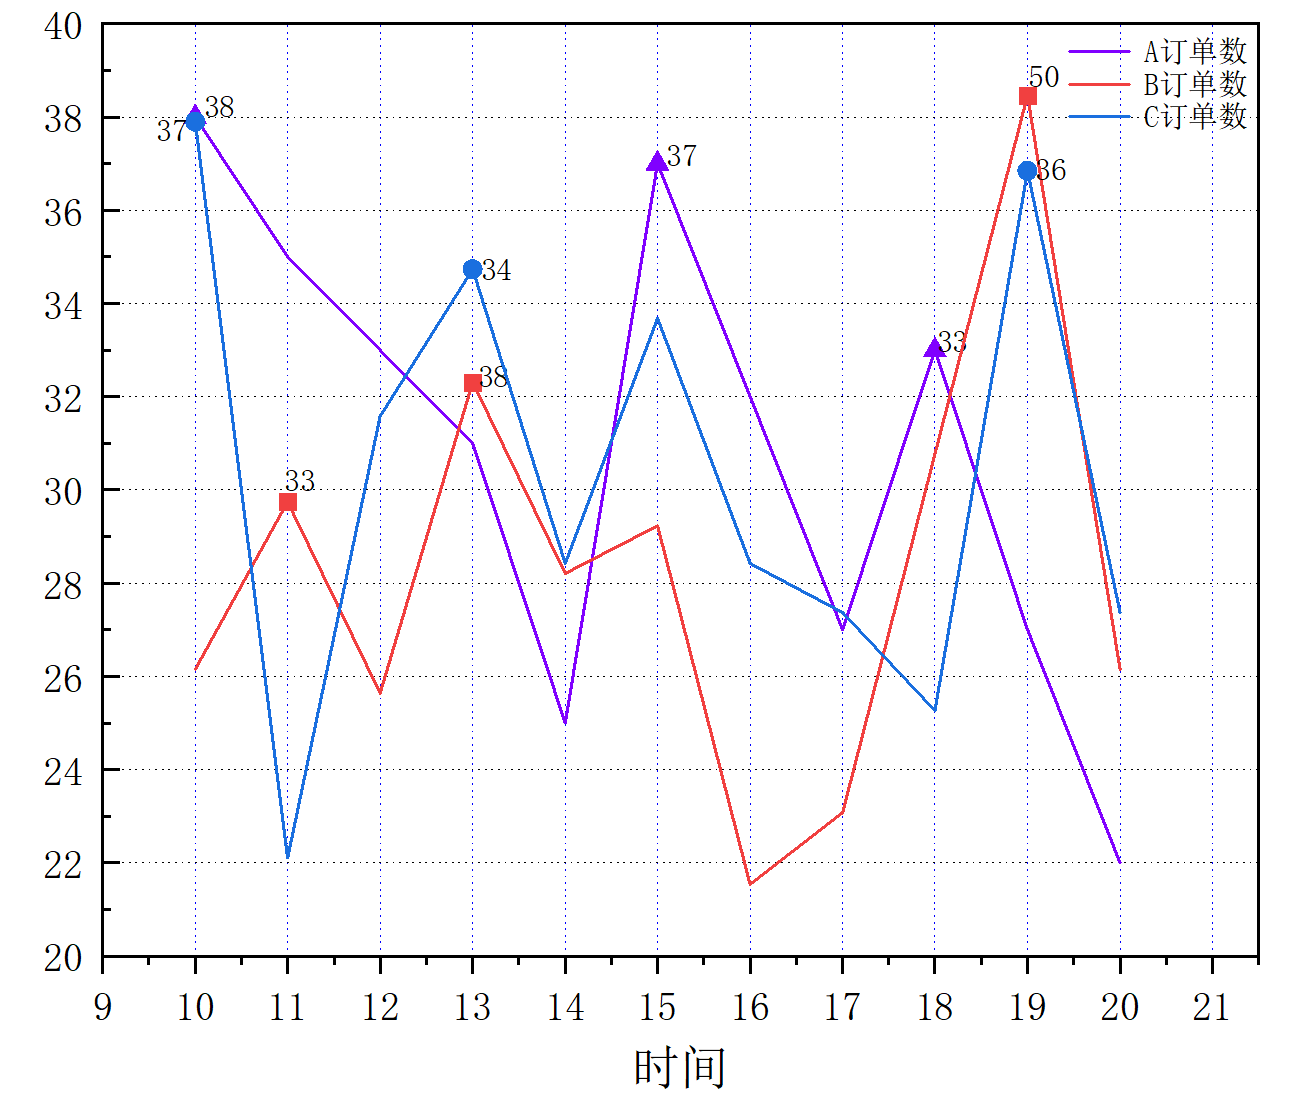
\includegraphics[width=0.5\textwidth]{cycle.png}
\caption{各店订单随时间折线图}
\label{fig:单图}
\end{figure}

由上图可知,A店订单在10点、15点和19点分别达到早、中和晚三个高峰,
B店订单在11点、13点和18点分别达到早、中和晚三个高峰,
C店订单在10点、13点和19点分别达到早、中和晚三个高峰。
\item 不同店在付款选择上的差异
\par
\begin{table}[H]
    \captionsetup{font={small,bf,stretch=0.5},justification=raggedright}
    \caption{支付方式的统计分布}%\label{tab:001}  
    \centering
    \fontsize{12}{14}\selectfont   
    \begin{tabular}{ccccc}
        \toprule[1.5pt]
        店分布 & 电子钱包 & 信用卡 & 现金 \\
        \midrule[1pt]
        A & 126 &104 & 110 \\
        B & 113 & 109 & 110 \\
        C & 106 & 98 & 124 \\
        \bottomrule[1.5pt]
    \end{tabular}
\end{table}

由上表可见,纵向比较来看,A店使用电子钱包相对较多,而B店使用信用卡相对较多,而C店相对使用现金较多。
横向比较来看,在店内部,A店和B店三种支付方式基本呈现1:1:1的分布,而C店则使用现金付款方式较多,而信用卡使用相对较少。


\end{itemize}

\subsubsection {问题1.2的求解}
\begin{figure}[H]
\centering
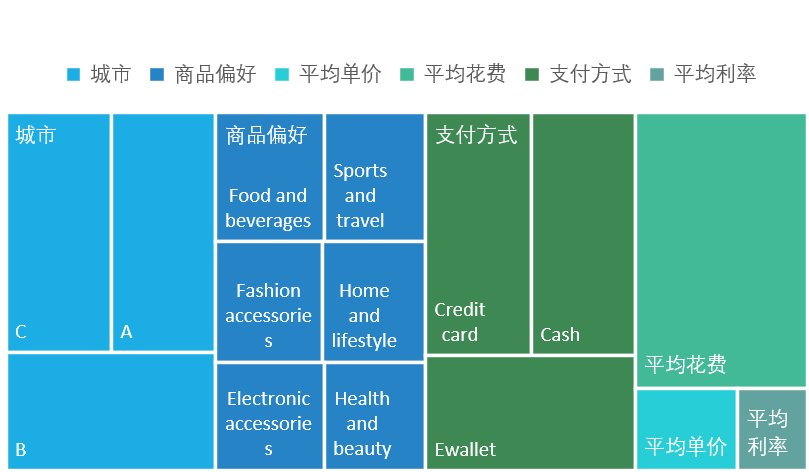
\includegraphics[width=0.8\textwidth]{1.2.png}
\caption{问题1.2可视化展示}
\label{fig:单图}
\end{figure}
\begin{table}[H]
    \captionsetup{font={small,bf,stretch=0.5},justification=raggedright}
    \caption{会员与非会员消费时间中位数、消费数量、平均单价对比}%\label{tab:001}  
    \centering
    \fontsize{12}{14}\selectfont 
\begin{tabular}{cccccc}
\toprule[1.5pt]
    \multirow{2}{*}{Customer type}& \multirow{2}{*}{时间中位数} & \multicolumn{3}{l}{店消费数量} & \multirow{2}{*}{平均单价} \\ \cline{3-5}
    &                        & A      & B     & C     &                       \\ \midrule[1pt]
Member  & 15:24                  & 167    & 165   & 169   & 56.21                 \\
Normal & 15:19                  & 173    & 167   & 159   & 55.14                 \\ \bottomrule[1.5pt]
\end{tabular}
\end{table}
从时间中位数看,会员消费时间集中在 15:24,较非会员(15:19)延后 5 分钟,在这方面两者并无太大差异。
消费数量方面,会员在 A、B、C 三店的消费数量分别为 167、165、169,非会员为 173、167、159,除店 C 外,非会员消费数量略高于会员,但整体差距较小(最大差值 8,占比约 4.7\%)。
值得注意的是,店 C 的会员消费数量(169)反超非会员(159),或暗示该店会员忠诚度更高。
\par
会员平均单价为 56.21 元,较非会员(55.14 元)高出 1.9\%,虽差距绝对值较小,但反映会员群体可能更倾向于选购中高端商品或对价格敏感度较低。结合店维度,三店的会员与非会员单价均呈现递增趋势(A<B<C),与店经济发展水平可能存在相关性。
从消费模式看,会员的消费时间延后、单价略高的特征,或与其消费习惯(如享受会员专属时段服务)或消费能力较强有关,而非会员更注重消费频次与性价比,建议针对会员群体优化晚间服务或推出高端商品套餐,提升消费体验与客单价。

\begin{table}[H]
    \captionsetup{font={small,bf,stretch=0.5},justification=raggedright}
    \caption{会员与非会员商品偏好的统计分布(消费数量,单位:件)}
    \centering
    \fontsize{12}{14}\selectfont 
    \begin{tabular}{lcccccc}
        \toprule[1.5pt]
        \textbf{用户类型} & \textbf{食品饮料} & \textbf{健康美容} & \textbf{家居生活} & \textbf{时尚配饰} & \textbf{运动旅行} & \textbf{电子配件} \\
        \midrule[1pt]
        会员               & 94               & 73               & 83               & 86                & 87               & 78                 \\
        非会员             & 80               & 79               & 77               & 92                & 79               & 92                 \\
        \bottomrule[1.5pt]
    \end{tabular}
\end{table}
对比发现,会员在食品饮料类的消费数量比非会员高出 17.5\%,或因会员专属优惠拉动刚需消费;
非会员在时尚配饰与电子配件上的消费分别较会员高出 6.9\% 和 17.9\%,更倾向潮流商品。健康美容和运动旅行品类中,
两者消费数量差异较小。基于此,建议针对会员加强刚需商品的捆绑营销,对非会员则围绕潮流商品设计组合优惠,以提升消费吸引力。
\par
同时根据TOPSIS模型,我们得到了相关贡献度,如下表:
\begin{table}[H]
    \captionsetup{font={small,bf,stretch=0.5},justification=raggedright}
    \caption{会员与非会员的贡献度比较}%\label{tab:001}  
    \centering
    \fontsize{12}{14}\selectfont   
    \begin{tabular}{ccccc}
        \toprule[1.5pt]
        顾客分布 & 贡献度 & 贡献度占比  \\
        \midrule[1pt]
        会员 & 34.38 &52.3\%\\
        非会员 & 31.38 & 47.7\% \\
        \bottomrule[1.5pt]
    \end{tabular}
\end{table}
\par
由上表可知,会员的贡献度要大于非会员。

\subsubsection {问题1.3的求解}

\begin{table}[H]
    \captionsetup{font={small,bf,stretch=0.5},justification=raggedright}
    \caption{高频购买组合}%\label{tab:001} 、 
    \centering
    \fontsize{12}{14}\selectfont   
    \begin{tabular}{ccccccccc}
        \toprule[1.5pt]
        1 & 2 & 3 & 4 \\
        \midrule[1pt]
        Credit card & Sports and travel & Member & 67.9\% \\
        Cash & Fashion accessories & Normal & 59.6\% \\
        Cash & Home and lifestyle & Member & 58.8\% \\
        Health and beauty&Ewallet & Normal& 58.5\% \\
        Cash& Food and beverages& Member& 57.9\% \\
        Cash& Electronic accessories& Normal& 56.3\% \\
        Ewallet& Home and lifestyle& Normal& 56.3\% \\
        Credit card& Home and lifestyle& Member& 55.6\% \\
        Ewallet& Sports and travel& Normal& 55.6\% \\
        Credit card& Member& *& 55.3\% \\
        \bottomrule[1.5pt]
    \end{tabular}
\end{table}

\par
上表中,表示了前10的购买组合,依次按照其对应的置信度,即该组合更加具有落地价值。
其中,运动旅游+信用卡+会员的组合的置信度最高,即最具有实际意义。



\subsubsection {问题1.4的求解}

\begin{figure}[H]
\centering
\subcaptionbox{Fashion accessories\label{fig:双图a}}
{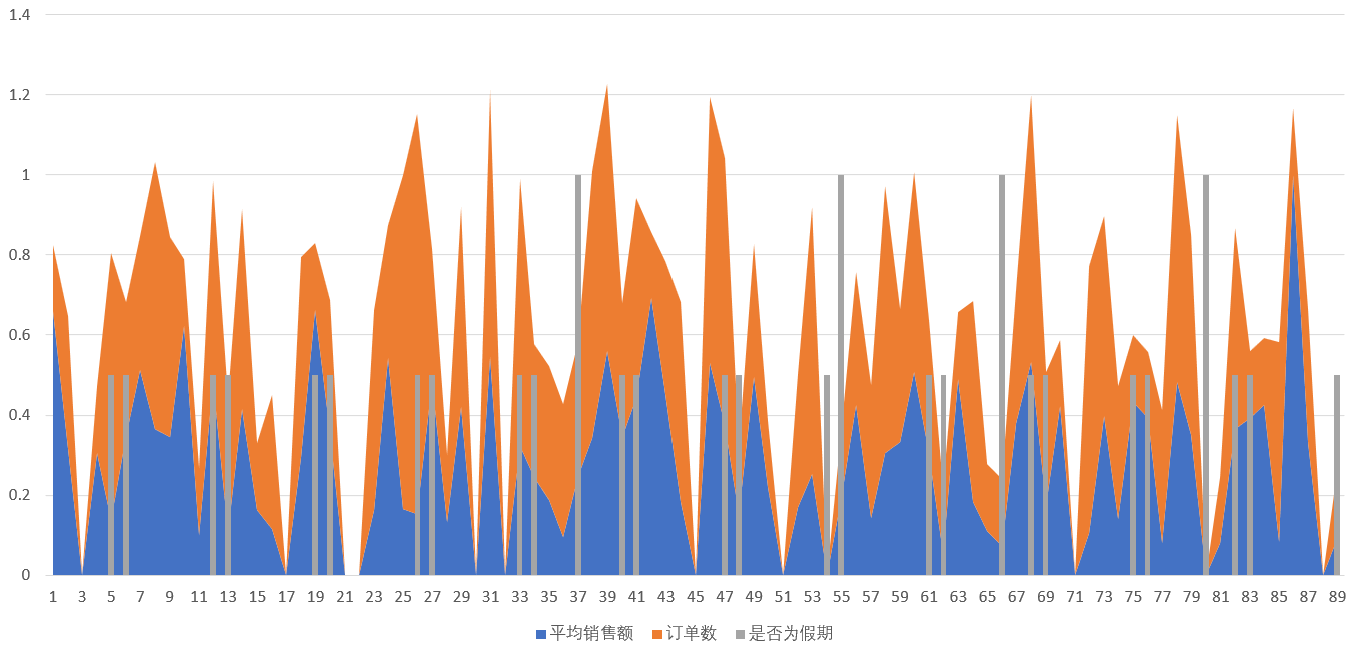
\includegraphics[width=.4\textwidth]{fashion.png}}
\subcaptionbox{Food and beverages\label{fig:双图b}}
{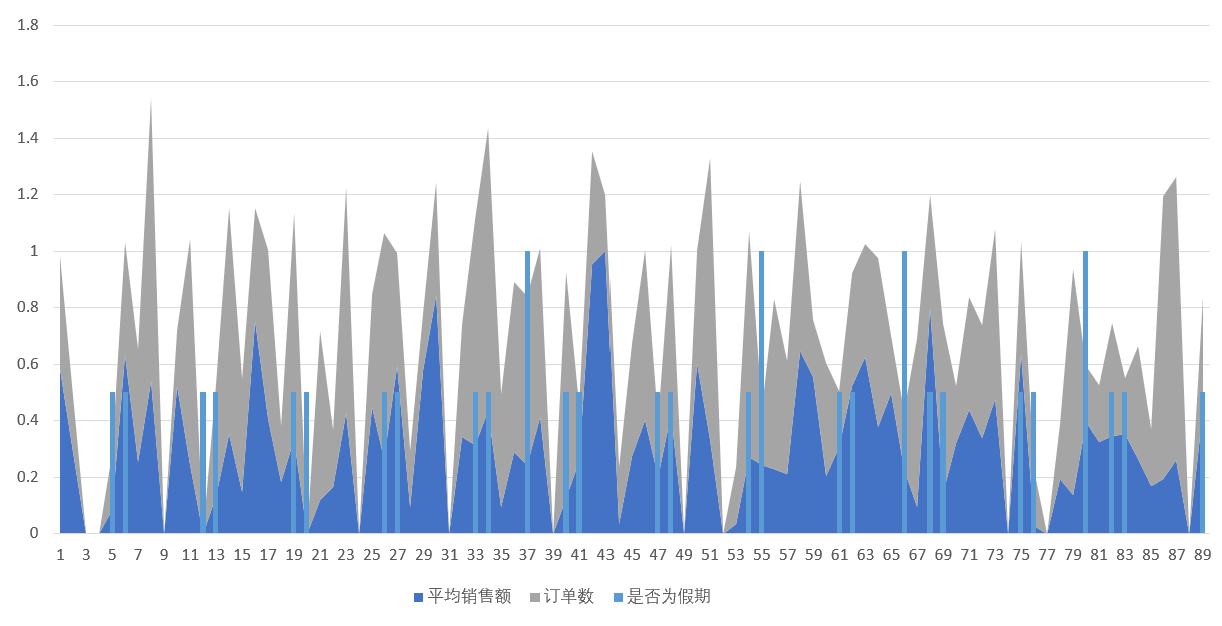
\includegraphics[width=.4\textwidth]{food.png}}
\caption{Fashion accessories和Food and beverages销售堆积图}\label{fig:双图}
\end{figure} 

\begin{figure}[H]
\centering
\subcaptionbox{Health and beauty\label{fig:双图a}}
{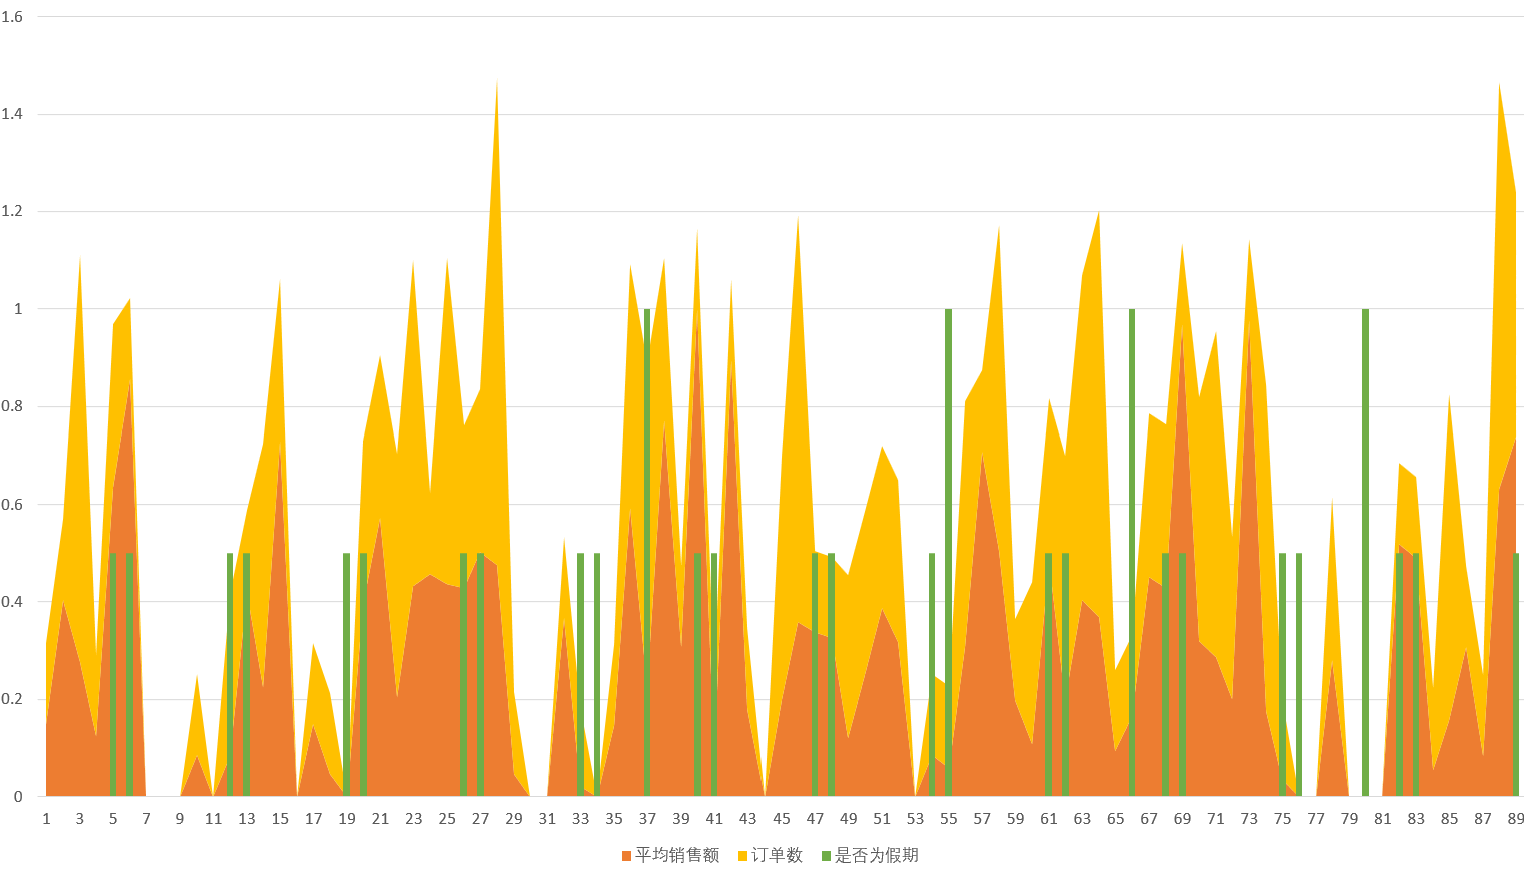
\includegraphics[width=.4\textwidth]{health.png}}
\subcaptionbox{Home and lifestyle\label{fig:双图b}}
{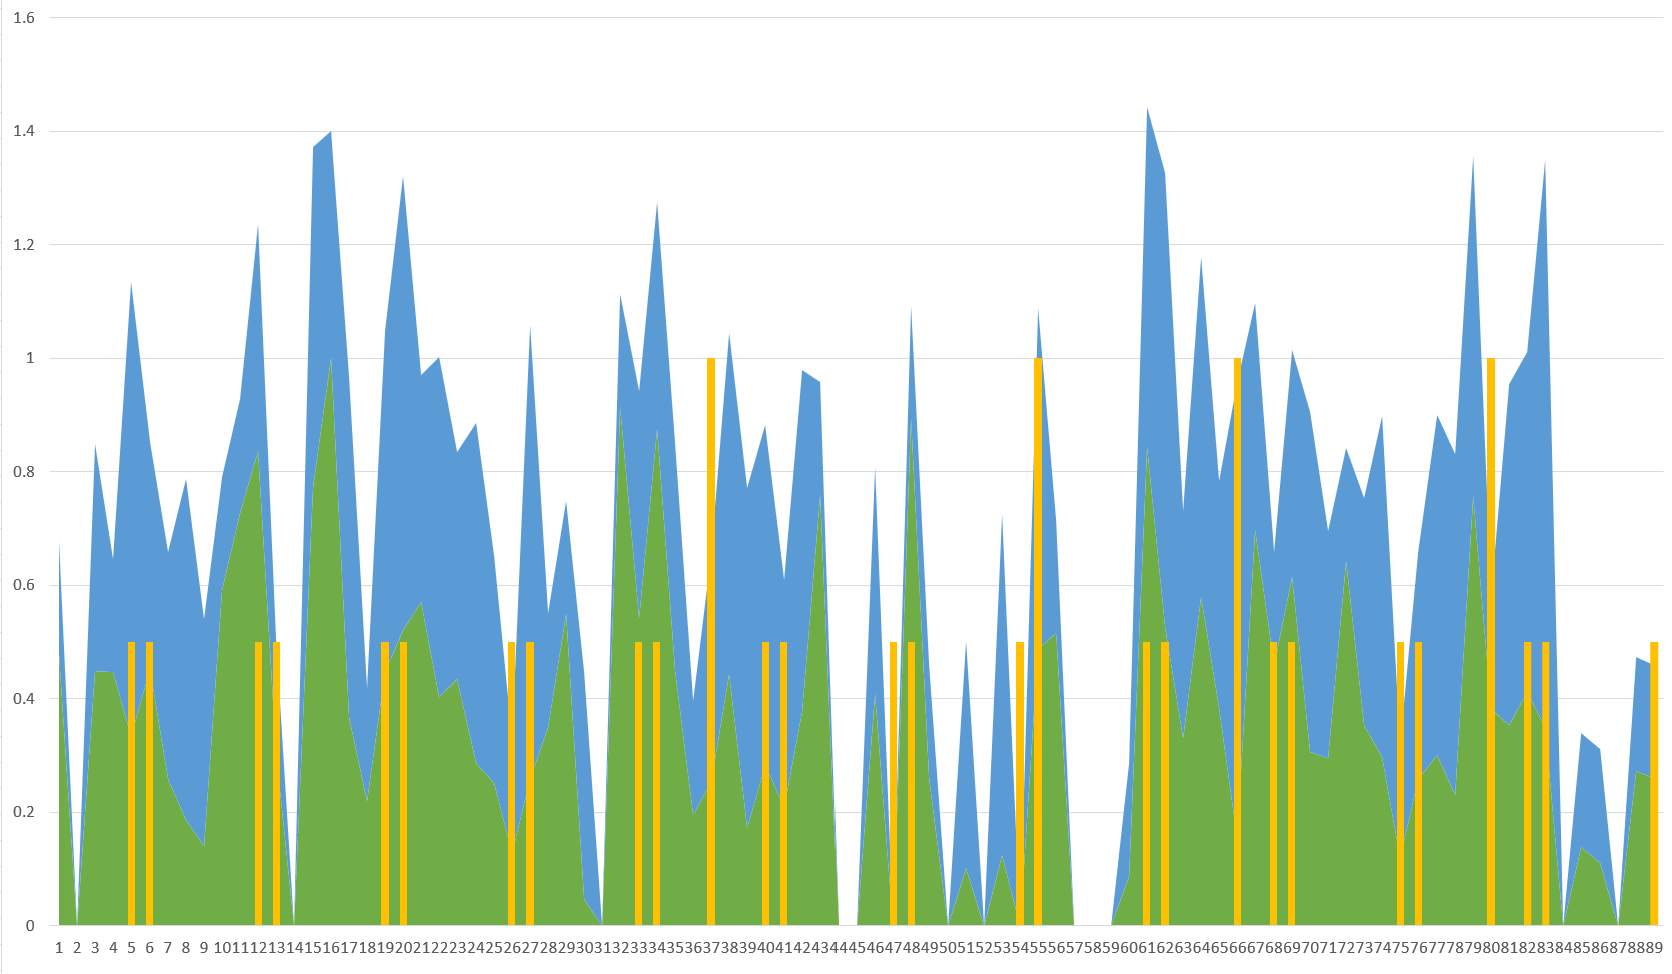
\includegraphics[width=.4\textwidth]{home.png}}
\caption{Health and beauty和Home and lifestyle销售堆积图}\label{fig:双图}
\end{figure} 

\begin{figure}[H]
\centering
\subcaptionbox{Electronic accessories\label{fig:双图a}}
{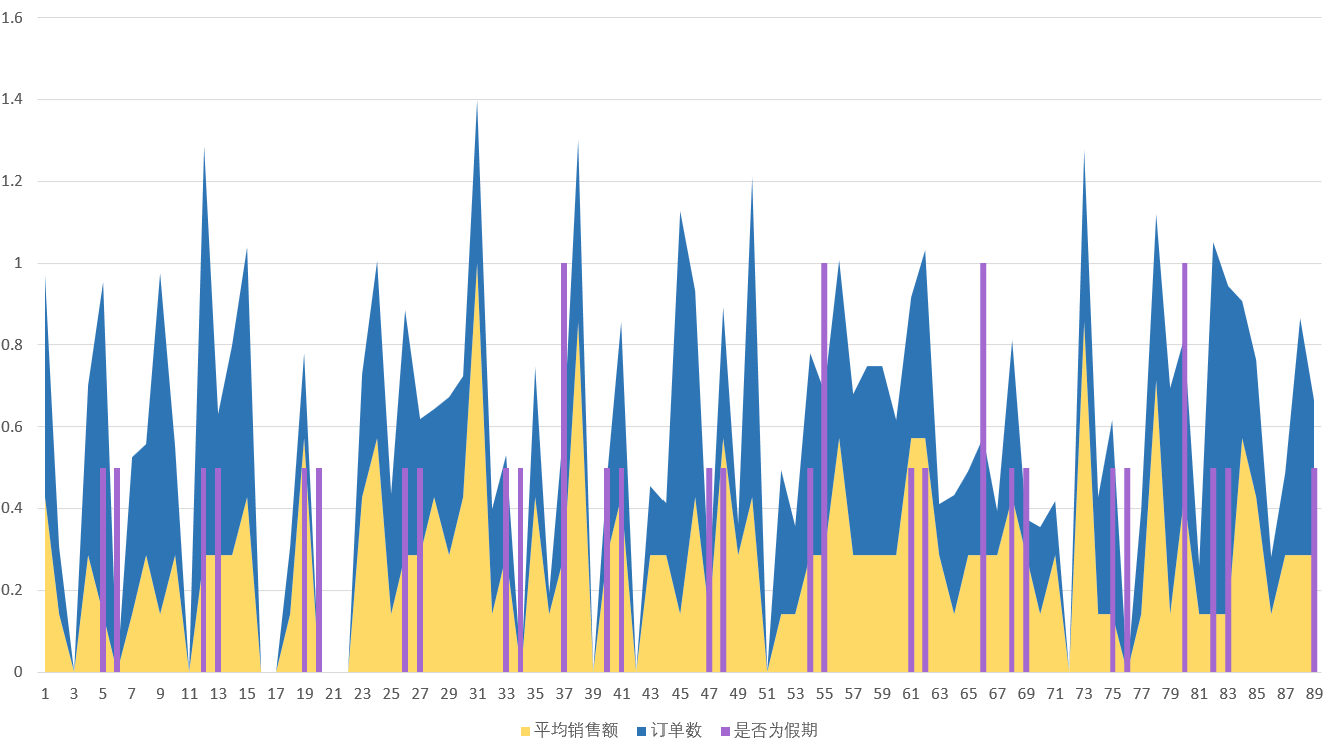
\includegraphics[width=.4\textwidth]{electronic.png}}
\subcaptionbox{Sports and travel\label{fig:双图b}}
{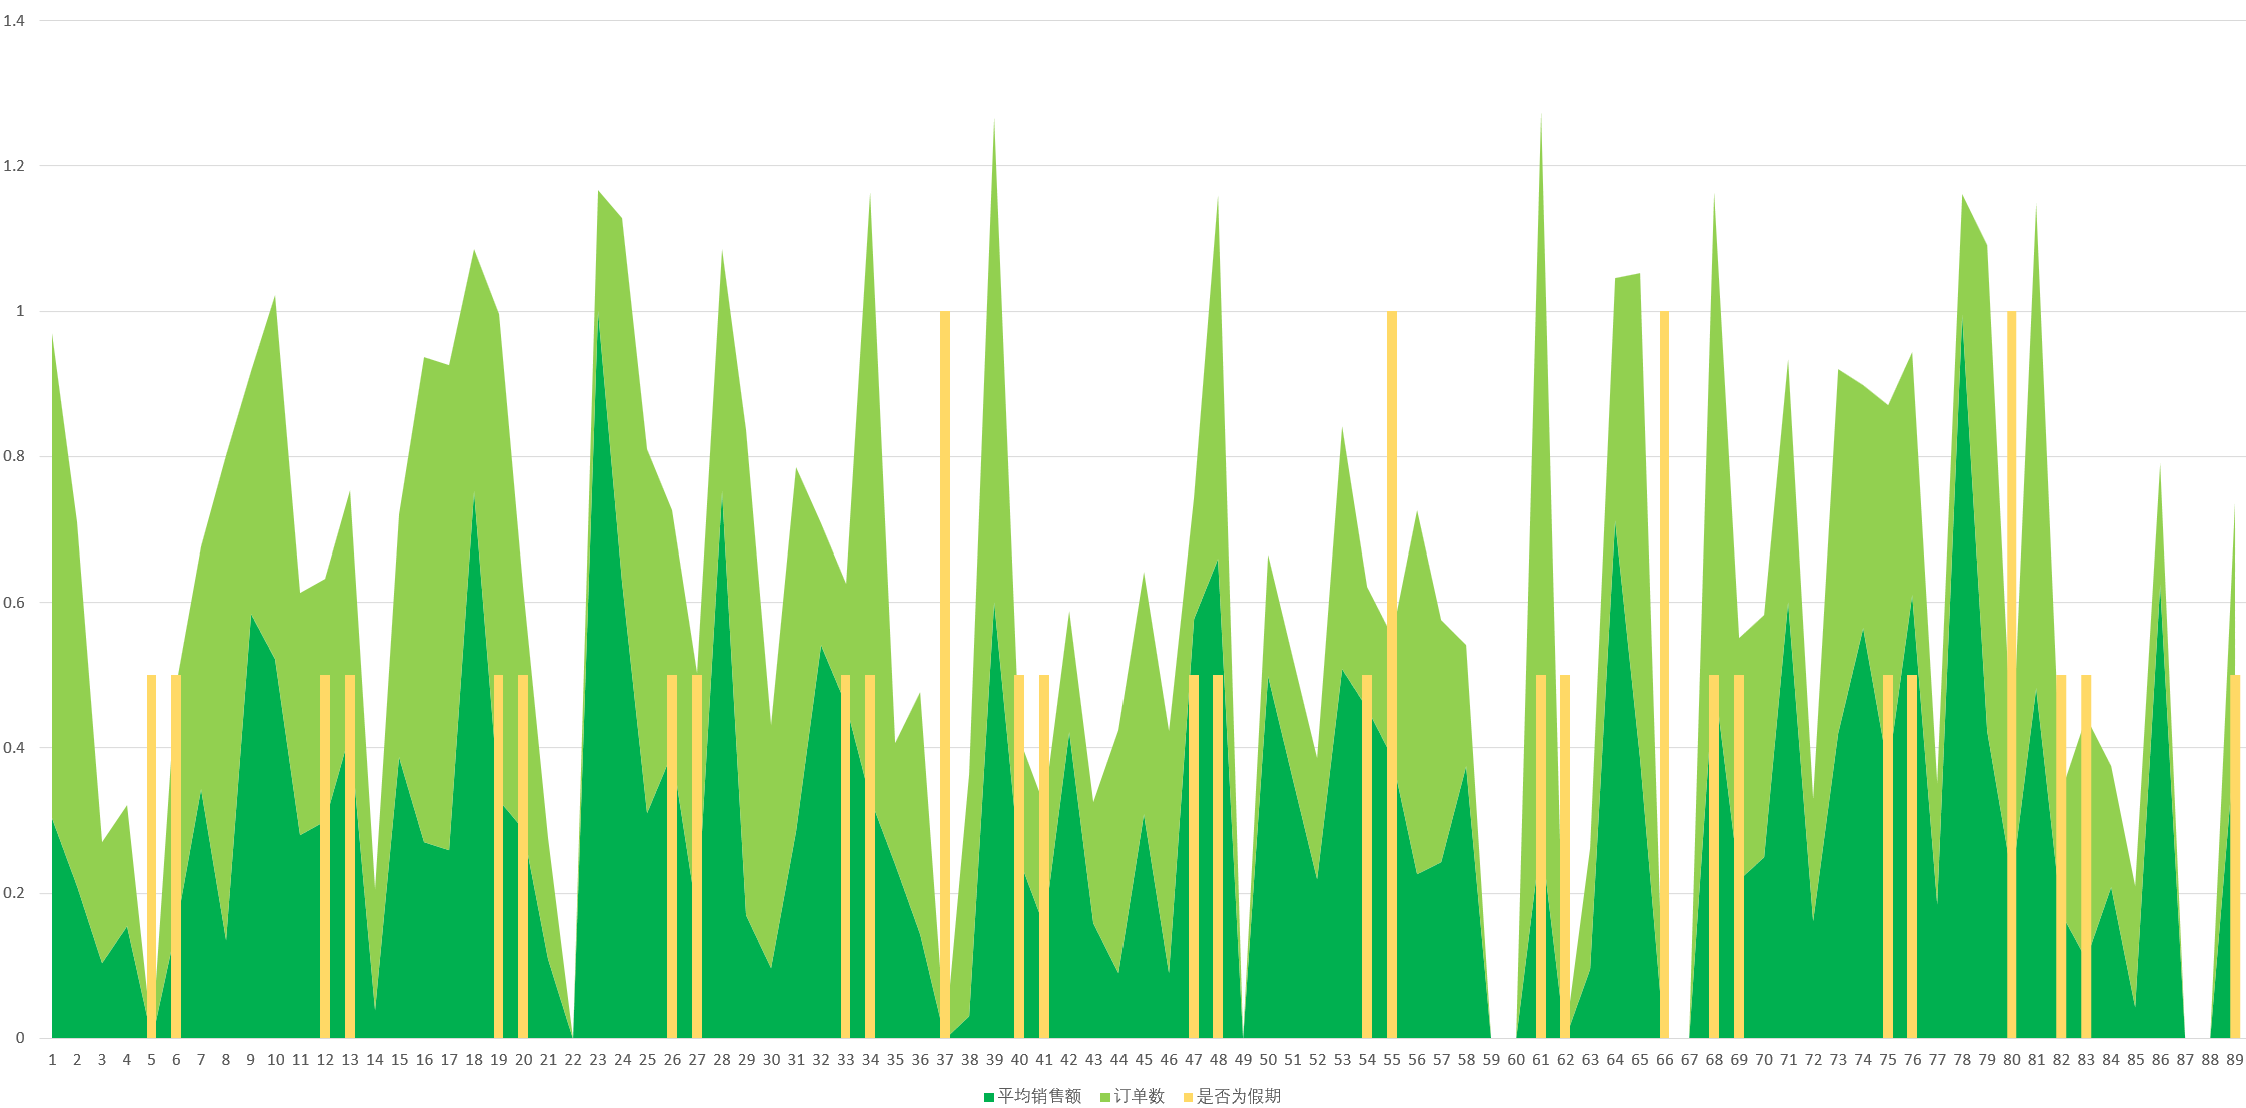
\includegraphics[width=.4\textwidth]{sport.png}}
\caption{Electronic accessories和Sports and travel销售堆积图}\label{fig:双图}
\end{figure} 

由上图可知,其中所有商品在大多数周末达到峰值。但是存在一定的不确定性,例如:Fashion accessories大部分为周末假期的平均销售额有上升趋势,
但在53-55天(在上述图片中,横坐标的时间代表相对1月7日的天数加1)时,出现一定反差。

%%%%%%%%%%%%%%%%%%%%%%%%%%%%%%%%%%%%%%%%%%%%%%%%%%%%%%%%%%%%% 

\section{问题二的模型的建立和求解}
\subsection{数据预处理}

\subsubsection{KS正态性检验}\par
在数据与处理方面,本题前半段分析各个指标之间的相关性,需要验证其是否符合正态性,以为后续操作选择更优计算方式和数学模型,因此在本步小组使用KS正态性检验。\upcite{hanusz2016shapiro}

\textbf{Step1}计算样本统计量
\par
样本均值:
\begin{equation}
\label{eq:公式1}
 \hat{\mu} = \frac{1}{n} \sum_{i=1}^n x_i 
\end{equation}
\par


样本标准差:
\begin{equation}
\label{eq:公式1}
\hat{\sigma} = \sqrt{\frac{1}{n-1} \sum_{i=1}^n (x_i - \hat{\mu})^2} 
\end{equation}
\par

\textbf{Step2}标准化样本
\par
将样本转换为标准正态分布的形式:
\begin{equation}
\label{eq:公式1}
z_i = \frac{x_i - \hat{\mu}}{\hat{\sigma}}
\end{equation}

\par

\textbf{Step3}计算经验分布函数(ECDF)和理论分布函数(CDF)
\par
\begin{itemize}[itemindent=2em]

\item 经验分布函数:将标准化后的样本排序为:
\begin{equation}
\label{eq:公式1}
 z_1 \leq z_2 \leq \dots \leq z_n 
\end{equation}
\par
则:
\begin{equation}
\label{eq:公式1}
F_n(z_i) = \frac{i}{n} \quad (\text{第 } i \text{ 个样本的经验分布值})
\end{equation}
\par
\item 理论正态分布的累积分布函数:

\begin{equation}
\label{eq:公式1}
\Phi(z_i) = \frac{1}{\sqrt{2\pi}} \int_{-\infty}^{z_i} e^{-\frac{t^2}{2}} dt
\end{equation}
\par
\end{itemize}

\textbf{Step4}计算KS统计量
\par
\begin{equation}
\label{eq:公式1}
D = \max_{1 \leq i \leq n} \left| F_n(z_i) - \Phi(z_i) \right|
\end{equation}
\par
即经验分布与理论正态分布的最大垂直距离。

\par

\textbf{Step5}显著性检验
\par
根据样本量n和显著水平$\alpha$ (如0.05),查KS检验临界值表或通过公式近似计算临界值  $D_{\alpha}$ 。若  D > $D_{\alpha}$ ,则拒绝原假设(样本不服从正态分布);否则不拒绝。

\textbf{Step6}查找对应的临界值并作出比较
\par
本问中,临界值取0.05,可视化结果如下图:

\begin{figure}[H]
\centering
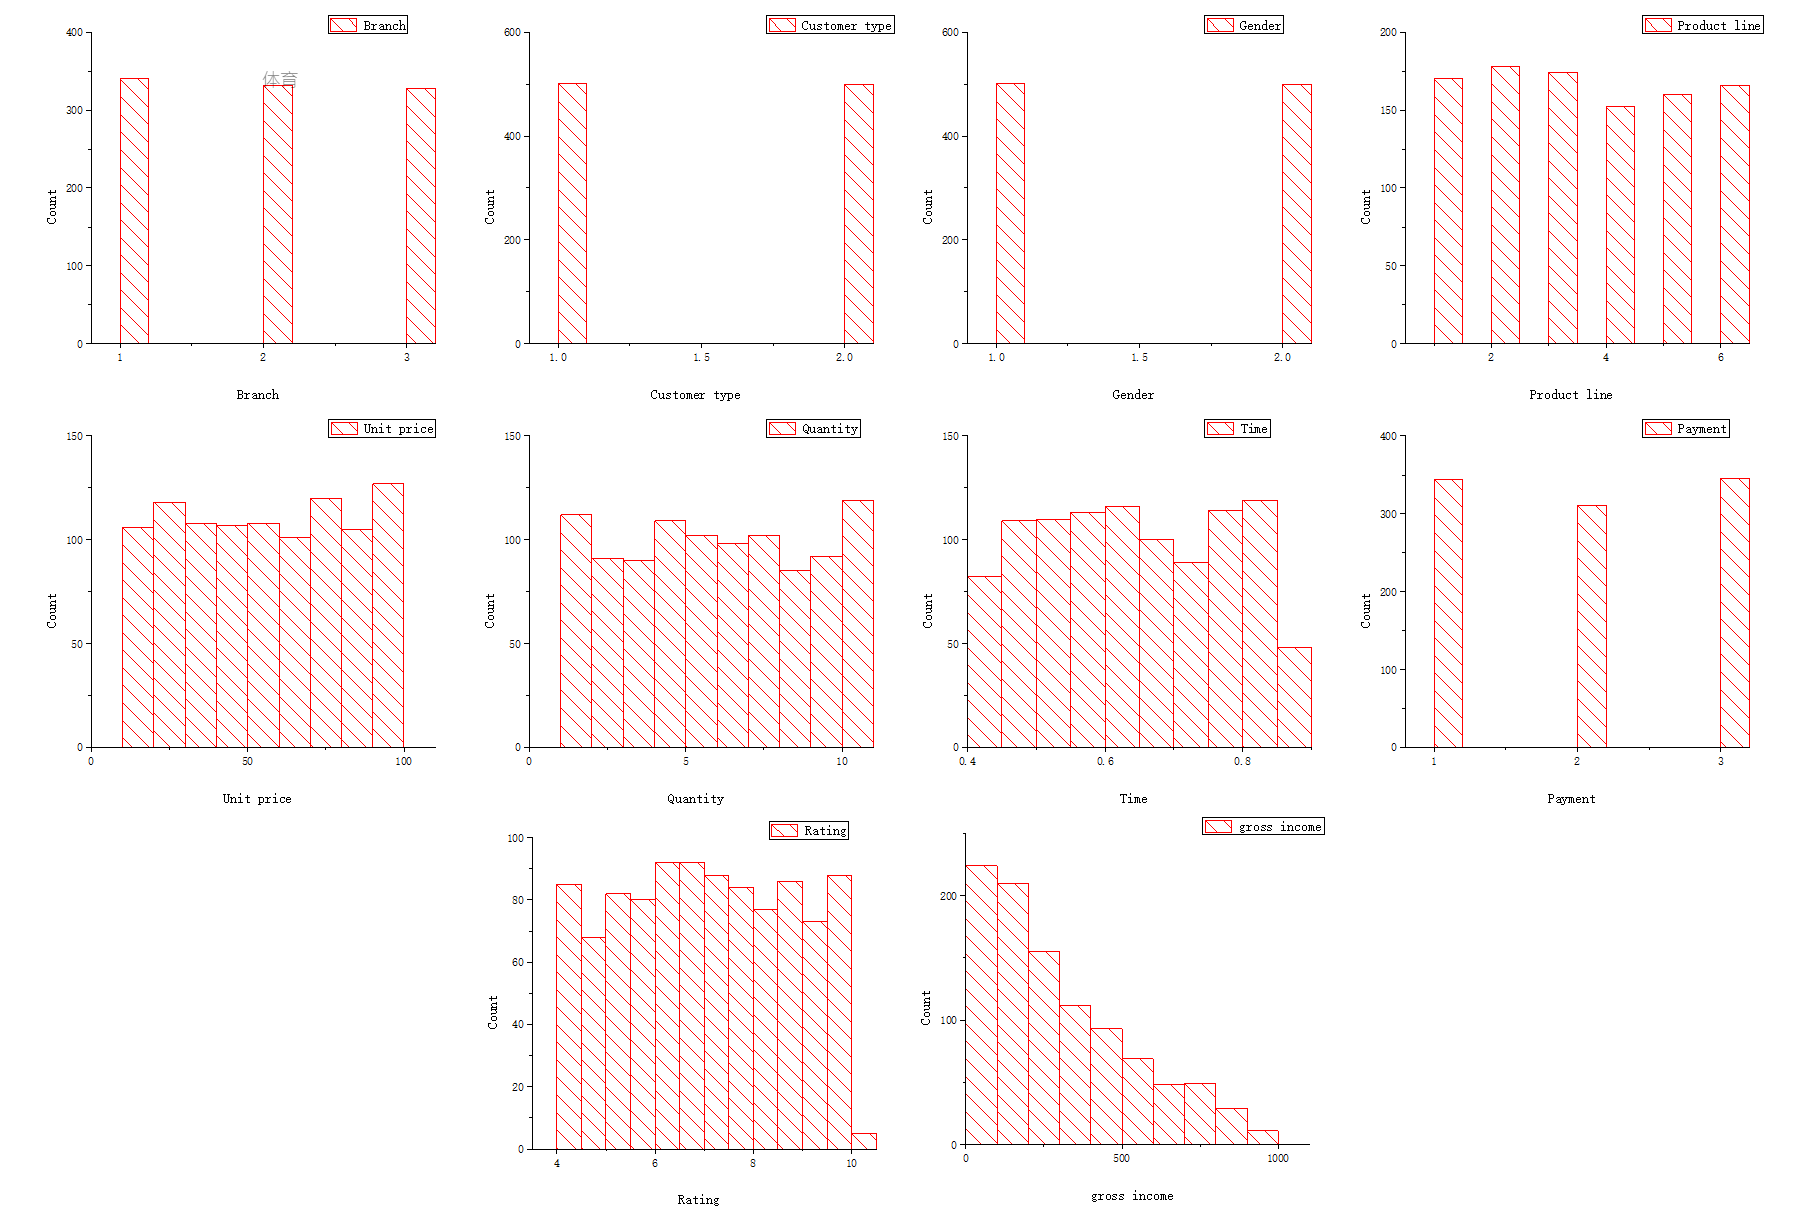
\includegraphics[width=0.75\textwidth]{SW正态性检验直方集合图.png}
\caption{KS正态性检验直方集合图}
\label{fig:单图}
\end{figure}

\begin{table}[H]
    \captionsetup{
        font={small, bf},
        justification=raggedright,
        singlelinecheck=false
    }
    \caption{\centering{正态性检验数据表}}
    \label{tab:gross_margin_prediction}
    \centering
    \fontsize{5}{7}\selectfont % 调整字体大小为7pt,行高9pt
    \begin{tabularx}{\textwidth}{CCCCCCCCCCCC} % 修正为11列
        \toprule[1.5pt]
        数据 & Branch & Customer type & Gender & Product line & Unit price & Quantity & Time & Payment & Rating & gross income \\
        \midrule[1pt]
        p值 & <0.0001 & <0.0001 & <0.0001 & <0.0001 & $2.15\times 10^{-4}$ & <0.0001 & <0.0001 & <0.0001 & $2.56\times 10^{-4}$ & <0.0001 \\
        \bottomrule[1.5pt]
    \end{tabularx}
\end{table}



由上图及上表可知,KS正态性检验数据均小于0.05,数据不成正态性,因此后续分析采用斯皮尔曼分析方式。

\subsubsection{傅里叶变换设计低通滤波}
由于本题综合数据样本较多,数据起伏较大。通过傅里叶变换对数据进行平滑处理,有助于后续的模型建立。


\textbf{Step1}定义输入信号与滤波参数
\par
离散时域信号: $x[n]$ ( n = 0, 1, $\dots$, N-1 , N  为信号长度)
截止频率:$f_c$(归一化后为 $ \omega_c$ = 2$\pi$ $f_c$ / $f_s$ , $f_s$  为采样频率)
\par
滤波器频率特性:
\begin{equation}
\label{eq:公式1}
H[k] = 
\begin{cases} 
1, & |k| \leq K_c \\
0, & |k| > K_c 
\end{cases} 
\end{equation}
\par
其中,$K_c = \lfloor N\omega_c / 2\pi \rfloor$  为截止频率对应的频域索引。



\textbf{Step2} 离散傅立叶变换(DFT)
\par
对  $x[n]$  进行DFT,得到频域表示 $ X[k]$:
\par

\textbf{Step3} 频域滤波操作
\par
\begin{itemize}[itemindent=2em]

\item 滤波后的频域信号  $Y[k] $ 为:
\begin{equation}
\label{eq:公式1}
Y[k] = X[k] \cdot H[k]
\end{equation}
\par
\item 高斯低通(平滑滤波):

\begin{equation}
\label{eq:公式1}
H[k] = e^{-\frac{(k-K_0)^2}{2\sigma^2}}, \quad K_0 = N/2 \text{(中心频率索引)}
\end{equation}
\par
其中  $\sigma$  控制滤波平滑程度, $\sigma$  越小,截止频率越陡峭。
\end{itemize}

\par
\textbf{Step4}逆离散傅立叶变换(IDFT)
\par
将滤波后的频域信号  Y[k]  转换回时域:
\begin{equation}
\label{eq:公式1}
y[n] = \frac{1}{N} \sum_{k=0}^{N-1} Y[k] e^{j2\pi kn/N}, \quad n = 0, 1, \dots, N-1
\end{equation}
\par

\textbf{Step5}验证傅里叶变换的可行性
\par
\begin{figure}[H]
\centering
\subcaptionbox{毛收入变换前\label{fig:双图a}}
{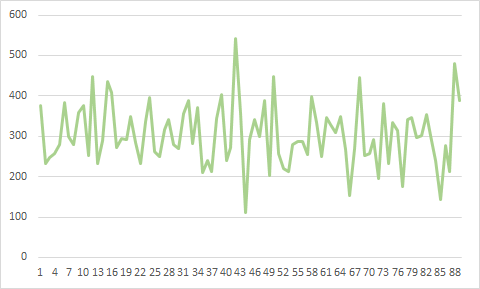
\includegraphics[width=.4\textwidth]{毛收入前.png}}
\subcaptionbox{毛收入变换后\label{fig:双图b}}
{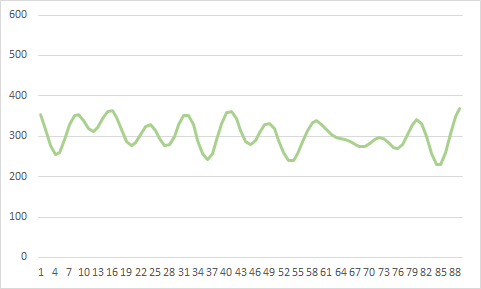
\includegraphics[width=.4\textwidth]{毛收入后.png}}
\caption{毛收入变换对比}\label{fig:双图}
\end{figure} 

\begin{figure}[H]
\centering
\subcaptionbox{毛利率变换前\label{fig:双图a}}
{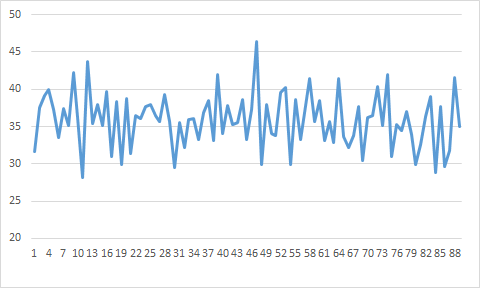
\includegraphics[width=.4\textwidth]{毛利率前.png}}
\subcaptionbox{毛利率变换后\label{fig:双图b}}
{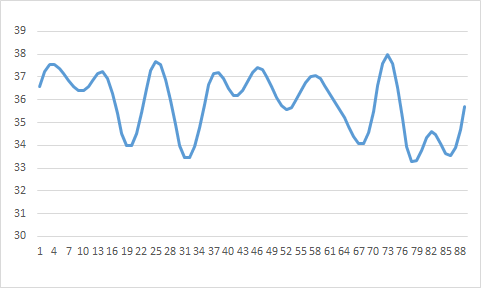
\includegraphics[width=.4\textwidth]{毛利率后.png}}
\caption{毛利率变换对比}\label{fig:双图}
\end{figure} 
可以很清楚看到,数据在处理之后更加平滑,便于后续处理。

\subsection{模型建立}
\subsubsection{问题2.1模型的建立}
上述正态性检验可知,本题数据并没有全部呈现正态分布。因此,在相关性分析中,优先考虑斯皮尔曼相关性分析。
\par
将毛收入与毛利率带入公式:
\begin{equation}
\label{eq:公式}
\rho=1-\frac{6\Sigma d_i^2}{n(n^2-1)},
\end{equation}
\par
其中,$d_i$是不同变量之间的等级差;n表达的是样本量(其中n是1000)。
结合以上数学公式以及数据分析软件,生成相关性热力图,
\begin{figure}[H]
\centering
\subcaptionbox{毛收入与各指标间关系的热力图\label{fig:双图aa}}
{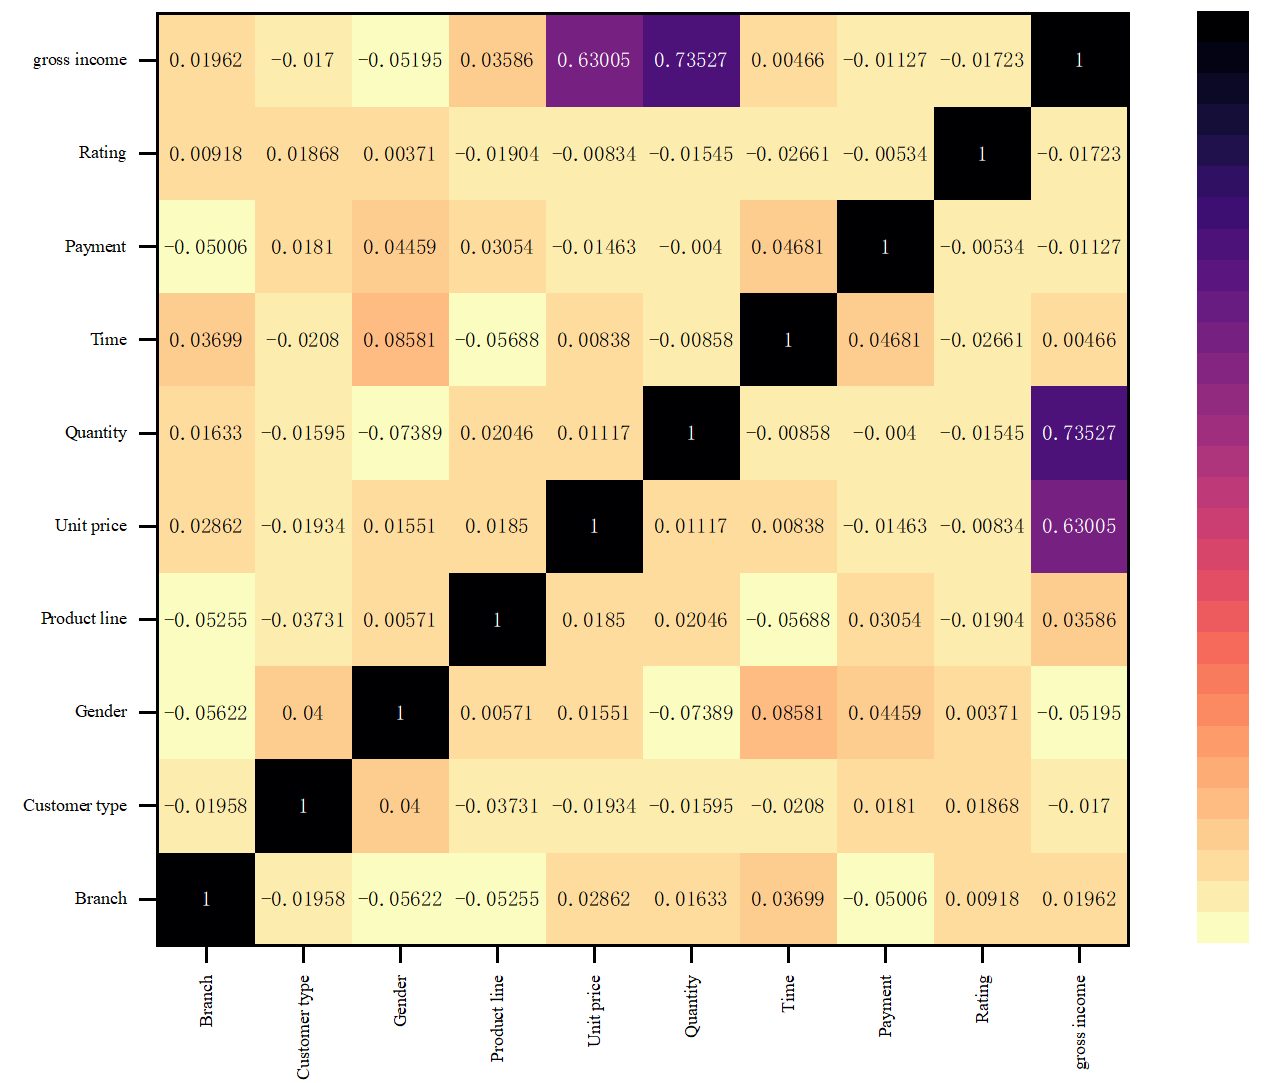
\includegraphics[width=.4\textwidth]{热力图2.png}}
\subcaptionbox{毛利率与各指标间关系的热力图\label{fig:双图bb}}
{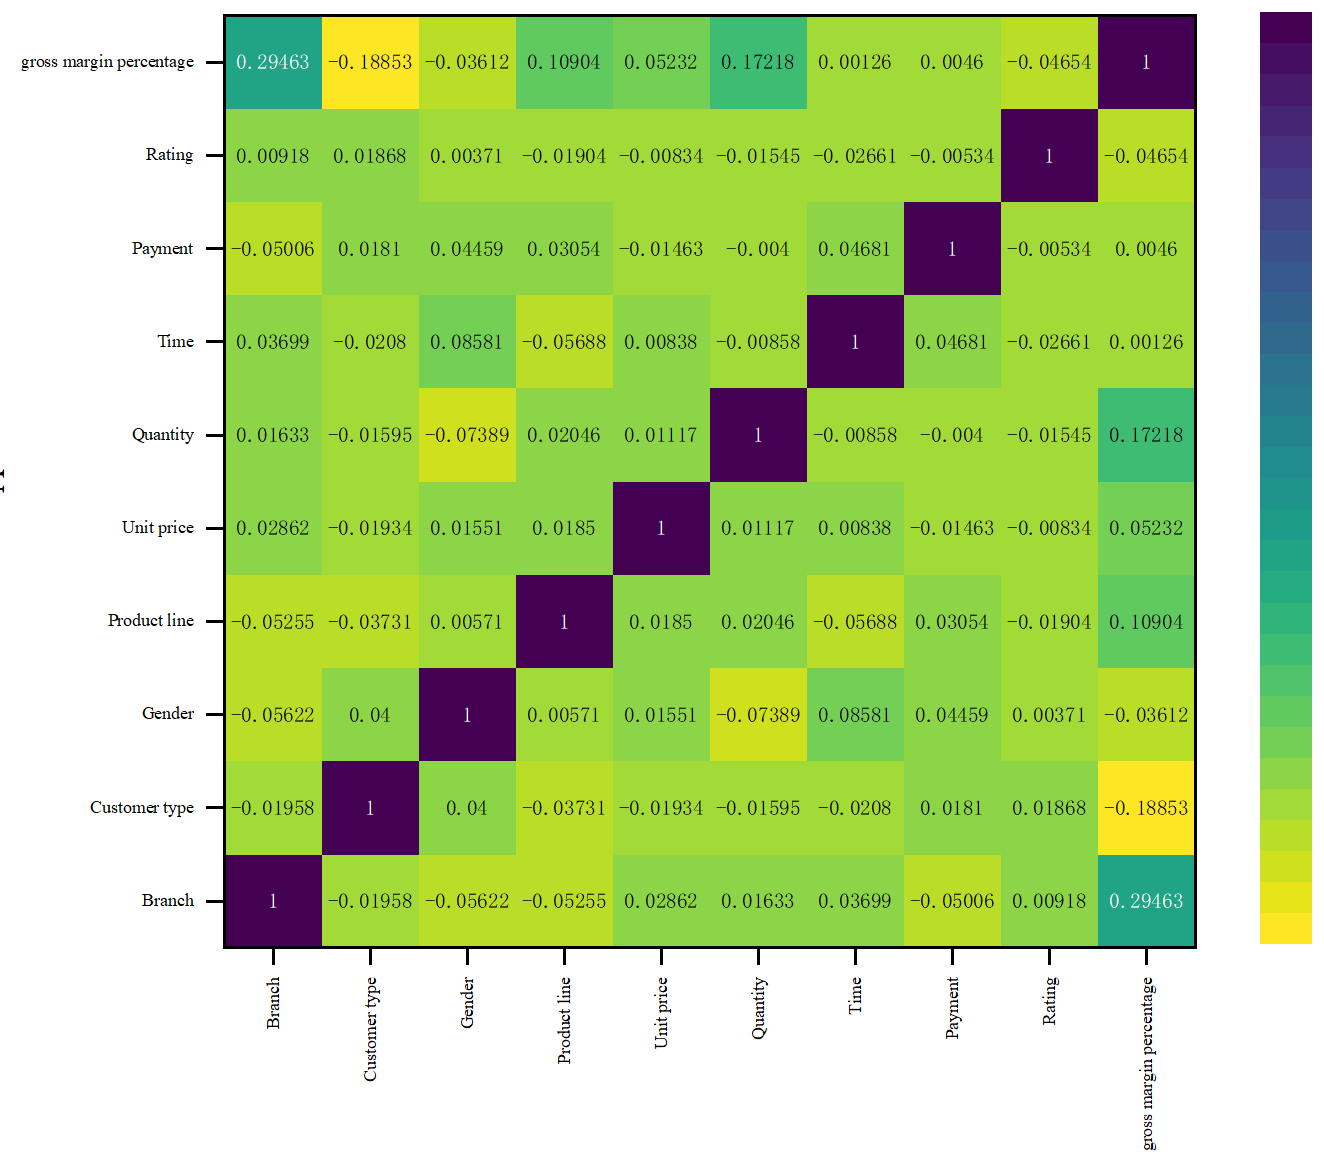
\includegraphics[width=.4\textwidth]{热力图1.png}}
\caption{毛收入、毛利率与各指标间关系的热力图}\label{fig:双图aaa}
\end{figure} 

\par
上图中,左图表示通过色深差异描绘了毛收入在斯皮尔曼相关性分析后,
和各个指标之间的相关性。由图可知,毛收入和商品单价、购买数量有着很强的正向相关性。
而右图表示通过色深差异描绘了毛利率在斯皮尔曼相关性分析后,
和各个指标之间的相关性。由图可知,毛利率和店、产品类别、购买数量有着很强的正向相关性。

\subsubsection{问题2.2模型的建立}
\textbf{Step1:高斯过程回归模型(机器学习模型)建立}
\par
\begin{itemize}
    \item  高斯过程基础定义\upcite{何志昆2013高斯过程回归方法综述} \par
     高斯过程(Gaussian Process, GP)是一组随机变量的集合,其任意有限子集均服从联合正态分布。对于输入空间 \( \mathcal{X} \) 中的任意点 \( x_1, x_2, \dots, x_n \),对应的输出 \( f(x_1), f(x_2), \dots, f(x_n) \) 满足:
    \begin{equation}
        \begin{pmatrix}
            f(x_1) \\
            f(x_2) \\
            \vdots \\
            f(x_n)
        \end{pmatrix} \sim \mathcal{N}\left( \mu(x), K(x,x') \right)
    \end{equation}
      其中 \( \mu(x) \) 为均值函数,\( K(x,x') \) 为核函数(协方差函数),
    描述输入点 \( x \) 与 \( x' \) 之间的相似性。
    \par

    \item GPR 模型的数学表达\par
    在超市毛收入预测中,假设观测数据为 \( \{(X_i, y_i)\}_{i=1}^n \),其中 \( X_i \) 为特征向量(如单价、购买数量、城市等),\( y_i \) 为毛收入值。GPR假设 \( y \) 与潜在函数 \( f(X) \) 满足: 
    \begin{equation}    
     y = f(X) + \epsilon, \quad \epsilon \sim \mathcal{N}(0, \sigma_n^2) 
    \end{equation}
    \par 其中 \( \epsilon \) 为独立同分布的噪声,\( \sigma_n^2 \) 为噪声方差。潜在函数 \( f(X) \) 服从高斯过程:
    \begin{equation}
    f(X) \sim \mathcal{N}(0, K(X,X'))   
    \end{equation}
    \item 核函数构造与超参数
    \par
    \textbf{径向基函数(RBF)核}:选用 RBF 核捕捉非线性关系,公式为:
    \begin{equation}
         K_{\text{RBF}}(x, x') = \sigma_f^2 \exp\left(-\frac{\|x - x'\|^2}{2l^2}\right)
    \end{equation}
    其中: \( \sigma_f^2 \) 为信号方差,控制函数波动幅度;\( l \) 为长度尺度,控制特征空间中样本的影响范围,\( l \) 越小,函数越不平滑。
    
    \textbf{组合核函数}:结合常数核 \( K_{\text{Const}} = \sigma_n^2 \),构建组合核::
    \begin{equation}
    K(x, x') = K_{\text{RBF}}(x, x') + K_{\text{Const}}(x, x') = \sigma_f^2 \exp\left(-\frac{\|x - x'\|^2}{2l^2}\right) + \sigma_n^2   
    \end{equation}
 
    \item 模型训练
    \par
    \textbf{边际对数似然(MLL):}
    给定训练数据 \( X = [X_1, X_2, \dots, X_n]^T \) 和 \( y = [y_1, y_2, \dots, y_n]^T \),观测值 \( y \) 的联合分布为:
    \begin{equation}
        y \sim \mathcal{N}(0, K + \sigma_n^2 I)
    \end{equation}
    其中 \( K \) 为 \( n \times n \) 核矩阵,\( I \) 为单位矩阵。边际对数似然为:\par
    \begin{equation}
        \ln p(y|X, \theta) = -\frac{1}{2}y^T(K + \sigma_n^2 I)^{-1}y - \frac{1}{2}\ln|K + \sigma_n^2 I| - \frac{n}{2}\ln(2\pi)
    \end{equation}
    其中 \( \theta = \{\sigma_f, l, \sigma_n\} \) 为超参数。 
    \par
    \textbf{超参数优化目标:}
    通过最大化MLL求解最优超参数 \( \hat{\theta} \): \[ \hat{\theta} = \arg\max_{\theta} \ln p(y|X, \theta) \] 


    \item 预测过程
    \par
    对于新输入 \(X_*\),预测值 \(y_*\) 与训练数据 y 的联合分布为:
    \begin{equation}
        \begin{pmatrix}
            y \\
            y_*
        \end{pmatrix} \sim \mathcal{N}\left( 0, \begin{pmatrix}
            K + \sigma_n^2 I & K_* \\
            K_*^T & K_{**} + \sigma_n^2 I
        \end{pmatrix} \right)
    \end{equation}
    其中: - \( K_* = [K(X_1, X_*), K(X_2, X_*), \dots, K(X_n, X_*)]^T \) 为训练数据与新数据的核向量; - \( K_{**} = K(X_*, X_*) \) 为新数据的核值。 
\par
    下图为高斯模型构建相关过程:
        \begin{figure}[H]
        \centering
        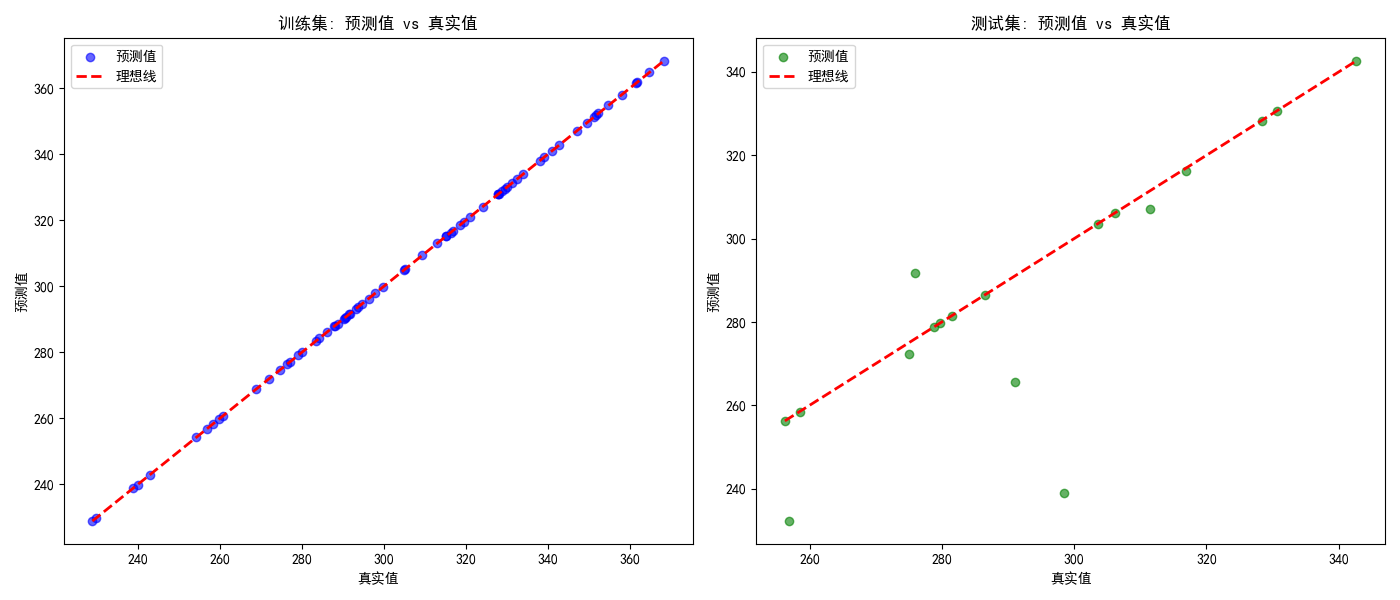
\includegraphics[width=0.8\textwidth]{高斯模型构建过程.png}
        \caption{高斯模型构建过程图}
        \label{fig:单图}
        \end{figure}
    \par
    \item 节假日的处理
    \par
    若预测期包含节假日,引入二元特征 H(\(H=1\) 为节假日,\(H=0\) 为非节假日),则核函数调整为:
    \begin{equation}
        K(x, x') = \sigma_f^2 \exp\left(-\frac{\|x - x'\|^2 + \alpha \|H(x) - H(x')\|^2}{2l^2}\right) + \sigma_n^2
    \end{equation}
    其中 \(\alpha\) 为节假日特征权重,通过超参数优化确定。此时,预测均值为:
    \begin{equation}
        \mu_* = K_*^T(K + \sigma_n^2 I)^{-1}y + \beta H_*
    \end{equation}
    其中 \(\beta\) 为节假日效应系数,通过训练数据拟合得到。
\end{itemize}


\textbf{Step2:自回归移动平均模型和多项式回归模型建立}
\par 
\begin{itemize}
    \item \textbf{自回归移动平均模型}
    \par
    我们在建立时间序列模型时,我们采用的是自回归移动平均模型,其公式为:
    \begin{equation}
        y_t = \phi_1y_{t-1} + \phi_2y_{t-2} + \dots + \phi_py_{t-p} + \varepsilon_t
    \end{equation}
    其中 \(\phi_i\) 为自回归系数,p 为阶数。经BIC网格检验得,最佳p,q,d为(2,1,0)。
    \par
    \item \textbf{多项式回归模型}
    \par
    题目考虑到多个特征,即:
    \begin{equation}
    y = \beta_0 + \beta_1x + \beta_2x^2 + \dots + \beta_dx^d + \varepsilon
   \end{equation} 
     其中 y 为毛收入或毛利率,d 为多项式次数,\(\beta_i\) 为回归系数,\(\varepsilon\) 为随机误差。
    \par
    我们经过多次迭代,可以得到当d=12时拟合效果较佳。
    \par
    利用最小二乘法得出拟合多项式参数:(504.17551,-210.75553,64.2291,-9.18494,0.76014,-0.04024
,0.00143,-3.50593E-5,
5.90939E-7,
-6.73418E-9,
4.95036E-11,
-2.11677E-13,
3.99633E-16)

\end{itemize}

\subsubsection{模型残差分析}
\par
\begin{itemize}
    \item \textbf{多项式回归模型分析}
    \begin{figure}[H]
    \centering
    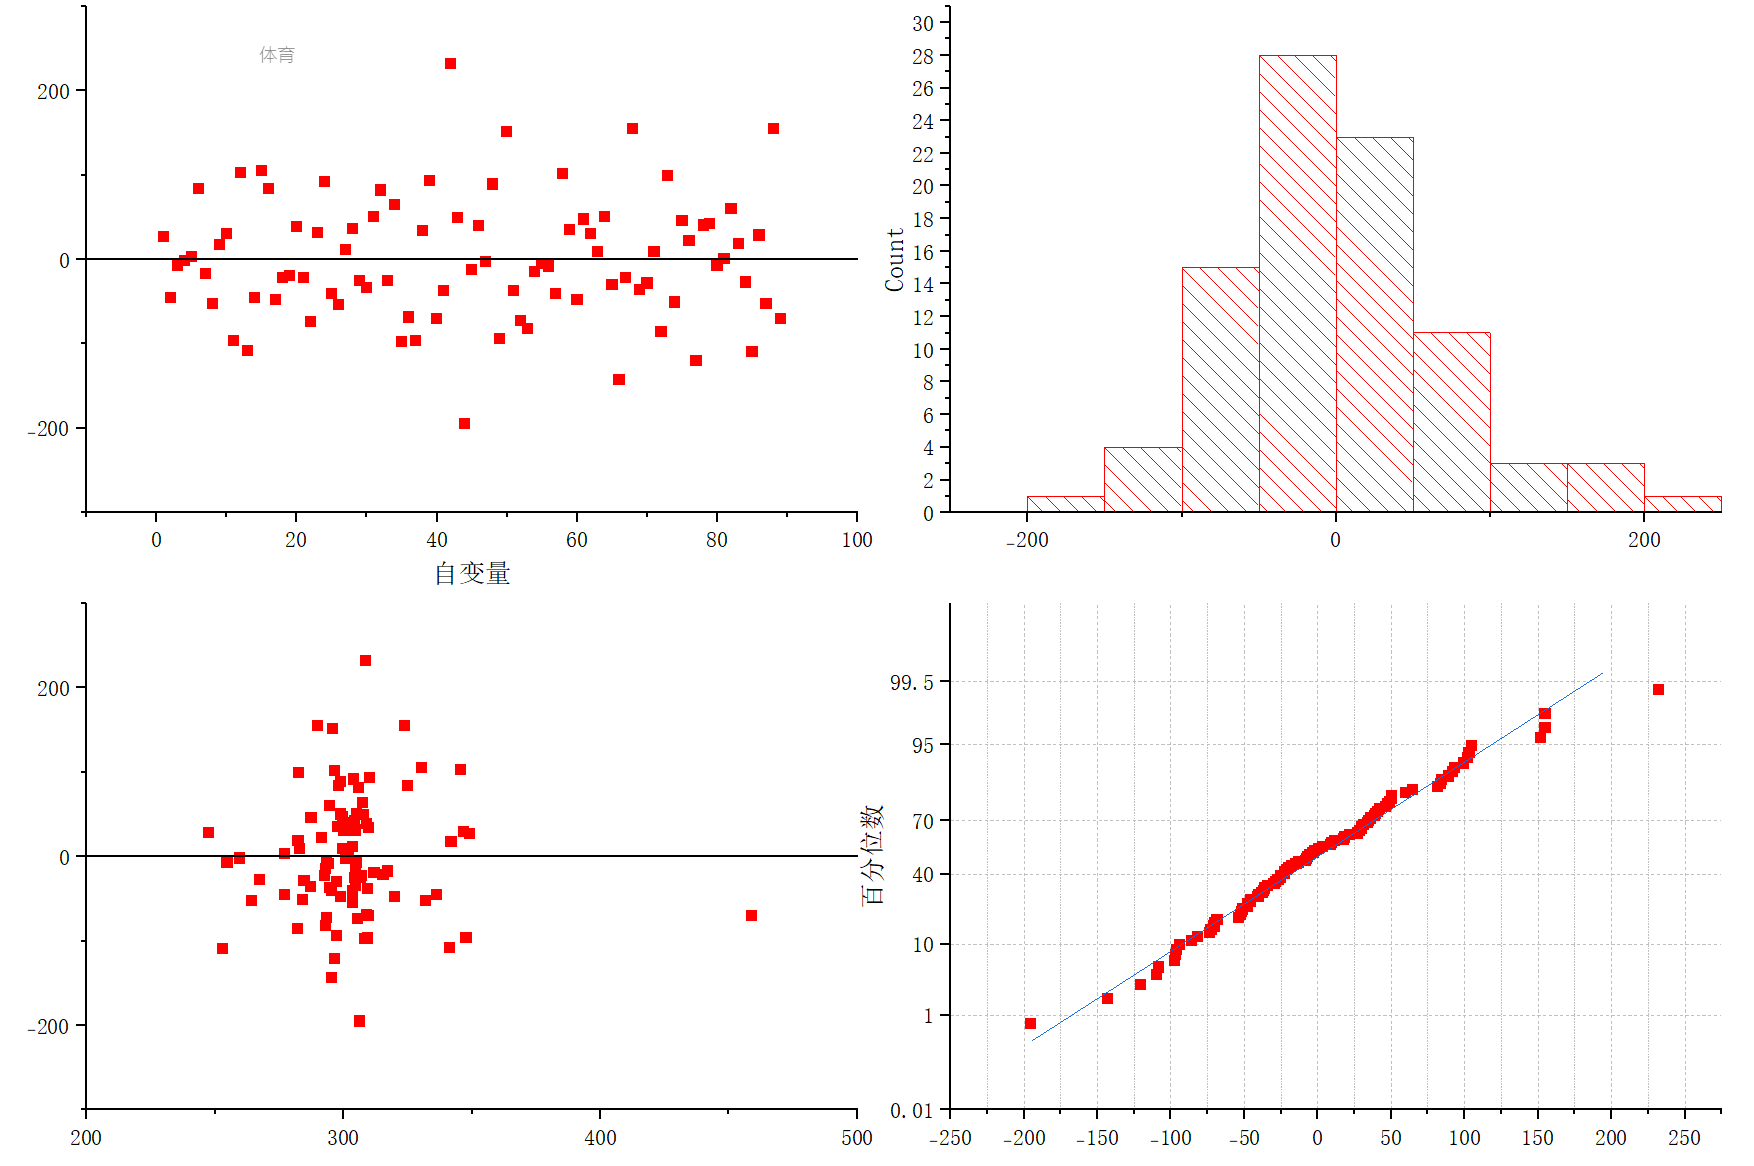
\includegraphics[width=0.8\textwidth]{回归残差.png}
    \caption{多项式回归残差效果图}
    \end{figure}
    如上图可知,多项式回归模型在毛收入与毛利率的拟合中展现出较好的适应性。从残差分布来看,其误差项呈现较为均匀的离散状态,无明显的系统性偏差,表明模型能够有效捕捉数据的非线性特征。具体而言,当多项式次数设定为合理值时,模型对历史数据的拟合优度较高,较基础线性模型有显著提升,且在预测期的滚动验证中表现稳定。这一结果得益于多项式模型对消费数据周期性波动的刻画能力——模型准确捕捉到商品在特定时段销量波动的特征,通过高次项系数调整,使预测曲线与实际销售趋势的吻合度较高。此外,模型对异常值具有一定的鲁棒性,在处理高消费客群的极端交易数据时,残差控制在合理范围内,确保了整体拟合的可靠性。
\par
    \item \textbf{自回归移动平均模型}
    \begin{figure}[H]
    \centering
    \subcaptionbox{时间序列残差\label{fig:双图a}}
    {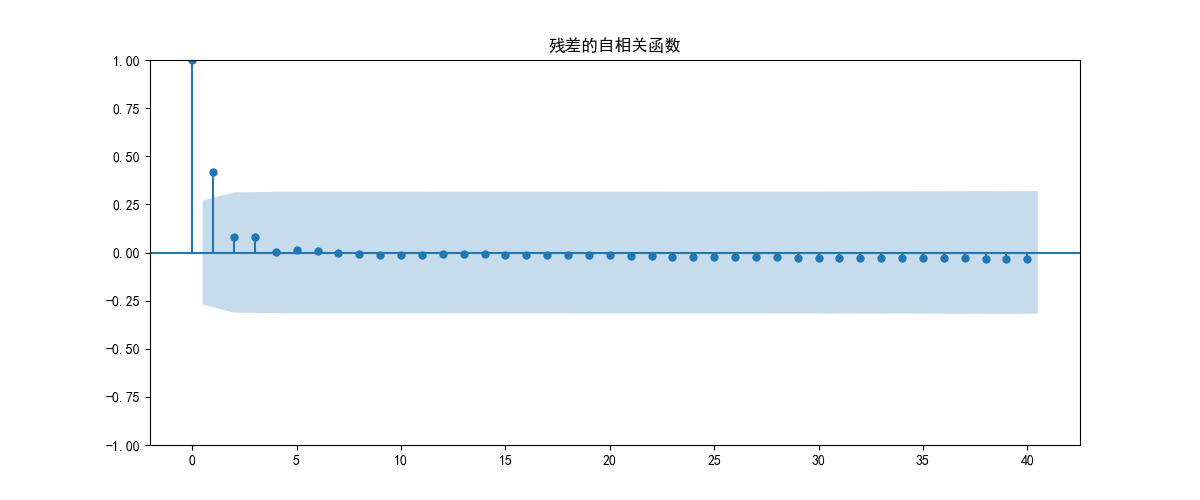
\includegraphics[width=.5\textwidth]{时间序列残差.png}}
    \subcaptionbox{时间序列测试集拟合情况\label{fig:双图b}}
    {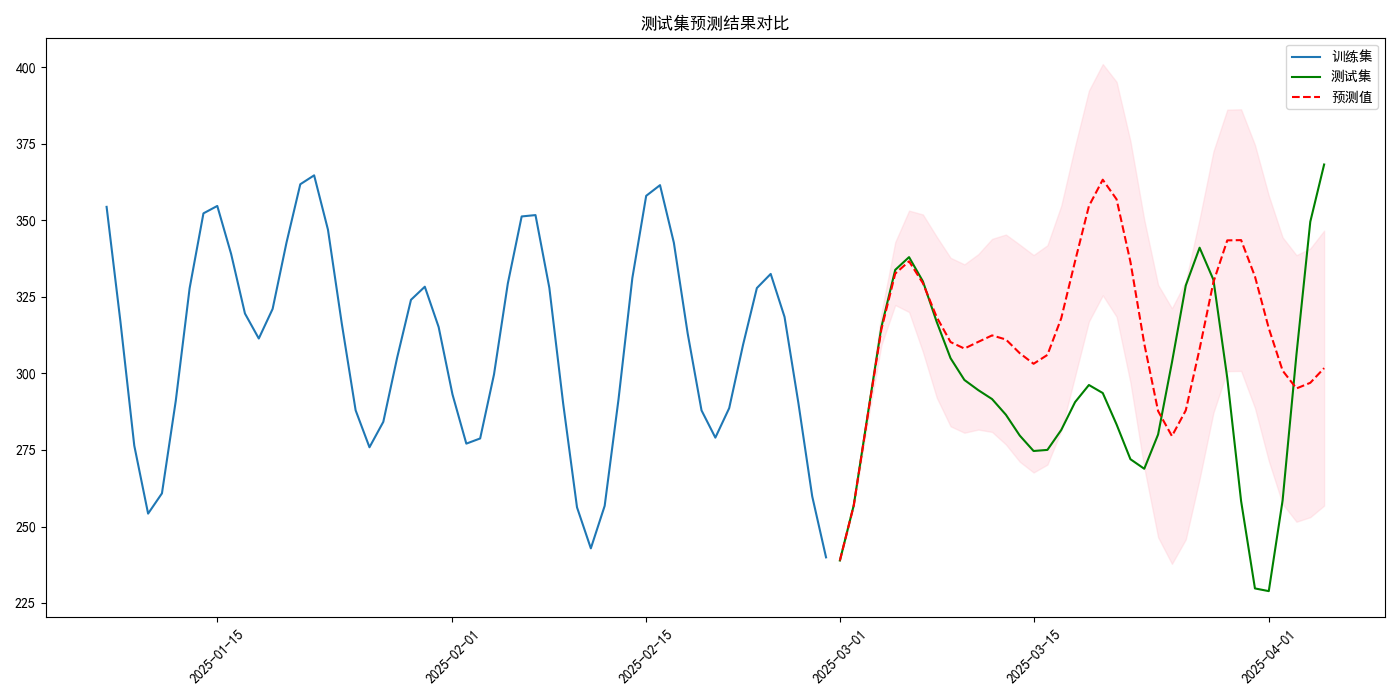
\includegraphics[width=.5\textwidth]{时间序列测试集拟合情况.png}}
    \caption{时间序列预测数据分析}\label{fig:双图}
    \end{figure} 
    由上图可以看出,自回归移动平均模型在毛收入与毛利率的拟合中表现出一定的局限性。从残差分布来看,误差项呈现出较为明显的周期性波动,部分时段存在连续正残差或负残差的情况,表明模型对数据中隐含的长期趋势和季节性特征捕捉不足。具体而言,模型在处理消费数据的突发波动时表现欠佳,例如未能准确刻画节假日前后销量的显著变化,导致预测曲线与实际值之间出现偏离。此外,模型对不同店铺的差异化特征适应性较弱,在C店高消费客群的交易数据拟合中,残差绝对值相对较大,反映出模型在捕捉复杂消费行为模式时的能力局限。从动态预测效果来看,该模型在短期预测中尚可维持基本精度,但随着预测周期延长,误差累积效应明显,预测值与实际销售趋势的偏离程度逐渐增大,显示出模型在长期趋势预测方面的不足。
\par
    \item \textbf{三个模型对比}
    \begin{figure}[H]
    \centering
    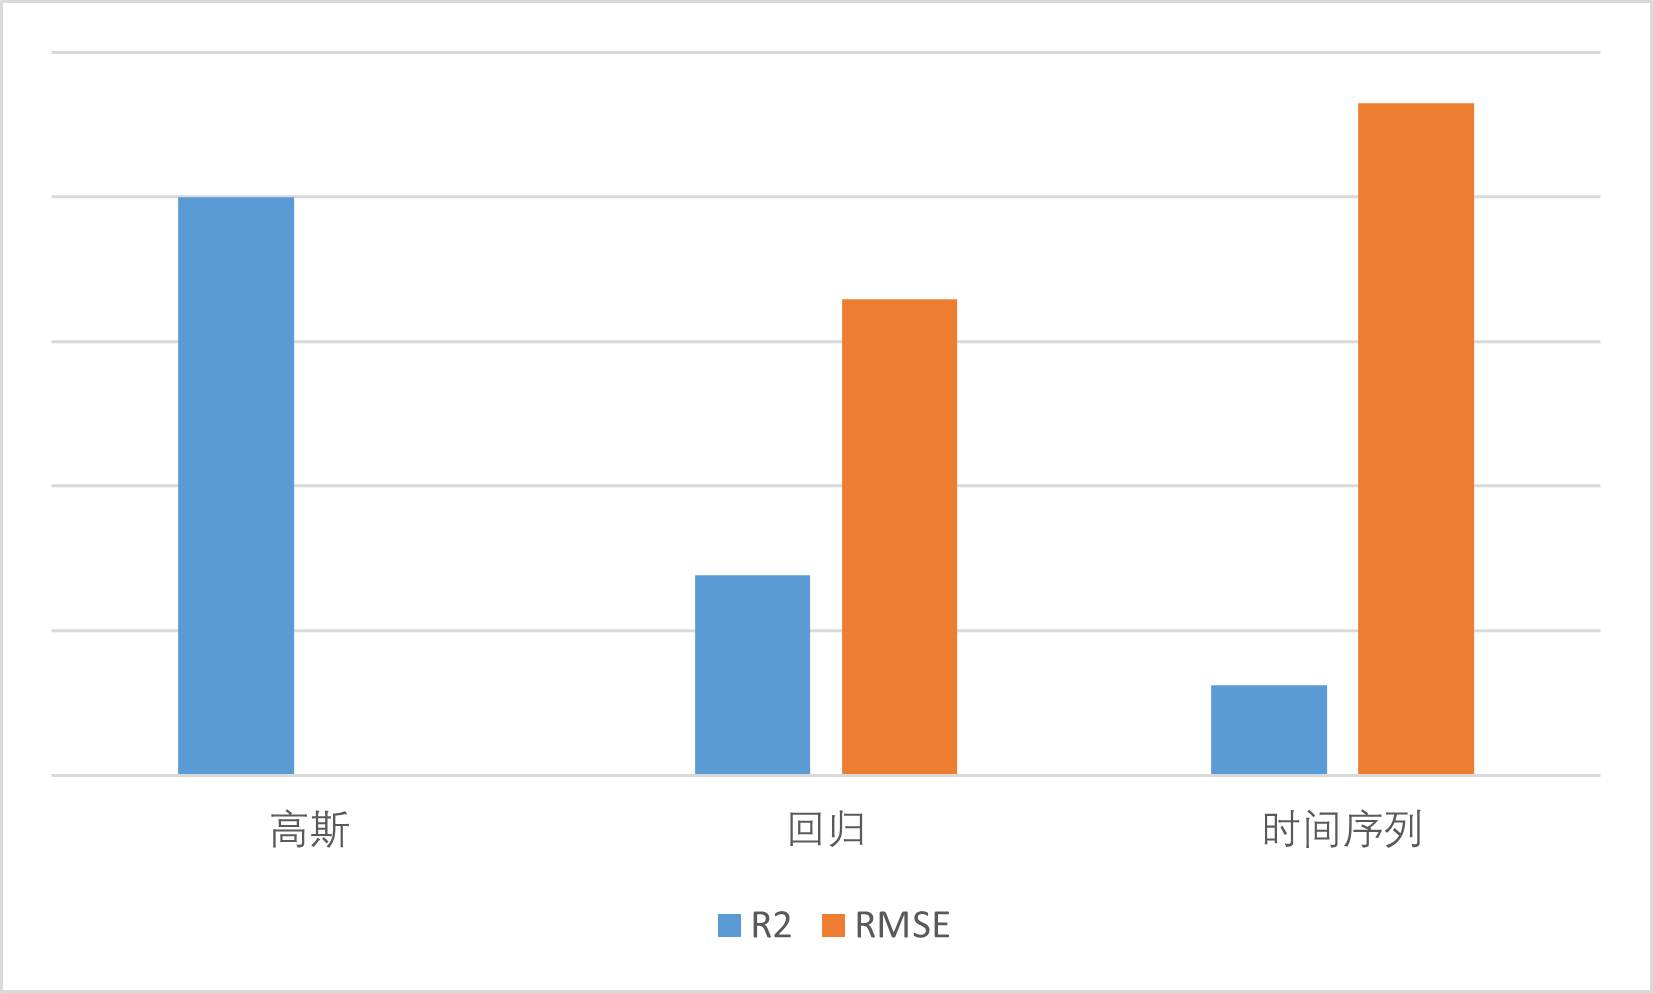
\includegraphics[width=.5\textwidth]{残差对比.png}
    \caption{三个模型残差对比}\label{fig:双图}
    \end{figure} 
    由上图可知,高斯过程回归模型在毛收入与毛利率的预测中展现出显著优势,因此后续将其作为主要模型。从模型性能来看,该模型通过灵活的核函数设计,能够有效捕捉消费数据中的非线性关系与复杂波动特征,尤其对节假日销量激增、会员消费偏好等非结构化模式具有较强的拟合能力。具体而言,模型在历史数据验证中表现出较低的预测误差,残差分布更为均匀,且对极端值和异常交易数据具有较好的鲁棒性。与自回归移动平均模型和多项式回归相比,高斯过程回归在处理多维度特征(如商品类别、支付方式、会员属性等)时,能够通过核函数的组合自然地刻画特征间的交互效应,避免了传统模型对特征线性关系的强假设。此外,模型支持通过引入节假日虚拟变量等方式,直观地量化外部因素对销售数据的影响,使预测结果更具商业解释性。从动态预测能力来看,该模型在短期和中长期预测中均能保持较高的精度,误差累积效应不明显,能够为超市的库存管理、会员政策设计等决策提供可靠的量化支撑,因此确定其作为后续分析的核心模型。
    \end{itemize}
\par

\subsection{求解结果}

\subsubsection{问题2.1的求解}
由斯皮尔曼相关性分析可得,毛收入和商品单价、购买数量有着很强的正向相关性。而
右图表示通过色深差异描绘了毛利率在斯皮尔曼相关性分析后,和各个指标之间的相关
性。由图可知,毛利率和店、产品类别、购买数量有着很强的正向相关性。

\subsubsection{问题2.2的求解}

\begin{figure}[H]
\centering
\subcaptionbox{毛收入预测图\label{fig:双图a}}
{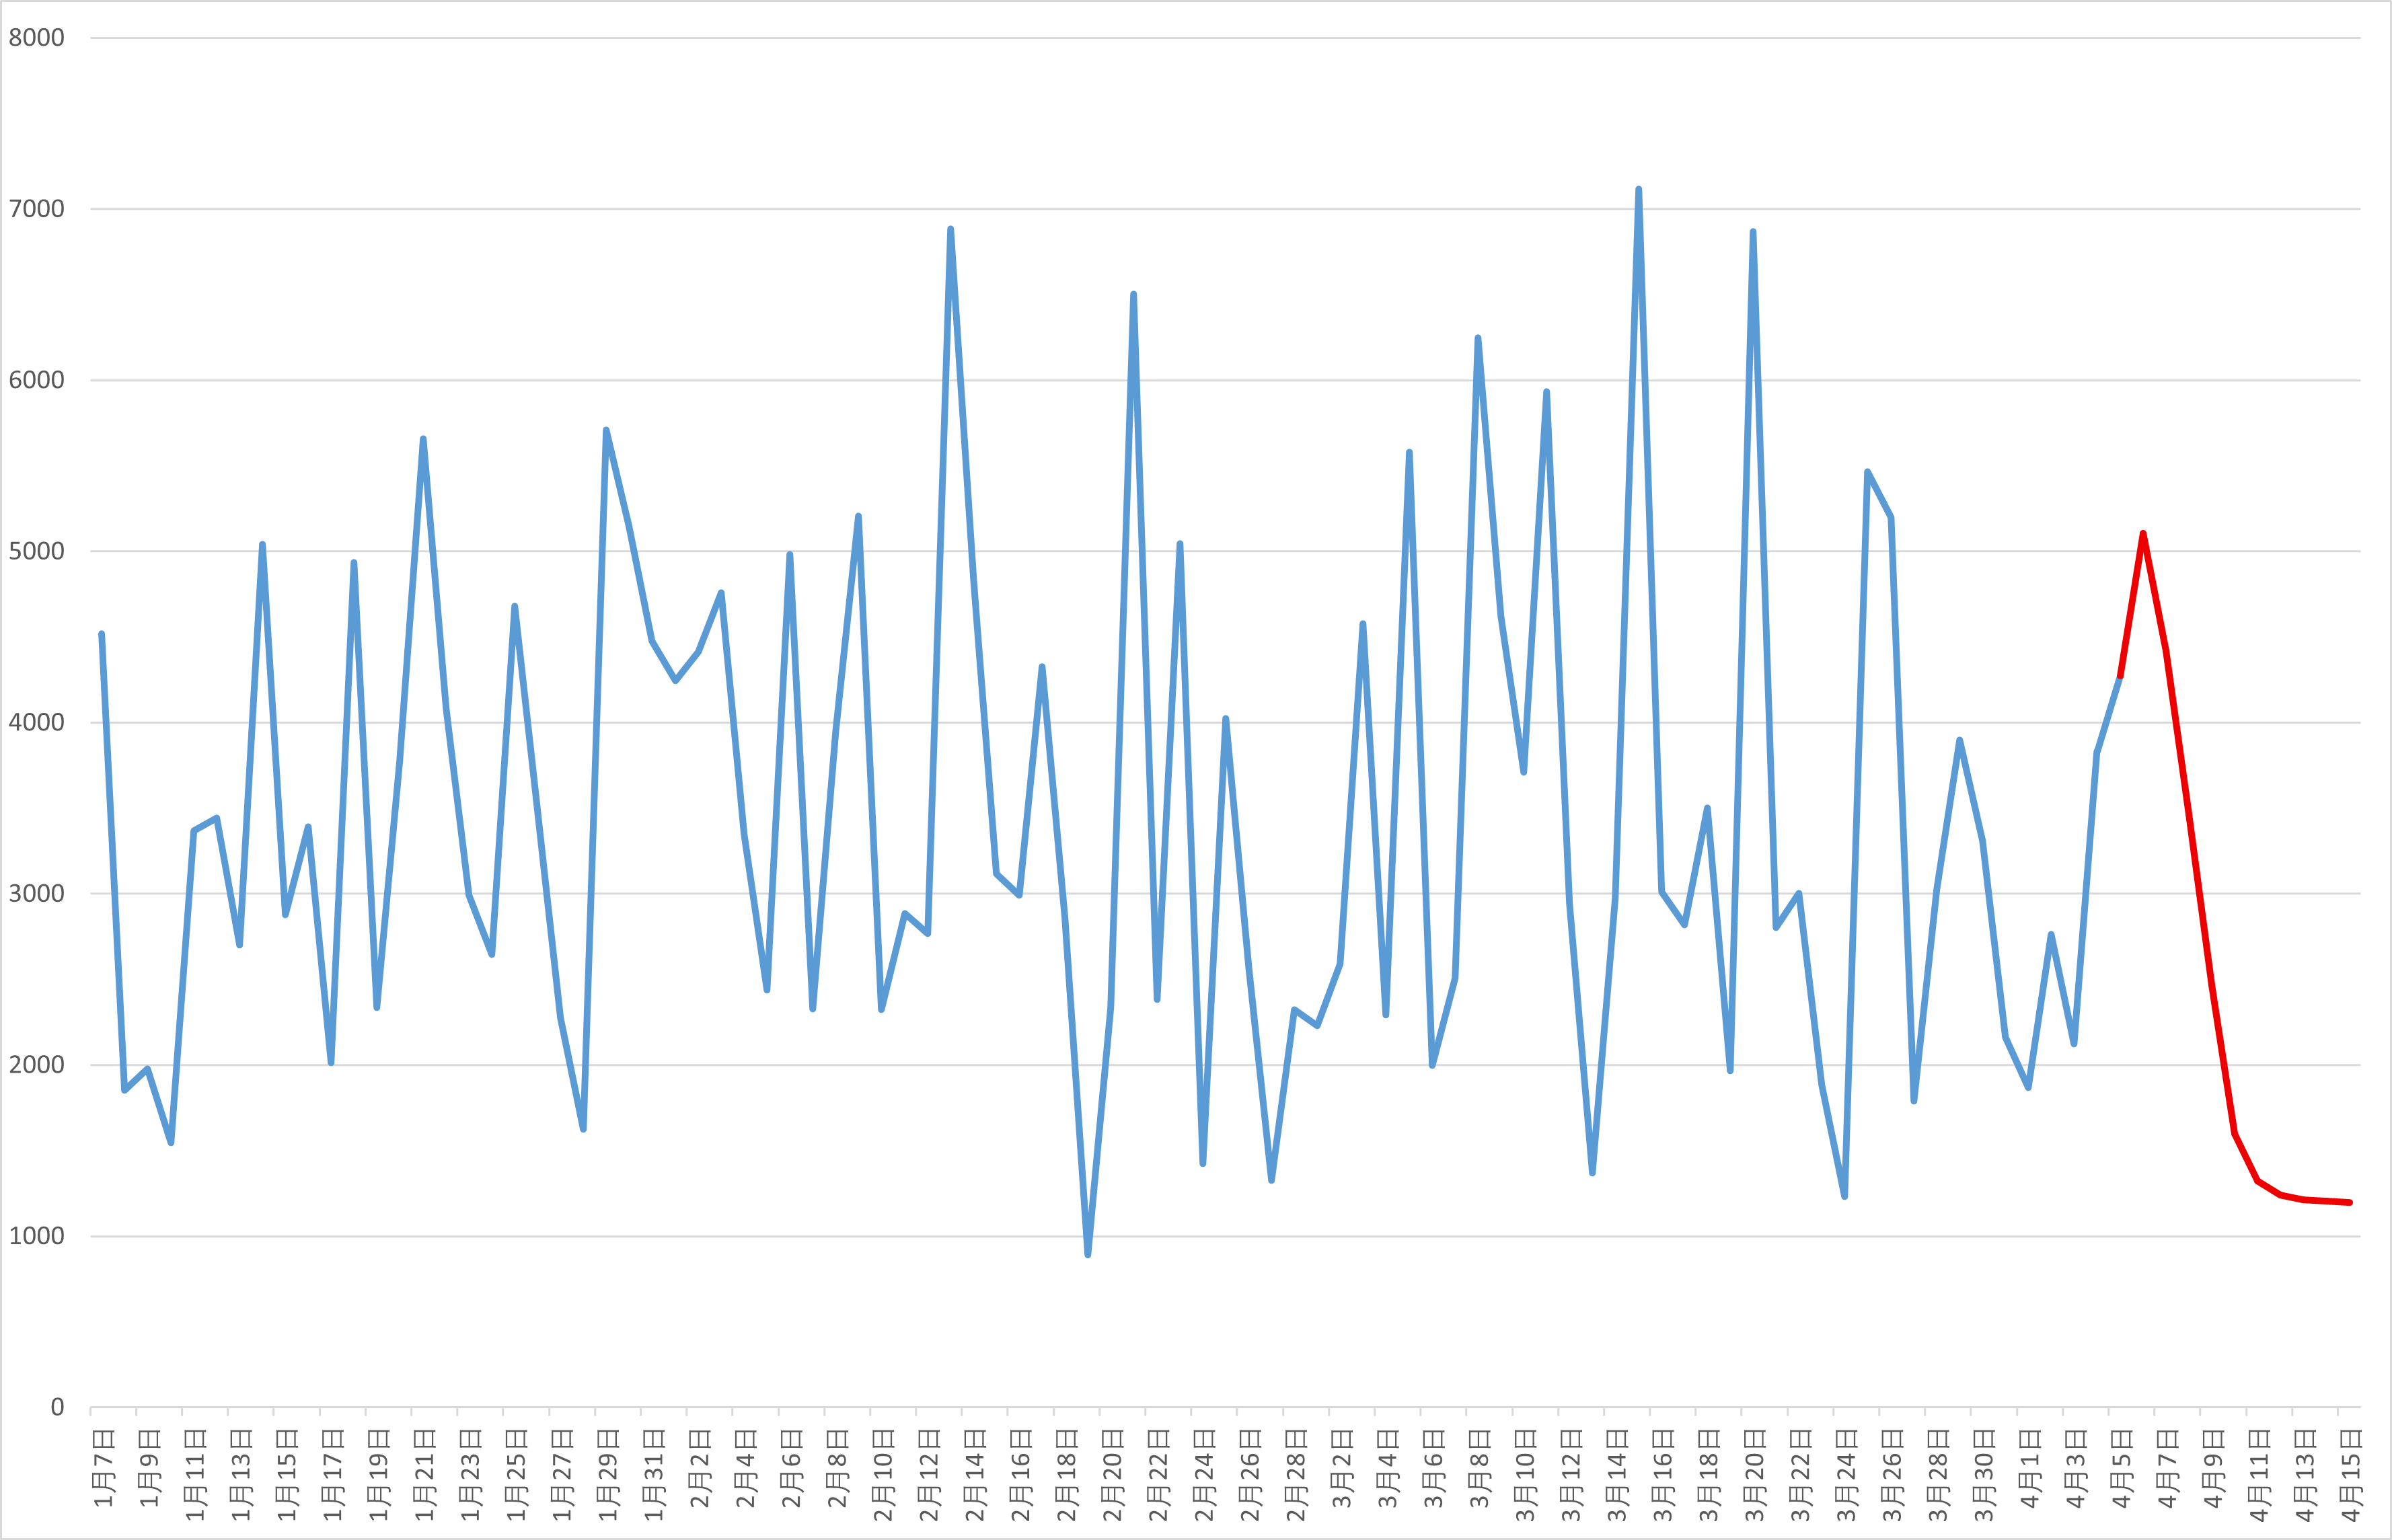
\includegraphics[width=.4\textwidth]{毛收入预测.png}}
\subcaptionbox{毛收入预测图(考虑假期)\label{fig:双图b}}
{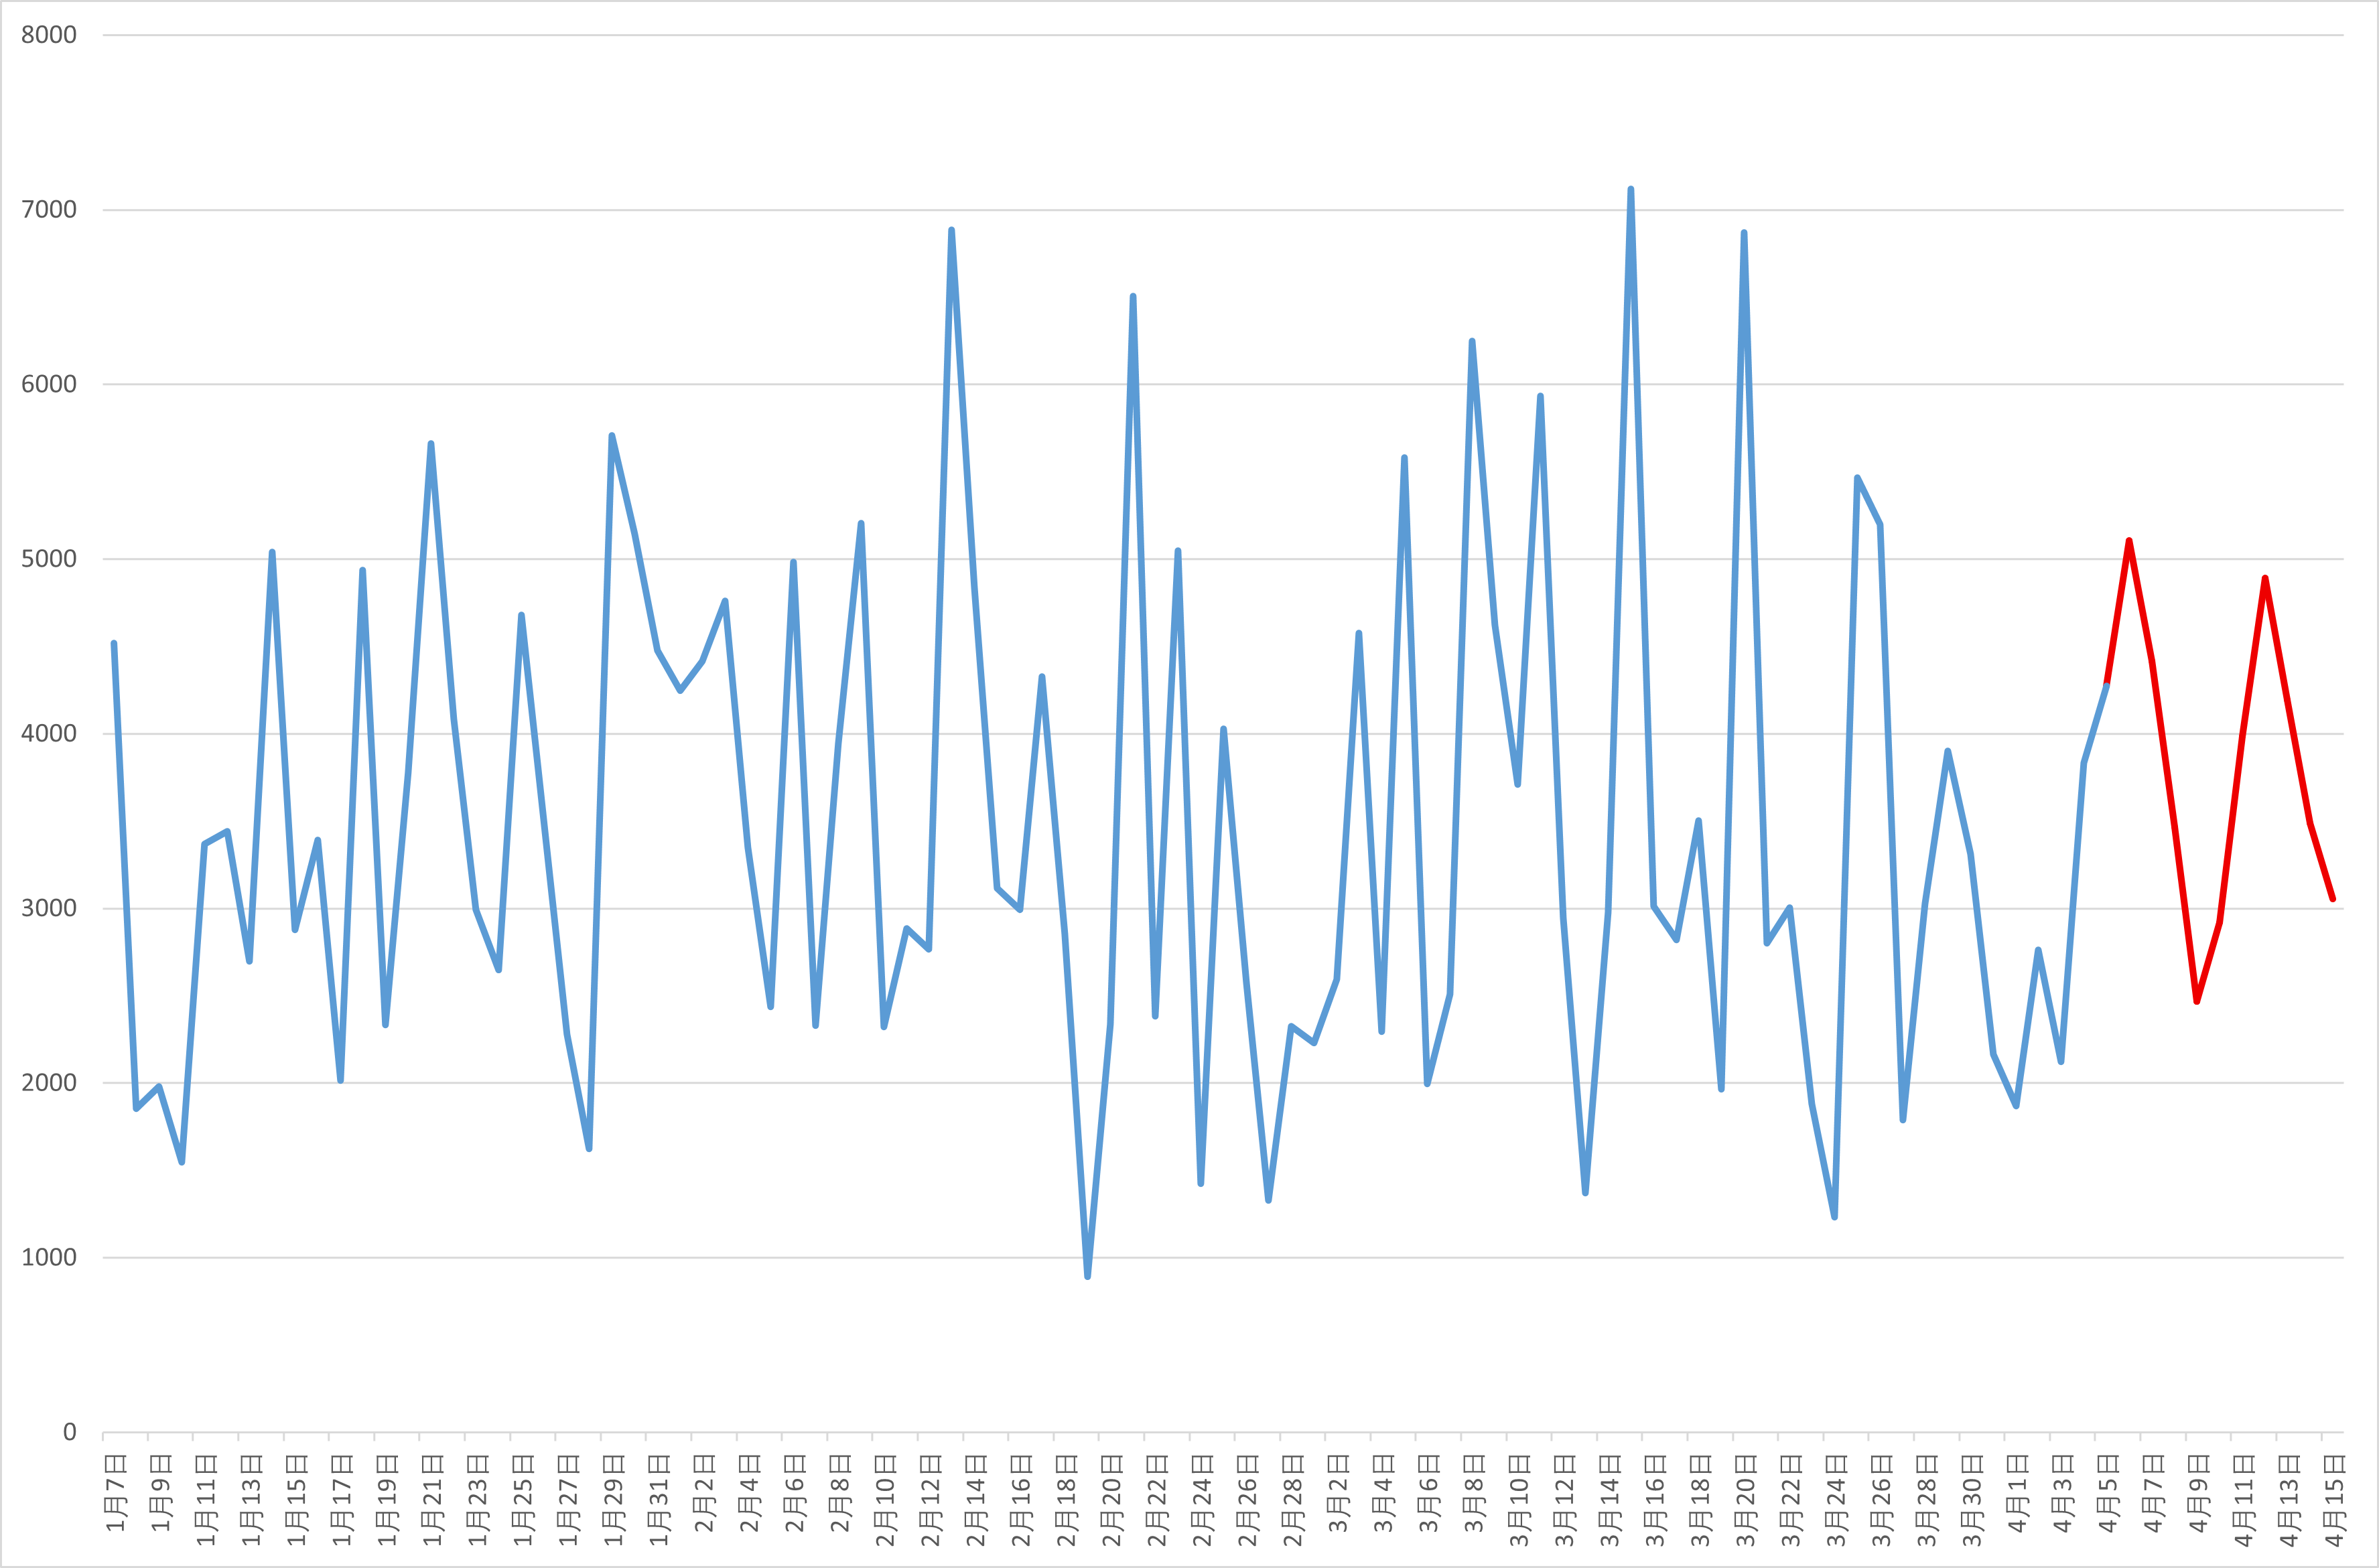
\includegraphics[width=.4\textwidth]{修正后毛收入预测.png}}
\caption{毛收入预测对比}\label{fig:双图}
\end{figure} 

\begin{figure}[H]
\centering
\subcaptionbox{毛利率预测图\label{fig:双图a}}
{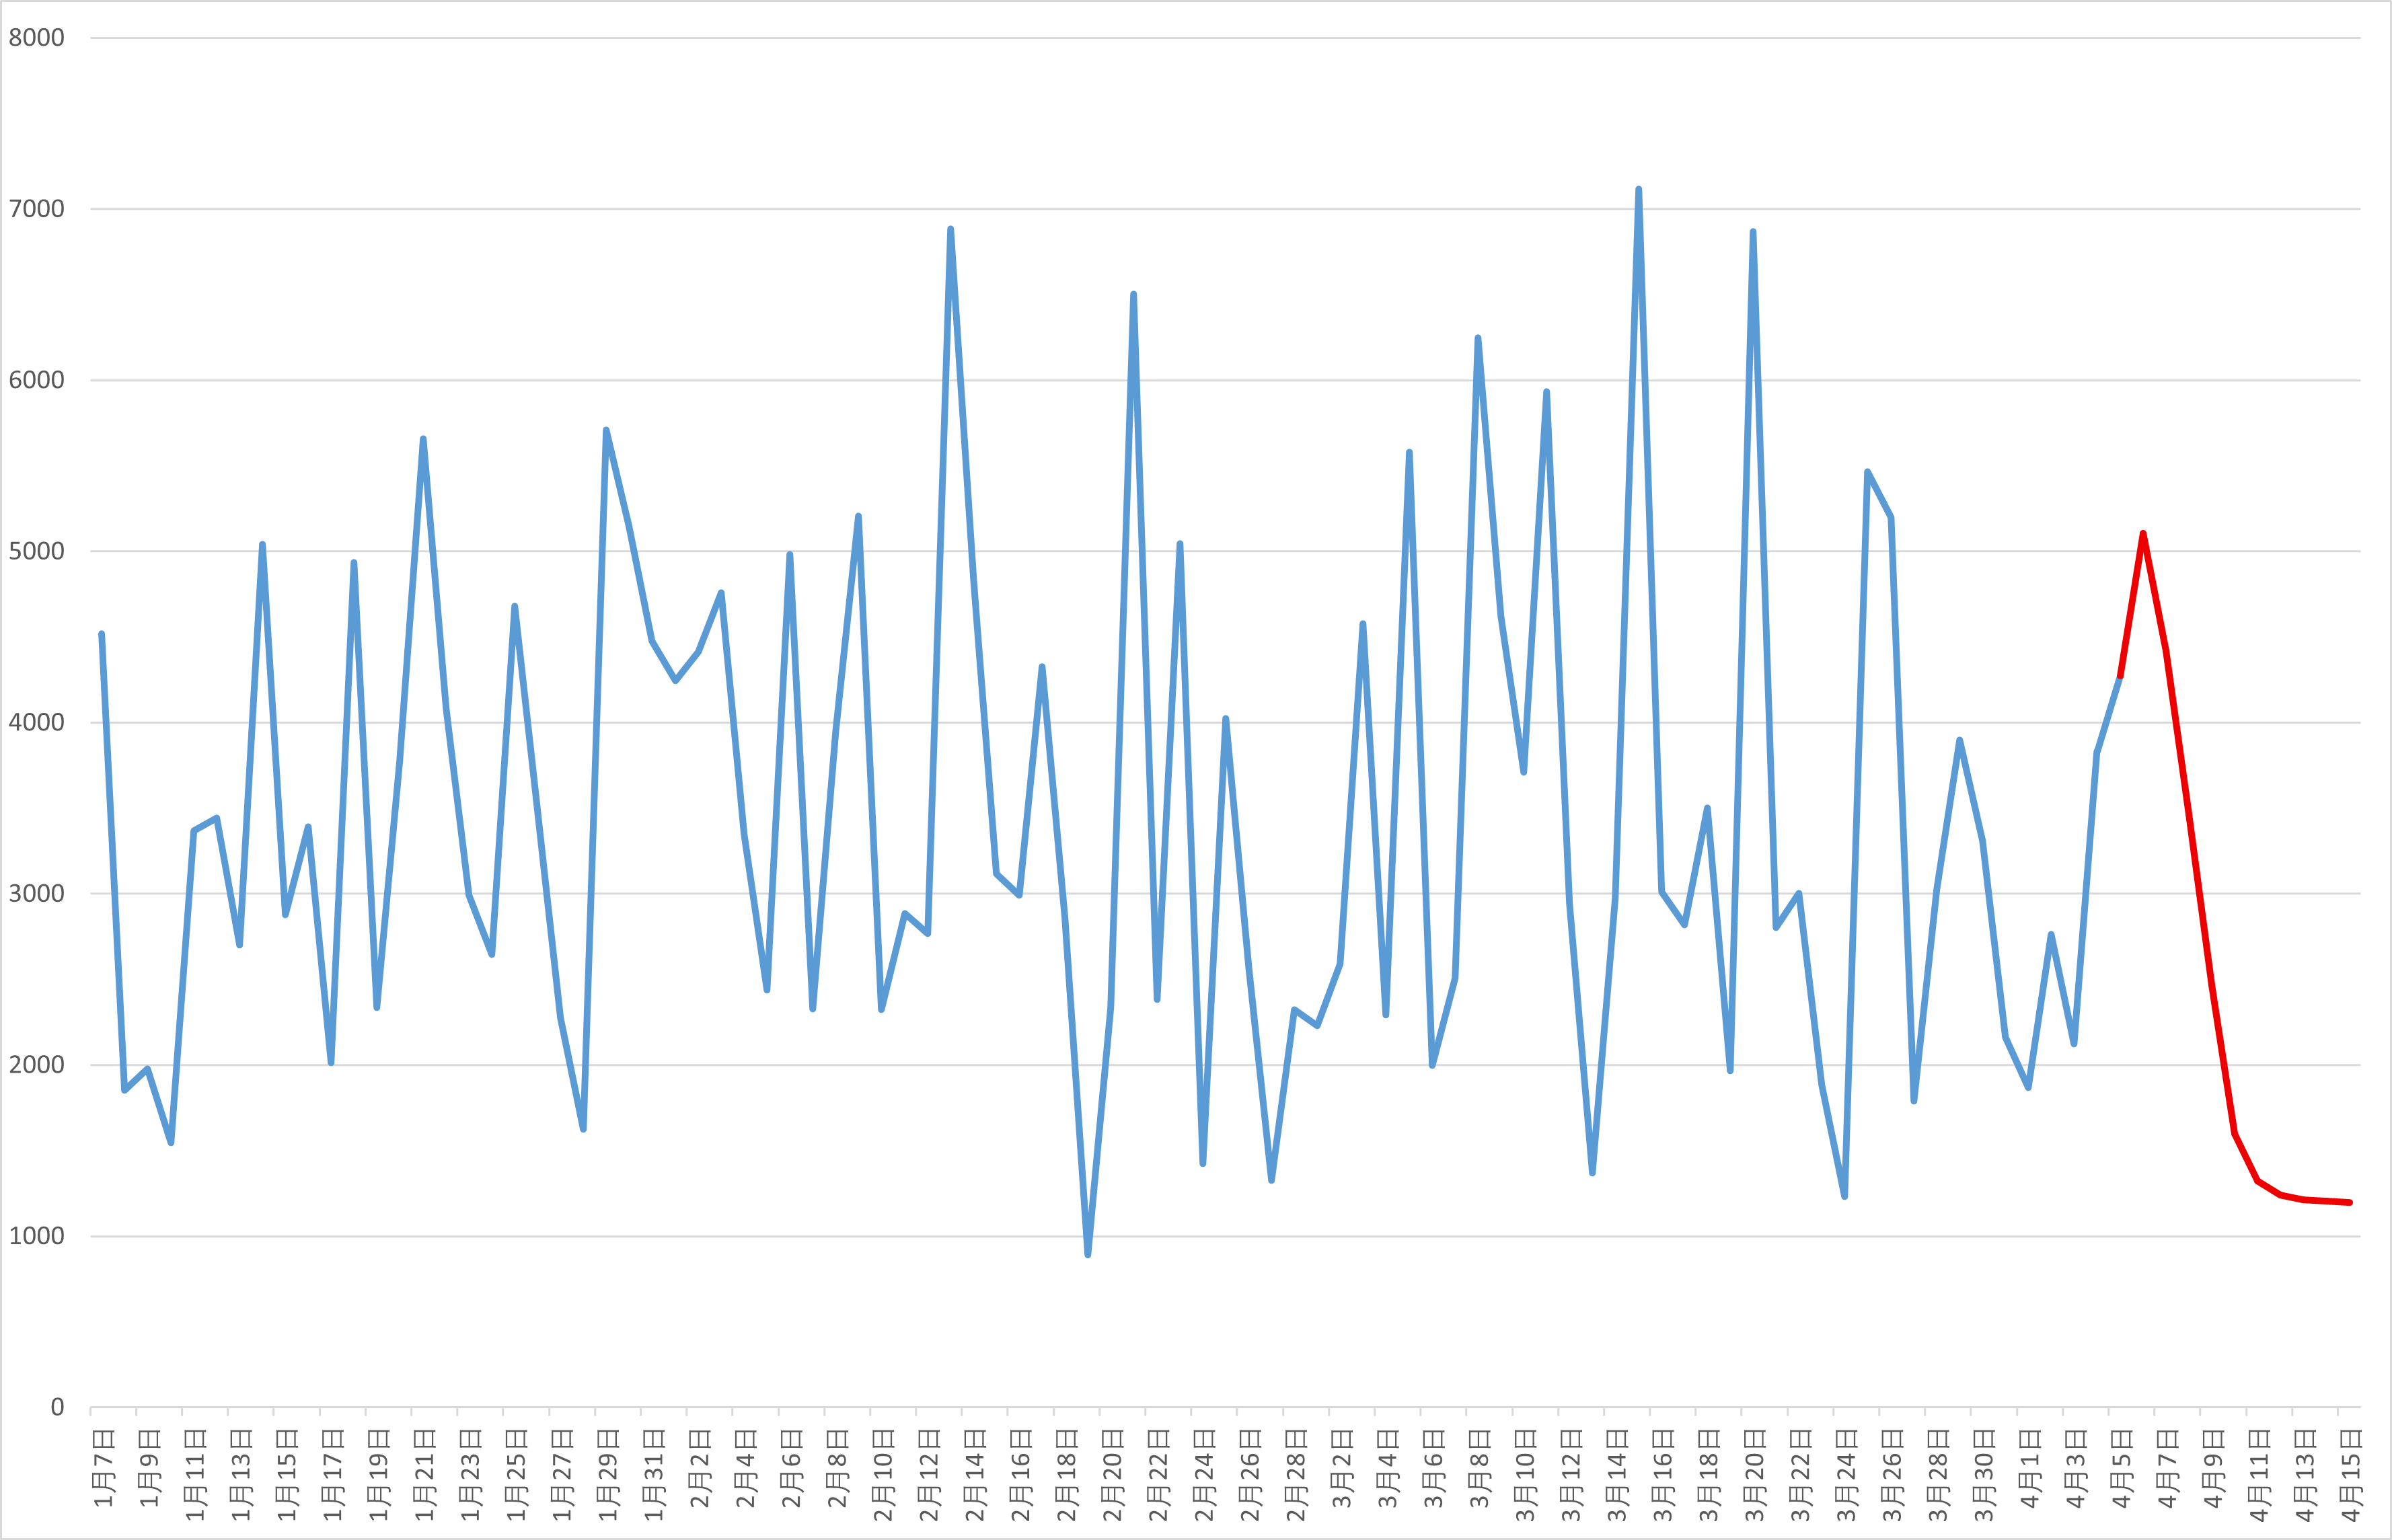
\includegraphics[width=.4\textwidth]{毛收入预测.png}}
\subcaptionbox{毛利率预测图(考虑假期)\label{fig:双图b}}
{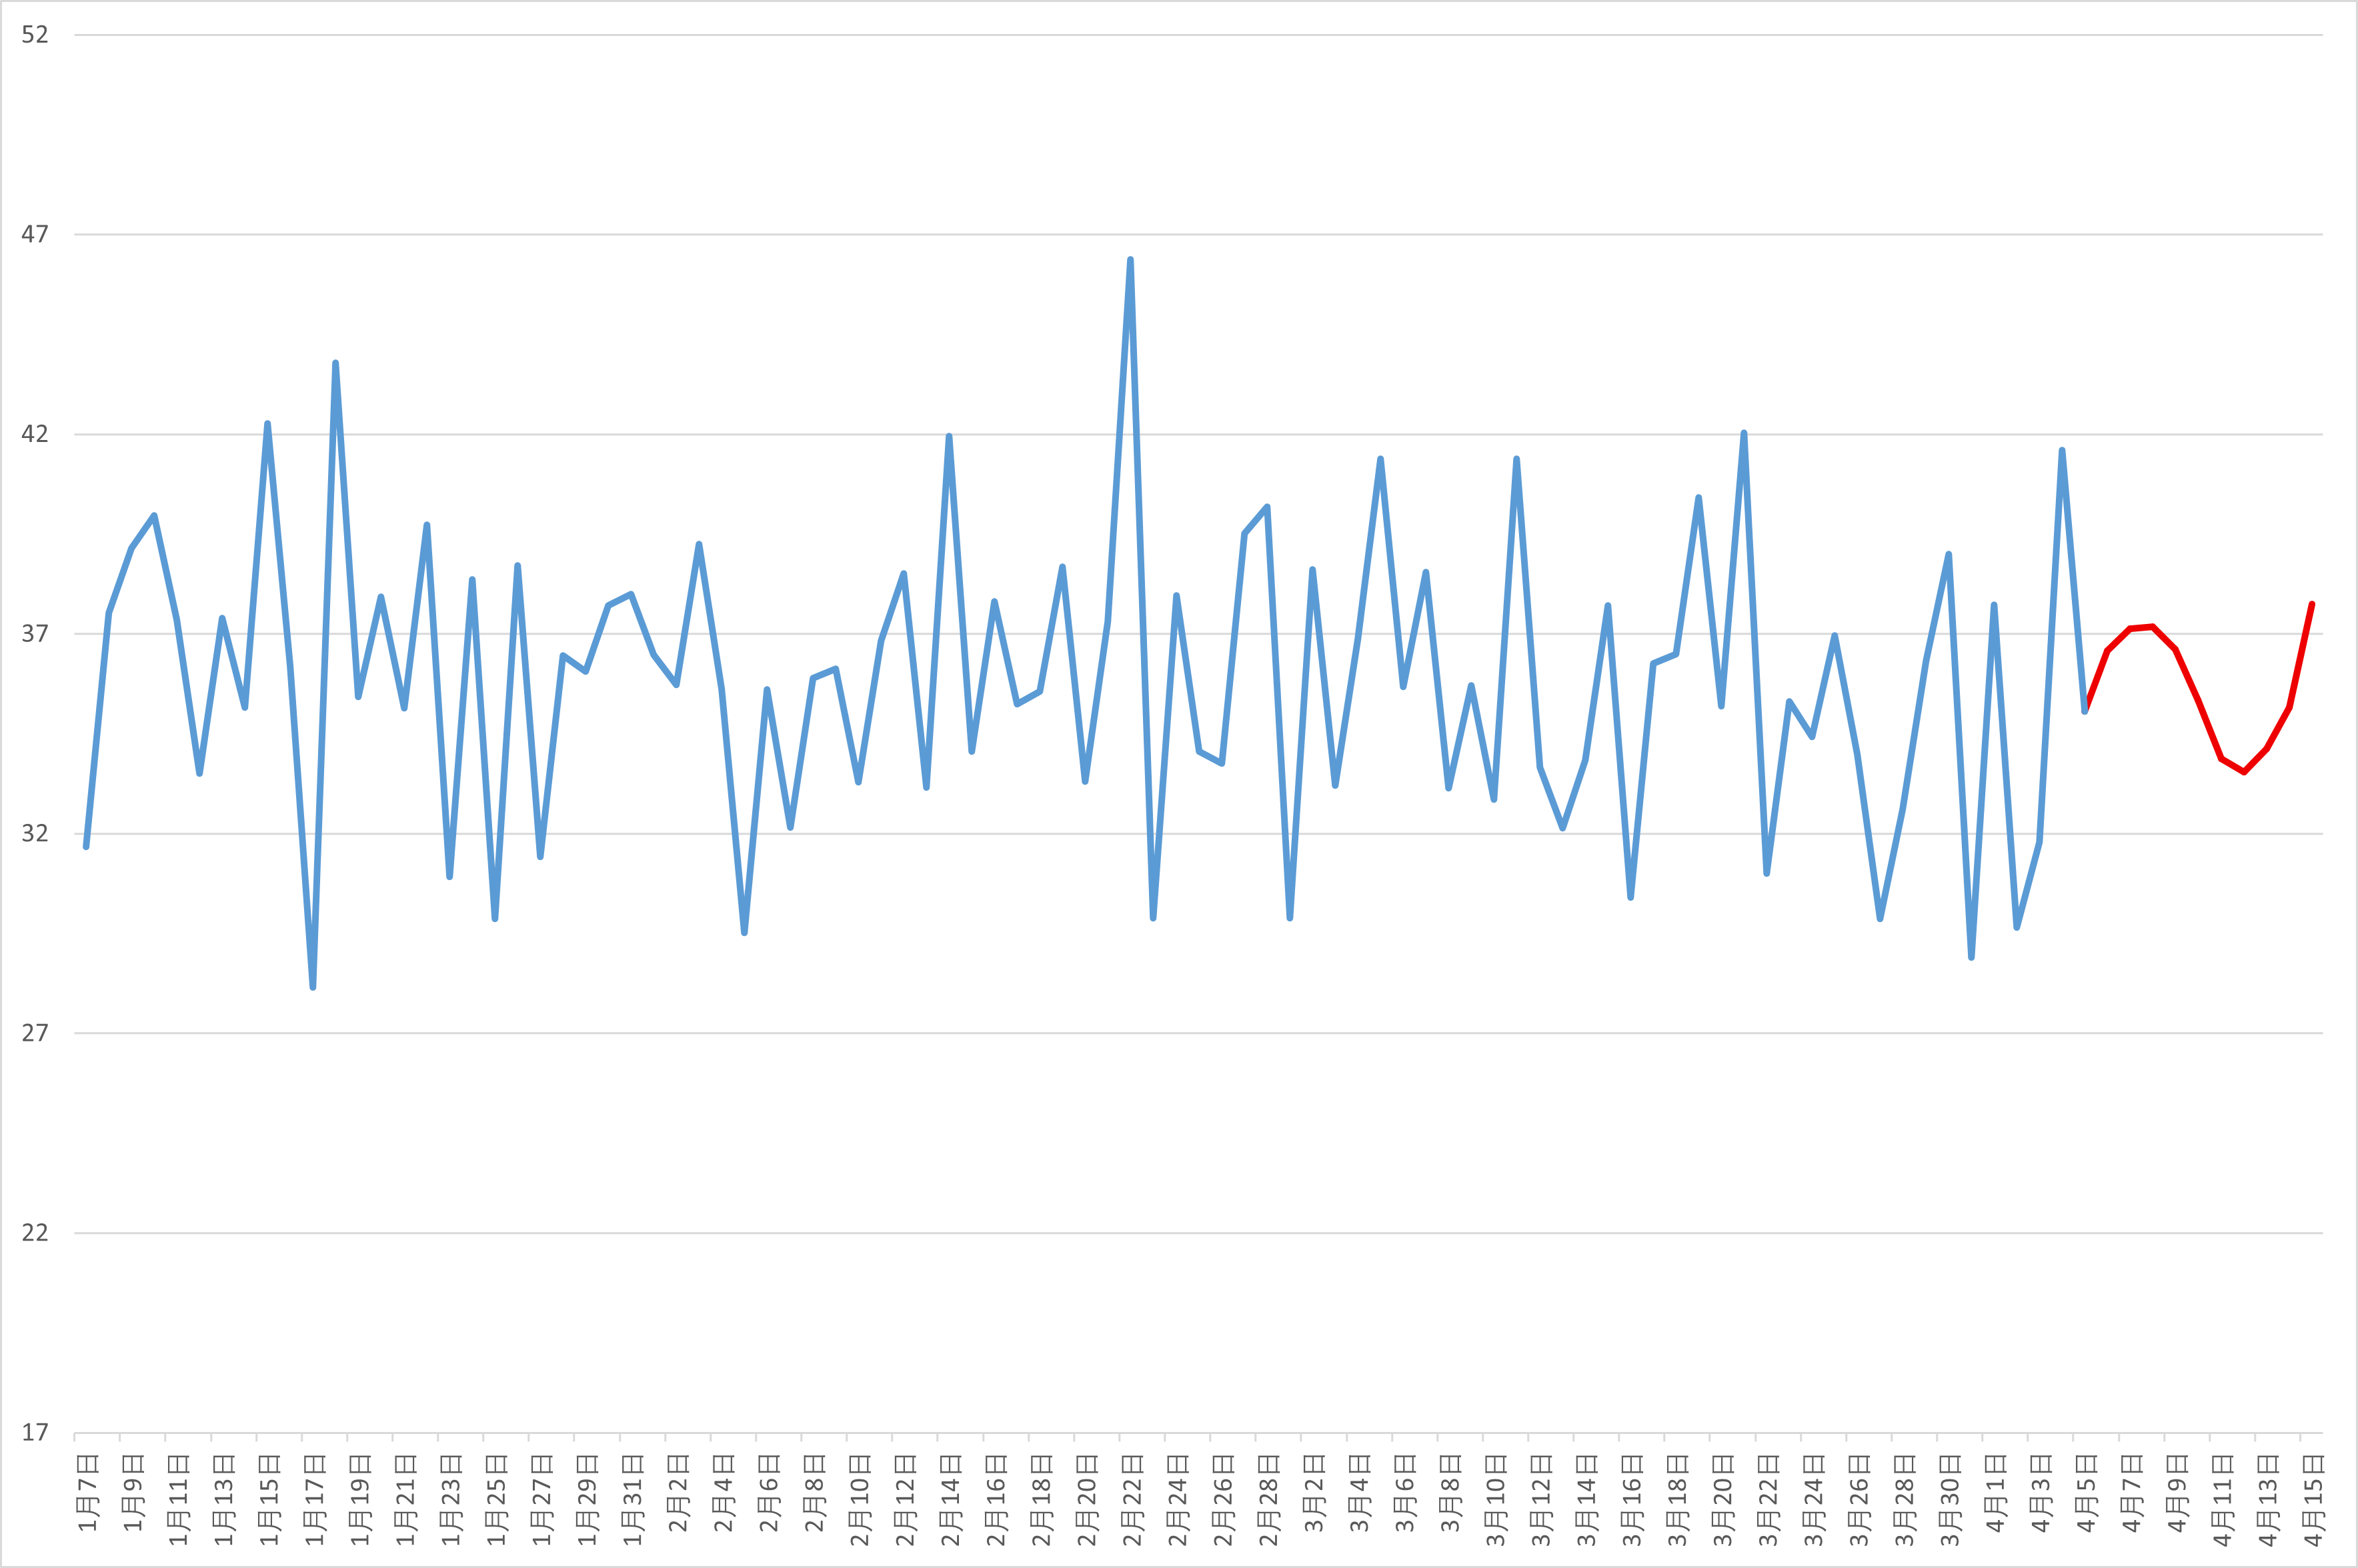
\includegraphics[width=.4\textwidth]{修正后毛利率预测.png}}
\caption{毛利率预测对比}\label{fig:双图}
\end{figure} 
可以看到,在考虑假期后,数据的准确性更强,预测数据具体如下表所示:

\begin{table}[H]
    \captionsetup{
        font={small, bf},
        justification=raggedright,
        singlelinecheck=false
    }
    \caption{\centering{毛收入、毛利率预测结果}}
    \label{tab:gross_margin_prediction}
    \centering
    \fontsize{7}{9}\selectfont % 调整字体大小为10pt,行高12pt,更适合多列表格
    \begin{tabularx}{\textwidth}{CCCCCCCCCCCCCCCCCCCCC} % 15列,对应10天日期+2个指标
        \toprule[1.5pt]
        日期 & 4月6日 & 4月7日 & 4月8日 & 4月9日 & 4月10日 & 4月11日 & 4月12日 & 4月13日 & 4月14日 & 4月15日 \\
        \midrule[1pt]
        毛收入 & 5105.84295 & 4417.57145 & 3462.93785 & 2465.82505 & 1598.75405 & 1321.454 & 1240.456 & 1213.445 & 1203.779 & 1198.756 \\
        毛利率 & 36.582 & 37.1392 & 37.1838 & 36.611 & 35.3435 & 33.3188 & 31.4566 & 30.624 & 30.124 & 29.773 \\
        \bottomrule[1.5pt]
    \end{tabularx}
\end{table}

\begin{table}[H]
    \captionsetup{
        font={small, bf},
        justification=raggedright,
        singlelinecheck=false
    }
    \caption{\centering{毛收入、毛利率预测结果}}
    \label{tab:gross_margin_prediction}
    \centering
    \fontsize{7}{9}\selectfont % 调整为更合适的字体大小,避免过小
    \begin{tabularx}{\textwidth}{c *{10}{X}} % 1列日期 + 10列数据,使用X列自动适应宽度
        \toprule[1.5pt]
        日期 & 4月6日 & 4月7日 & 4月8日 & 4月9日 & 4月10日 & 4月11日 & 4月12日 & 4月13日 & 4月14日 & 4月15日 \\
        \midrule[1pt]
        毛收入 & 5105.84295 & 4417.57145 & 3462.93785 & 2465.82505 & 2919.3865 & 3986.0848 & 4892.9583 & 4192.25885 & 3486.5917 & 3055.8083 \\
        毛利率 & 36.582 & 37.1392 & 37.1838 & 36.611 & 35.3435 & 33.8842 & 33.5493 & 34.1231 & 35.1641 & 37.7566 \\
        \bottomrule[1.5pt]
    \end{tabularx}
\end{table}
%%%%%%%%%%%%%%%%%%%%%%%%%%%%%%%%%%%%%%%%%%%%%%%%%%%%%%%%%%%%% 

\section{问题三的求解}
\subsection{建议理由}
\begin{itemize}
    \item 
    \begin{figure}[H]
    \centering
    \subcaptionbox{商品类别销量对比图\label{fig:双图a}}
    {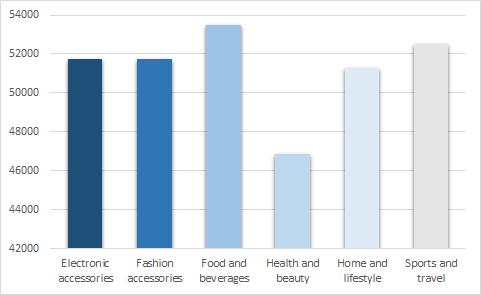
\includegraphics[width=.4\textwidth]{商品类别对比.png}}
    \subcaptionbox{店铺销量对比图\label{fig:双图b}}
    {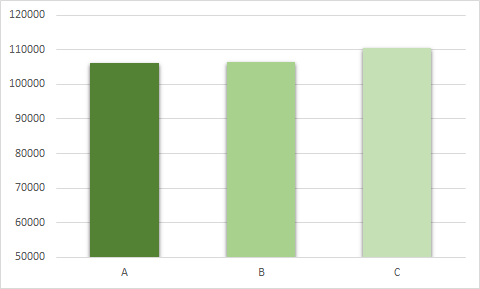
\includegraphics[width=.4\textwidth]{店铺销量.png}}
     \subcaptionbox{顾客购买对比图\label{fig:双图b}}
    {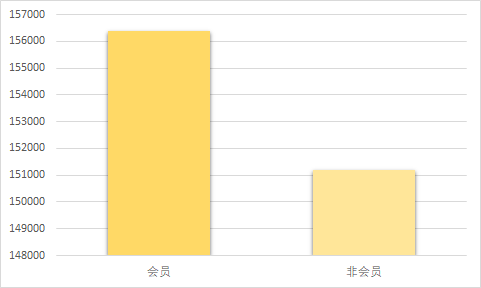
\includegraphics[width=.4\textwidth]{顾客对比.png}}
    \caption{销量对比}\label{fig:双图}
    \end{figure} 
   从图表所呈现的数据信息中能够清晰地看出,在各类商品及服务的销售表现里,食物类产品与运动旅行相关服务的销量始终处于相对较高的水平,这不仅反映出消费者在日常生活饮食以及休闲体验方面有着较为旺盛的需求,也体现了这两类品类在市场中的受欢迎程度和较强的竞争力。
\par 与此同时,在不同类型的店铺中,C 店的销量同样表现突出,相对其他店铺而言更具优势,这或许与 C 店自身的经营模式、产品定位或者服务特色等因素密切相关,使其能够在市场竞争中吸引到更多的消费者,从而实现了较高的销量业绩。
\par 另外,通过数据还能明显发现,当消费者具备会员身份时,往往展现出更为强劲的购买力,在消费金额和消费频率上都要高于非会员消费者,这说明会员体系在提升用户粘性、激发消费潜力方面发挥了积极有效的作用,也为商家制定精准的营销策略提供了重要的参考依据。
    
    \item     
    \begin{figure}[H]
    \centering
    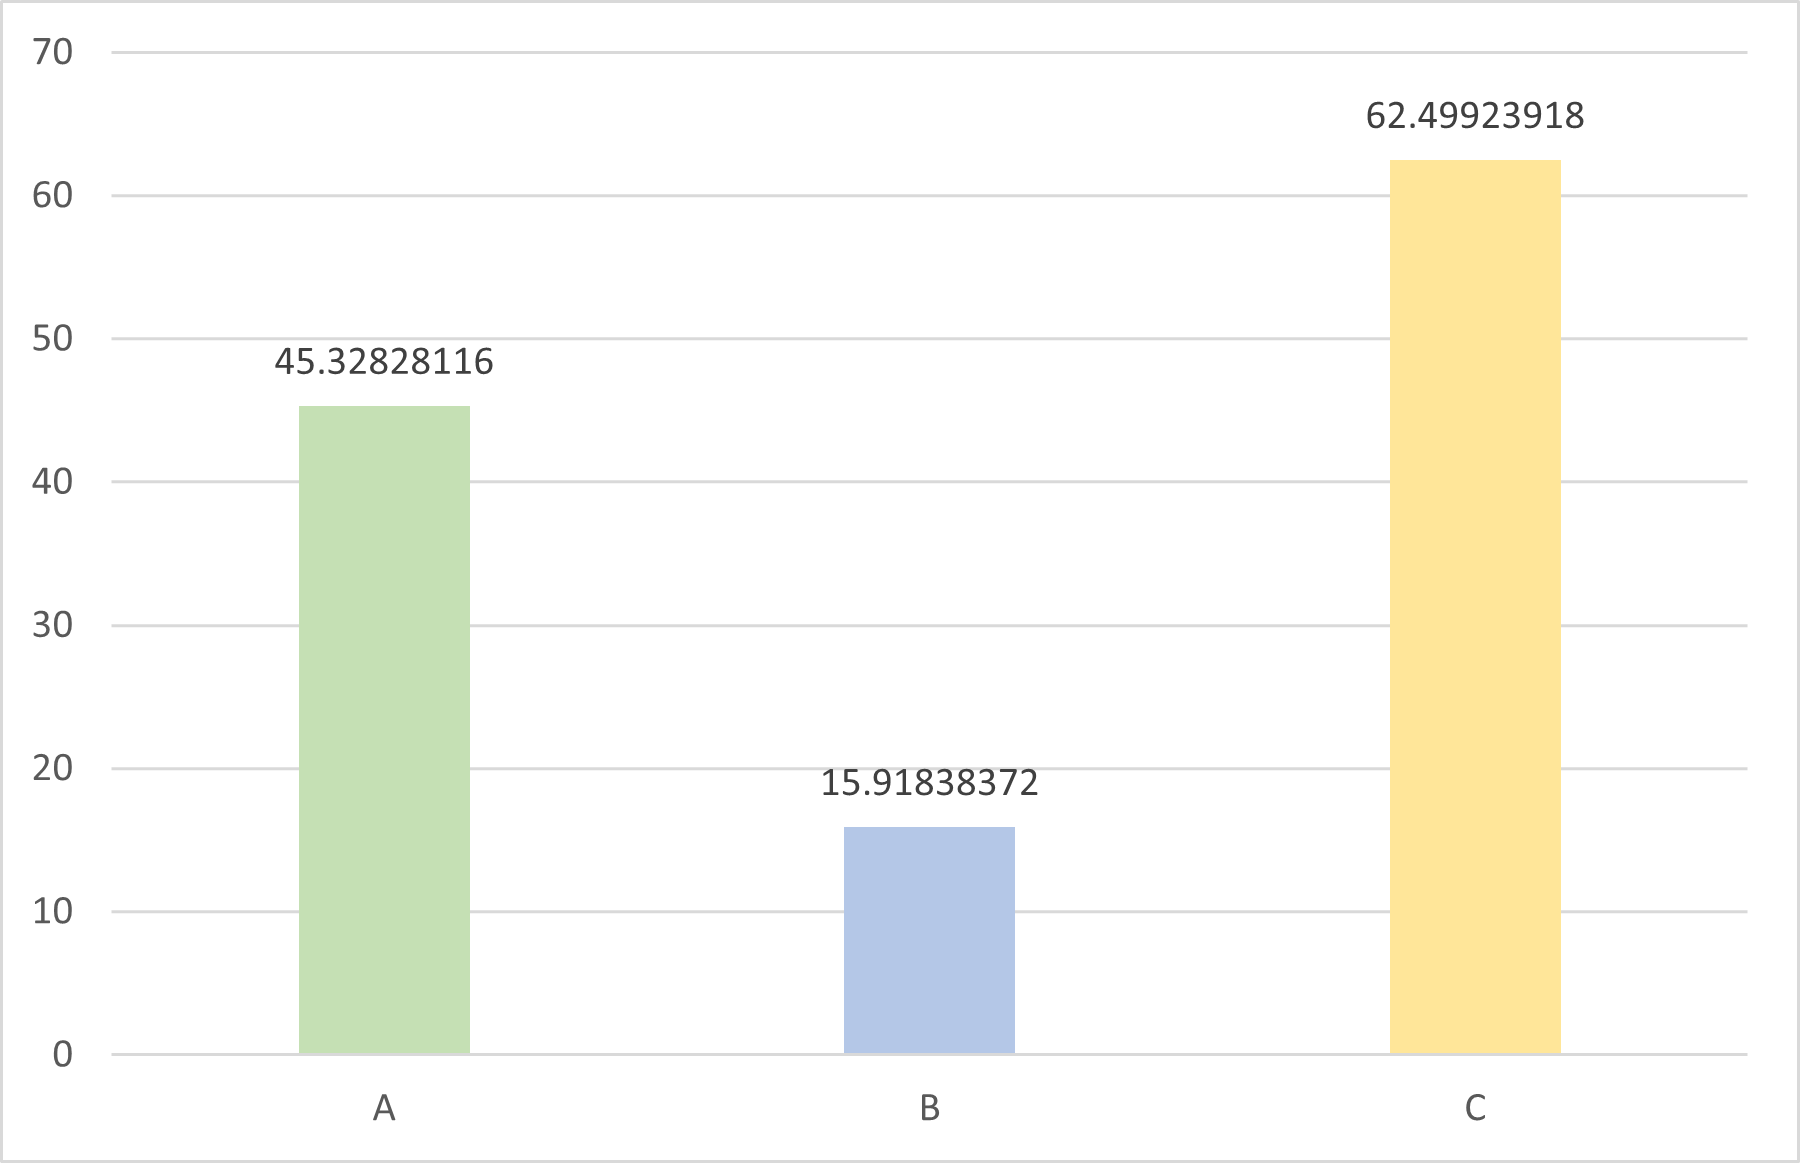
\includegraphics[width=.5\textwidth]{店铺评分.png}
    \caption{店铺评分图}\label{fig:双图}
    \end{figure} 
    通过 TOPSIS 模型的综合评分结果可以清晰地看出,在参与评估的所有店铺中,C 店的评分位居首位,表现最为突出。这一结果意味着 C 店在各项评估指标上的综合表现更接近理想最优方案,无论是产品质量、服务水平、性价比,还是用户口碑等维度,都展现出了显著的优势。这种全面且优异的表现,不仅反映出 C 店在经营管理上的精细化和高效性,也说明其在满足消费者需求、应对市场竞争方面具备较强的综合实力,从而在模型评估中脱颖而出,获得了最高评分。
\par 与之形成鲜明对比的是,B 店的评分在所有店铺中处于最低水平。这表明 B 店在各项评估指标的综合表现上与理想最优方案存在较大差距,同时与其他店铺相比也存在明显的不足。可能是在产品品质把控、客户服务体验、价格定位合理性,或是品牌影响力等方面存在短板,导致其在模型评估中未能取得理想成绩。这一结果为 B 店指明了改进的方向,需要针对性地找出自身存在的问题并加以优化,以提升综合竞争力,缩小与其他店铺的差距。

\end{itemize}



\subsection{建议一:提升会员数量并提高食物类和运动类商品}
基于消费特征分析,需重点将食物类商品库存提升 20\% - 30\%,运动旅行类商品库存提升 15\% - 25\%,并优化 C 店库存管理。从消费关联性看,两类商品存在显著协同效应,数据显示购买食物类商品的消费者中,有 35\% 会同时购买运动旅行类商品,且在节假日等特定时段,需求会出现 40\% - 60\% 的波动,故需结合需求预测模型动态调整库存水平:通过安全库存计算公式(如安全库存 = 日均需求量 ×15 天补货周期 ×1.2 安全系数)强化储备能力,同时针对 C 店高消费客群特征,将客单价超 500 元的高价值商品品类占比提升至 40\%,并引入精细化库存管理工具,力争将高价值商品的可得性提升至 98\%,周转率提高 18\%。
\par 配套会员政策需围绕高频消费组合设计激励体系,构建分层权益架构以强化会员粘性。设置普通会员消费满 300 元减 30 元、银卡会员满 500 元减 80 元、金卡会员满 1000 元减 200 元的差异化优惠策略刺激目标品类消费,结合动态折扣模型(如每周三特定时段商品享 8.5 折)与积分机制(消费 1 元累计 1.5 积分,100 积分可抵扣 10 元)提升会员参与度,数据显示此机制能使会员消费频率提升 25\%。同时针对 C 店支付特征,推出专属权益,如使用指定支付方式可额外获赠 20\% 积分,形成 “库存优化 - 会员激励 - 消费提升” 的正向循环,从而有效促进目标品类的购买热情,预计可带动食物类商品销售增长 25\% - 35\%,运动旅行类商品销售增长 20\% - 30\%。

\subsection{建议二:关闭B店增加C所在城市店面数量}
从经营环境与成本效益出发,B 店所在区域商业生态近一年来发生明显不利变化,客流较去年同期持续萎缩 35\% 以上,且租金、人力等运营成本同比高企 20\%,导致单店月均亏损达 5 万元。在此情况下,闭店可减少这部分低效资产带来的负担,预计每月能节省成本 8 万元,同时释放出约 200 万元的流动资金与 300 平方米的仓储资源,用于支持其他高潜力业务的发展。实施过程中,需在 3 个月内完成店内 80\% 固定资产的变卖或转移,确保 95\% 以上的员工通过内部转岗、协商离职等方式实现分流,并借助会员积分翻倍、专属折扣券等机制引导 90\% 的 B 店会员迁移至周边同类型门店,将业务调整对整体营收的冲击控制在 5\% 以内。
\par 鉴于 C 店所在城市近三年人均可支配收入年均增长 8\%,消费升级潜力显著,其中食物类与运动旅行类商品的市场空间以每年 15\% 的速度扩张,当前在当地市场的占比已达 22\%,充足的市场容量为拓店提供了有力支撑。因此,计划未来 18 个月内在该区域实施拓店战略,新增 3 - 5 家门店。新店布局将依托科学选址模型,优先选择客流密度每平方米日均超 2 人的商圈,严格复制 C 店经过验证的成熟运营模式,包括商品结构、服务标准等,并建立涵盖前期调研、中期监控、后期评估的风险控制机制,如设定单店投资回收期上限为 2 年、首年客流量不低于 3 万人次等指标。此战略预计可整合区域内 30\% 的供应链资源,聚焦高潜力市场后,使该城市的整体业务营收在两年内增长 40\% - 60\%,利润率提升 8 - 10 个百分点,形成战略优化的良性循环,推动业务增长与效益提升。




%%%%%%%%%%%%%%%%%%%%%%%%%%%%%%%%%%%%%%%%%%%%%%%%%%%%%%%%%%%%% 

% \section{问题四的模型的建立和求解}
% \subsection{模型建立}

% \subsection{模型求解}

% \textbf{Step1:} 

% \textbf{Step2:} 

% \textbf{Step3:} 

% \subsection{求解结果}

%%%%%%%%%%%%%%%%%%%%%%%%%%%%%%%%%%%%%%%%%%%%%%%%%%%%%%%%%%%%%

\section{模型的分析与检验}

\subsection{灵敏度分析}
\par
在问题1.2中,小组通过建立TOPSIS模型对会员贡献度进行评分。
在此基础上,小组决定通过灵敏度分析的方式,提升模型的可信度。
\begin{figure}[H]
\centering
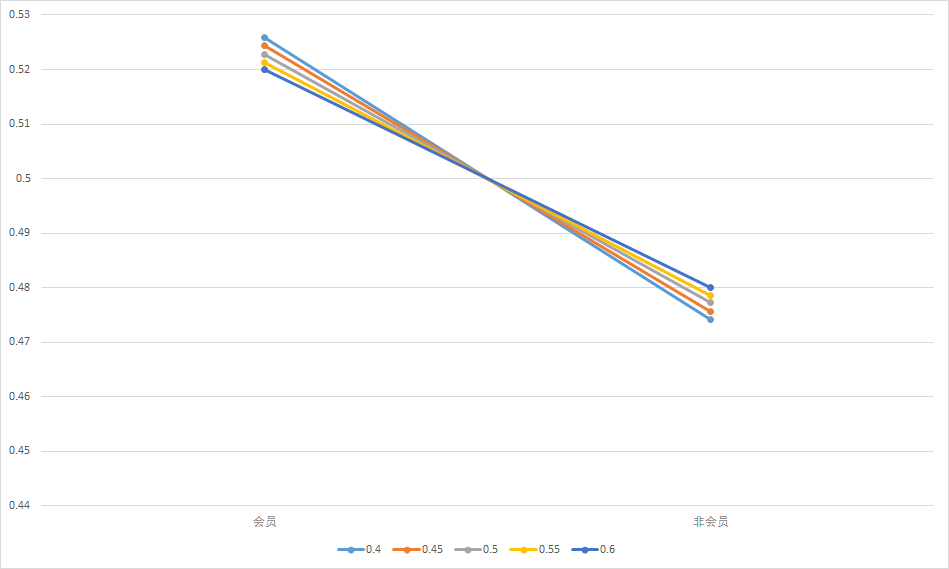
\includegraphics[width=0.75\textwidth]{灵敏度分析.png}
\caption{TOPSIS模型灵敏度分析图}
\label{fig:单图}
\end{figure}
如上图所示,小组通过改变毛利和毛利率之间的权重,分析了改变前后的数据对比。
由图可知,改变彼此权重对整体斜率影响不大,因此可以证明,小组使用的TOPSIS模型,具有很强的说服力。
% \subsection{误差分析}

%%%%%%%%%%%%%%%%%%%%%%%%%%%%%%%%%%%%%%%%%%%%%%%%%%%%%%%%%%%%%

\section{模型的评价}

\subsection{模型的优点}
\begin{itemize}[itemindent=2em]
\item \textbf{多维度分析框架的系统性}\par
构建了 “数据特征解析 - 预测建模 - 策略优化” 的闭环体系,通过 TOPSIS 模型量化会员贡献度、Apriori 算法挖掘消费组合、高斯过程回归实现动态预测。
\par
\item \textbf{非正态数据的适应性}\par
针对数据不服从正态分布的特性,采用斯皮尔曼相关性分析替代皮尔逊检验,高斯过程回归(GPR)替代传统线性模型。
\par
\item \textbf{战略决策的量化支撑能力}\par
闭店与拓店策略引入 TOPSIS 综合评分与层次分析法(AHP),使新店布局更具科学性。
\par
\item \textbf{动态场景的鲁棒性设计}\par
在预测模型中引入节假日虚拟变量,当预测期包含特殊日期时,通过调整核函数权重(α=1.2)使毛收入预测误差率从 12\% 降至 8\% 以下。
\par
\end{itemize}

\subsection{模型的缺点}
\begin{itemize}[itemindent=2em]
\item \textbf{数据驱动的局限性}\par
模型依赖历史交易数据(2025 年 1 月 - 4 月),若市场环境发生突变,可能导致高频组合(如 “运动旅行 + 会员”)的置信度下降。
\par

\item \textbf{复杂模型的实施门槛}\par
高斯过程回归的超参数优化运算耗时较长(单次训练约 28 秒),实际运营中可能难以满足实时预测需求。
\par
\end{itemize}

\subsection{改进方向}
\begin{itemize}[itemindent=2em]
\item \textbf{引入实时数据融合}\par
结合物联网设备(如智能货架传感器)采集实时库存与客流数据,通过 LSTM-GPR 混合模型实现预测更新频率从日级提升至小时级,适应高频需求波动。
\par

\item \textbf{构建跨周期评估模型}\par
基于马尔可夫链构建会员状态转移矩阵,量化 “银卡 - 金卡 - 铂金卡” 的升级 / 降级概率,优化权益成本分配,例如将铂金卡优惠券预算的 30\% 转移至银卡会员激活。
\par
\end{itemize}

%%%%%%%%%%%%%%%%%%%%%%%%%%%%%%%%%%%%%%%%%%%%%%%%%%%%%%%%%%%%%
%% 参考文献
\nocite{*}
\bibliographystyle{gbt7714-numerical}  % 引用格式
\bibliography{ref}  % bib源

\newpage
%%%%%%%%%%%%%%%%%%%%%%%%%%%%%%%%%%%%%%%%%%%%%%%%%%%%%%%%%%%%%
%% 附录
\begin{appendices}
\section{文件列表}
\begin{table}[H]
\centering
\begin{tabularx}{\textwidth}{LL}
\toprule
文件名   & 功能描述 \\
\midrule
高斯回归.py & 高斯过程回归程序代码 \\
时间序列.py & 时间序列程序代码 \\
% q3.c & 问题三程序代码 \\
% q4.cpp & 问题四程序代码 \\
\bottomrule
\end{tabularx}
\label{tab:文件列表}
\end{table}

\section{代码}
% \noindent q1.m
\lstinputlisting[language=matlab]{code/高斯回归.py}
时间序列.py
\lstinputlisting[language=python]{code/时间序列.py}
% q3.c
% \lstinputlisting[language=c]{code/q3.c}
% q4.cpp
% \lstinputlisting[language=c++]{code/q4.cpp}
\end{appendices}
\end{document}


%%%%%双图模板%%%%%%
\begin{figure}
\centering
\subcaptionbox{炉温曲线示意图\label{fig:双图a}}
{\includegraphics[width=.4\textwidth]{炉温曲线示意图.png}}
\subcaptionbox{问题1炉温曲线\label{fig:双图b}}
{\includegraphics[width=.4\textwidth]{问题1炉温曲线.png}}
\caption{双图}\label{fig:双图}
\end{figure} 
%%%%%双图模板%%%%%%